\documentclass[11pt]{article}
\usepackage[utf8]{inputenc}
\usepackage[spanish, es-tabla]{babel}
\usepackage{amsmath}
\usepackage{amsfonts}
\usepackage{amssymb}
\usepackage{amsthm}
\usepackage{makeidx}
\usepackage[pdftex]{graphicx}
\usepackage[a4paper, margin=2.75cm, bottom=3.25cm, top=2.25cm]{geometry}
\usepackage[hidelinks,breaklinks]{hyperref}
\usepackage[usenames, dvipsnames]{color}
\usepackage{float}
\usepackage{afterpage}
\usepackage{array}
\usepackage{multirow}
\usepackage{forloop}
\usepackage{longtable}
\usepackage{ulem} % Arregla los problemas asociados a underline
\setlength{\parindent}{0pt}
\usepackage{footnote}
\usepackage{pdfpages}
\usepackage{enumerate}
\newcommand\blankpage{%
    \null
    \thispagestyle{empty}%
    \addtocounter{page}{-1}%
    \newpage}
% Necesitamos resetear las secciones en cada tema
\makeatletter 
\@addtoreset{section}{part}
\makeatother  

\begin{document}
\renewcommand\partname{Tema} %Cambio de "parte" por "tema"
\includepdf{Resources/PORTADA.pdf}
\blankpage
% Portada de los apuntes de ENSO
% RESUMEN DE ENSO
% AHORA CON MÁS RABO! (mensaje superior derecha)
% INCLUYE PREGUNTAS DE EXAMEN! (en vertical)
% EDICIÓN ESPECIAL TABOADA 2016-2017(mensaje inferior izquierda)

\tableofcontents
\newpage
\part{El Software}
\paragraph{Software}
% Instrucciones de ordenador que cuando se ejecutan proporcionan la función y el comportamiento deseado, estructuras de datos que facilitan a los programas manipular adecuadamente la información, y documentos que describen la operación y el uso de los programas.
% \\\\
\textit{Pressman} define el software como el conjunto de \textbf{código, estructuras de datos y documentación} asociados a un sistema, y particularmente a un sistema computacional.

\section{Características}
El software se diferencia de los productos de otras ingenierías por lo siguiente:
\begin{enumerate}

    \item \textbf{Curva de fallos con respecto al tiempo diferente}:
    El software no se estropea con el tiempo, sin embargo es común aplicar ciertos cambios al mismo durante su ciclo de vida, lo cual va degradando su calidad de manera irreversible.
    \begin{figure}[h]
        \centering
        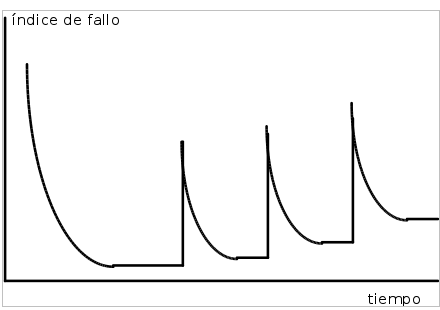
\includegraphics[width=0.4\textwidth]{Resources/fallosSoftwareReales.png}
        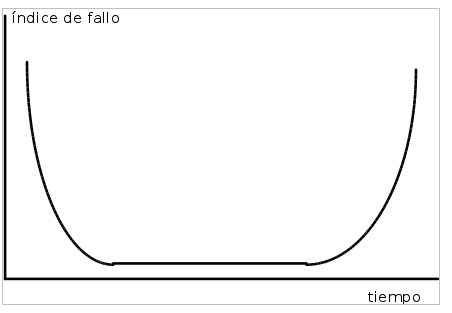
\includegraphics[width=0.4\textwidth]{Resources/fallosHardware.png}
        \caption{Curva de fallos del Software(Izquierda) y del Hardware(Derecha). Obsérvese como en el caso del software el índice de fallos se va acumulando.}
    \end{figure}
    \item \textbf{Baja reutilización de las partes}:
    Por lo general el software se construye a medida como un conjunto, provocando que la reutilización sea baja. Existe una tendencia al alza en la reutilización gracias a:
    \begin{itemize}
        \item La elaboración de librerías y frameworks.
        \item Aplicación de técnicas de programación modular y orientada a objetos de manera estructurada. 
        \item Aplicación de patrones de diseño, que supone en sí misma la reutilización de la estructura ahorrando tiempo en diseño y formación.
    \end{itemize}
\end{enumerate}

\section{Atributos deseables en el software}
\begin{itemize}
    \item \textbf{Mantenibilidad}: Facilidad para realizar cambios.
    \item \textbf{Confiabilidad}: Capacidad para seguir funcionando de manera segura y correcta. 
    \item \textbf{Eficiencia}: Utilización de la mínima cantidad necesaria de recursos.
    \item \textbf{Usabilidad}: Facilidad con la que las personas utilizan el software.
\end{itemize}

\subsection{Aplicaciones del software}
Es difícil clasificarlas y carece de mucho valor hacerlo, \textit{Pressman} lo hace de la siguiente forma, si pregunta características no es difícil deducirlas:
\begin{itemize}
    \item \textbf{Software de sistemas}: Sistemas operativos.
    \item \textbf{Software de aplicación}: Programas independientes que resuelven una necesidad específica.
    \item \textbf{Software científico y de ingeniería}: Simulaciones.
    \item \textbf{Software empotrado}: Corre él solo en un chip.
    \item \textbf{Software de línea de productos}: \textit{Middleware}.
    \item \textbf{Aplicaciones web}.
    \item \textbf{Inteligencia artificial}: \textit{Redes neuronales} (máquinas de estados \textbf{NO}).
\end{itemize}
El objetivo de todo software es desempeñar una determinada función cumpliendo una serie de requisitos.

\section{Software heredado}
Se trata de software \textbf{desarrollado hace décadas} %CORBA 
que además \textbf{ha ido sufriendo cambios} a lo largo del tiempo. Estos dos factores hacen que sea muy difícil de tratar, \uline{y usualmente es crítico para los negocios} (COBOL). \textit{Pressman} aconseja tocarlo lo mínimo posible. 

\section{Principales problemas asociados a la producción del software}
Muchos expertos argumentan que la crisis del software nunca se ha solucionado, y es que esta ingeniería arrastra desde hace tiempo los siguientes \textbf{problemas crónicos}.
\begin{enumerate}
    \item \textbf{Imprecisión en la estimación de costes temporales y monetarios}: Entre las causas podemos citar la falta de recogida de datos de proyectos anteriores y la tradicional falta de experiencia de los gestores (gente que no tiene ni idea de software gestionando proyectos o viceversa).
    \item \textbf{Baja productividad}: El poco énfasis en la recogida de requisitos comúnmente desemboca en tiempo de desarrollo malgastado. Ya bien sea implementando funcionalidad innecesaria o bien por implementarla en un estado de desarrollo avanzado, lo cual es mucho más costoso.
    \item \textbf{Mala calidad}: La falta de realización de pruebas, debida en gran medida a los fallos anteriores, propicia la entrega de software con muchos errores.
    \item \textbf{Insatisfacción del cliente}: Debida a los problemas anteriores no es una tarea agradable contratar software.
\end{enumerate}
\newpage
\part{El proceso}

\section{Conceptos}
\paragraph{Ingeniería del Software} Aplicación de un enfoque sistemático, disciplinado y cuantificable hacia el desarrollo, operación y mantenimiento del software; es decir, la aplicación de la ingeniería al software. (IEEE). %La que más le gusta al rabo es la que hay que saberse. No es dificil hecharle mas royo

% Esto se define en el siguiente capítulo mejor, ¿lo eliminamos y ponemos referencia al Tema 3? -> Fuera nada de redundancia XD


%Adaptadas y añadadidas las definiciones del rabo de las traspas, de abajo a arriba porque es como tiene el rabo
\paragraph{Tarea} Cualquier acción que transforma una entrada en salidas, el objetivo debe de ser pequeño y bien definido. \textit{Ej: Ejecución del caso de prueba}.


\paragraph{Actividad} Conjunto de tareas que producen un producto importante del trabajo. \textit{Ejemplo: desarrollo de un plan de pruebas.}

\paragraph{Proceso} Conjunto de actividades, y tareas que se ejecutan para llevar a cabo algún producto de trabajo. Este conjunto es \textbf{adaptable} a las necesidades del que lo utiliza. \textit{Ejemplo: Validación}.


\paragraph{Modelo de los procesos} Descripción de los procesos involucrados en el desarrollo del software sin especificar cuando se desarrolla: \textit{Ejemplos: IEEE 1074, ISO 12207-1 e ISO/IEC TR 15504-2}.


\paragraph{Métodos y procedimientos} Determinan el modo en el que se \textit{ejecutan las tareas}, determinando qué técnicas se utilizan en cada fase y cómo. \textit{Ejemplo: IEEE 1008}.

\paragraph{Técnica} Cualquier recurso utilizado para llevar a cabo una tarea. Normalmente hablamos de gráficos con apoyos textuales.\textit{ Ej: Cobertura de caminos}.

\paragraph{Herramienta} Cualquier software que nos ayude en cualquier etapa del desarrollo. \textit{Ejemplo: JUnit}.

% TODO metodologia y ciclos de vida faltan o se han suprimido por algun motivo?


\section{Procesos para la construcción del software}


% Pongo las del pressman MODERNO (6-7) Edición porque están mejor hechos

% La construcción del software incluye una serie de actividades que se empiezan a estandarizar. \textit{Pressman} divide la construcción de software en 
% \textbf{3 fases}, en cada una de las cuales se debe responder a alguna de las siguientes preguntas: ¿cuál es el problema a resolver?, ¿cuáles son las características de la entidad que se utiliza para resolver este problema?, ¿cómo se realizará la entidad?, ¿qué enfoque se va a utilizar para no contemplar los errores que cometieron en el diseño y la construcción de la entidad?, ¿cómo se sostendrá la entidad cuando los usuarios soliciten correcciones, adaptaciones y mejoras de la entidad?

% \begin{enumerate}
%     \item \textbf{Fase de definición}: Intenta identificar la información a procesar, la función y rendimiento esperados, las restricciones de diseño, las interfaces a utilizarse, los sistemas operativos y de hardware a utilizar, y los criterios de validación. Se identifican 3 actividades:
%     \begin{itemize}
%         \item \textbf{Análisis del sistema}: Define el papel de cada elemento relacionado con el sistema informático a desarrollar.
%         \item \textbf{Análisis de requisitos del software}: Proporciona el ámbito del software y su relación con el resto de componentes del sistema.
%         \item \textbf{Planificación}: Organización de las tareas que se llevarán a cabo en el proyecto. Existen dos formas de analizar los requisitos del software:
%         \begin{itemize}
%             \item Análisis formal del ámbito de la información para establecer modelos del flujo y la estructura de la información.
%             \item Construcción de un prototipo evaluado por el cliente para intentar consolidar los requisitos
%         \end{itemize}
        
%         Es una tarea que debe ser llevada a cabo conjuntamente por el desarrollador de software y el cliente. \uline{Esta etapa produce el documento de especificación de requisitos del software.}
%     \end{itemize}
%     \item \textbf{Desarrollo}: Intenta definir cómo han de diseñarse las estructuras de datos, cómo ha de implementarse la función dentro de una arquitectura software, cómo han de implementarse los detalles procedimentales, cómo han de caracterizarse las interfaces, cómo ha de traducirse el diseño en un lenguaje de programación y cómo ha de realizarse la prueba. Se definen 3 actividades: 
%     \begin{itemize}
%         \item \textbf{Diseño del software}.
%         \item \textbf{Codificación}.
%         \item \textbf{Pruebas}.
%     \end{itemize}
%     \item \textbf{Mantenimiento}: Se centra en el cambio asociado a la corrección de errores, a las adaptaciones requeridas a medida que evoluciona el entorno del software, y a los cambios debidos a las mejoras producidas por los requisitos cambiantes del cliente. Se definen 4 actividades:
%     \begin{itemize}
%         \item \textbf{Corrección}
%         \item \textbf{Adaptación}
%         \item \textbf{Mejora}
%         \item \textbf{Prevención}
%     \end{itemize}
% \end{enumerate}


\textit{Pressman} define dos conjuntos de tareas en lo que él denomina el proceso del software:

\paragraph{Actividades estructurales} Son aplicables en todo tipo de software sin importar su tamaño.\\\\
\textbf{Nota:} \textit{Estas actividades se aplican de forma iterativa según la última versión del Pressman. Por ejemplo un proceso de mantenimiento como puede ser la corrección de un error grande encajaría como una iteración de este modelo y no como una actividad concreta.}

\begin{itemize}
    \item \textbf{Comunicación.} Se busca entender los objetivos de los participantes, y reunir los \textbf{requisitos, características y funciones} del software.
    
    \item \textbf{Planificación.} Define el trabajo de ingeniería de un software al describir las tareas que se van a realizar, los riesgos, los productos de trabajo, y una programación de actividades.
    
    
    \item \textbf{Modelado.} Creación de un ``bosquejo'' con el objetivo de entender mejor el problema y cómo resolverlo.
    
    \item \textbf{Construcción.} Incluye la codificación y las pruebas para descubrir sus errores.
    
    \item \textbf{Despliegue.} Entrega y puesta a punto del software para el cliente, que lo evalúa y provee un \textit{feedback}.
\end{itemize}


\paragraph{Actividades sombrilla} Son aplicadas a lo largo de todo el proceso del software de manera complementaria.
\begin{itemize}
 \item Seguimiento y control del proyecto.
 \item Administración de riesgos
 \item Aseguramiento de la calidad.
 \item Revisiones técnicas.
 \item Gestión de la configuración. % léase con voz de rabenso
 \item Administración de la reutilización.
 \item Preparación y producción del producto de trabajo.

\end{itemize}



\subsection{Norma IEEE 1074}
Proporciona el conjunto de actividades que constituyen los procesos que son necesarios para el correcto desarrollo y mantenimiento del software. Los procesos se dividen en 4 secciones lógicas:

\begin{enumerate}
    \item \textbf{Proceso de Modelo del Ciclo de Vida Software}.  Actividades para seleccionar el modelo de ciclo que \textbf{mejor se adapte} al proyecto.
    \item \textbf{Procesos de gestión del proyecto}.
    \begin{itemize}
        \item \textbf{Proceso de iniciación del proyecto}: Se crea el ciclo de vida y se definen los planes y métricas (conjunto de medidas utilizadas) para la gestión del proyecto.
        \item \textbf{Proceso de supervisión y control del proyecto}: Proceso iterativo de seguimiento, informes y gestión de costes, calendarios, problemas y rendimiento de un proyecto a lo largo del ciclo de vida. El progreso se revisa y mide en los hitos establecidos.
        \item \textbf{Proceso de gestión de la calidad software}: aseguramiento de calidad, mejora de la misma y satisfacción del cliente.
    \end{itemize}
    \uline{Estas dos últimas actividades se llevan a cabo durante toda la vida del proyecto.}
    \item \textbf{Procesos Orientados al Desarrollo}. Comprenden los procesos que se realizan antes, durante y después del desarrollo software.
    \begin{itemize}
        \item Pre--desarrollo:
        \begin{itemize}
            \item Análisis de la necesidad del sistema.
            \item Asignación de requisitos \textbf{al desarrollo} software y hardware.
        \end{itemize}
        \item Desarrollo:
        \begin{itemize}
            \item Análisis de requisitos.
            \item Diseño de arquitectura, BBDD, interfaces\ldots
            \item Codificación, documentación operativa e integración.
        \end{itemize}
        \item Post--desarrollo:
        \begin{itemize}
            \item Instalación.
            \item Soporte.
            \item Mantenimiento.
            \item Retirada.
        \end{itemize}
    \end{itemize}
    \item \textbf{Procesos Integrales}: Necesarios para asegurar terminación y \textbf{calidad de los procesos}.
    \begin{itemize}
        \item Verificación y Validación.
        \item Gestión de Configuración Software.
        \item Desarrollo de documentación.
        \item Formación.
    \end{itemize}
\end{enumerate}

\subsection{Norma ISO 12207--1}
 Define una serie de actividades que se realizan en la construcción del software. No fomenta ningún modelo concreto de ciclo de vida, gestión del software o método de ingeniería, ni prescribe cómo realizar las actividades o cómo organizarlas.

\subsubsection{Procesos principales}
Los procesos principales resultan útiles a las personas que inician o realizan el desarrollo, la explotación o el mantenimiento del software durante su ciclo de vida. Los procesos principales son:
\begin{enumerate}
    \item \textbf{Proceso de adquisición}: Contiene las actividades y tareas realizadas por el cliente. \textit{Ej: Solicitud de ofertas}.
    \item \textbf{Proceso de suministro}: Contiene las actividades y tareas que realiza el suministrador. Incluye la preparación de la oferta y la identificación de los recursos y procedimientos para garantizar el éxito del proyecto.
    \item\textbf{Proceso de desarrollo}: Contiene las actividades de análisis de requisitos, diseño, codificación, integración, pruebas e instalación y aceptación. 
    \item \textbf{Proceso de explotación}: Contiene la explotación del software y el soporte operativo a los usuarios. Son tareas aplicadas al sistema completo.
    \item \textbf{Proceso de mantenimiento}: Modificación o documentación del software provocadas por errores, mejoras adaptaciones, migraciones o retiradas del sistema.
\end{enumerate}

\subsubsection{Procesos de soporte}
Sirven de apoyo al resto y se aplican en cualquier punto del ciclo de vida.
\begin{enumerate}
    \item \textbf{Proceso de documentación}: Registra la información producida por un proceso o actividad del ciclo de vida.
    \item \textbf{Proceso de gestión de la configuración}.
    \item \textbf{Proceso de verificación}: Determina si los requisitos de un sistema o del software están completos y son correctos, y si los \textbf{productos software de cada fase} del ciclo de vida cumplen los requisitos o condiciones impuestos en fases previas.
    \item \textbf{Proceso de validación}: Sirve para determinar si el \textbf{sistema o software final} cumple con los requisitos previstos para su uso.
    \item \textbf{Proceso de revisión conjunta}: Evaluación del estado del software y sus productos en su conjunto.
    \item \textbf{Proceso de auditoría}: Permite determinar, mediante hitos predeterminados, si se han cumplido los requisitos, los planes y el contrato.
    \item \textbf{Proceso de resolución de problemas}: Analiza y elimina los problemas descubiertos durante el desarrollo, la explotación, el mantenimiento u otro proceso.
    \item \textbf{Proceso de aseguramiento de la calidad}: Aporta la confianza de que los productos y procesos cumplen los requisitos y se ajustan a lo previsto utilizando los resultados de los procesos anteriores a partir de validación.
\end{enumerate}

\subsubsection{Procesos de la organización}
Ayudan a establecer, implementar y mejorar la organización, consiguiendo que sea más efectiva. Se llevan a cabo fuera del ámbito de proyectos y contratos específicos.

\begin{enumerate}
    \item \textbf{Proceso de gestión}: Planificación, seguimiento y control, evaluación \ldots
    \item \textbf{Proceso de infraestructura}: Dota a los procesos de la infraestructura necesaria, incluyendo hardware, software, normas, herramientas\ldots
    \item \textbf{Proceso de mejora}: Referente a los procesos del ciclo de vida.
    \item \textbf{Proceso de formación}: Mantener al personal formado, incluyendo materiales y planes de formación.
\end{enumerate}

\subsection{Norma ISO/IEC TR 15504--2}
Se puede considerar una ampliación a la norma ISO 12207 – 1 ya que \uline{amplía o añade procesos}. Los procesos que se añaden son los siguientes:


% Quizás dividirlos en listas a los categoría de procesos existentes a la que se añaden
% el rabenso solo pone esto en la traspa como una lista que ni se vé que a tomar por culo XD

\begin{itemize}
    \item Procesos Principales: \textbf{Obtención de requisitos}
    \item Procesos de Organización: Gestión de recursos humanos, alineamiento de la organización (misión, visión y valores), medida y reutilización. \textbf{El proceso de gestión se divide} en:
    \begin{itemize}
        \item Gestión \textbf{general}.
        \item Gestión del \textbf{proyecto}.
        \item Gestión de \textbf{calidad}.
        \item Gestión de \textbf{riesgos}.
    \end{itemize}
\end{itemize}

% El rabenso añadió:
\subsubsection{Estructura}
En este estándar la descripción de procesos tiene la siguiente estructura:
\begin{enumerate} % Te lo traduzco porque así se piensa menos
    \item Identificador. %Identifier
    \item Título.%Title
    \item Propósito.%Pruporse
    \item Outcomes: deben ser resultados observables.
    \item Actividades y tareas: lista de actividades y las tareas que componen dichas actividades.
\end{enumerate}
Además de definir procesos, también expresa la capacidad que una empresa ha logrado en el desarrollo de dicho proceso.\\



\section{Evaluación del proceso software}
Como respuesta a los problemas comentados en la \textit{la crisis del software} surgen una serie de métodos de evaluación y mejora de los procesos de la ingeniería del software.
\\\\
Objetivos:
\begin{itemize}
    \item \uline{De cara al contratante} de la empresa de software proporcionar una medida de \textbf{cuan confiable} es que la empresa ofrezca sus servicios de creación y mantenimiento de software en tiempo y forma.
    \item \uline{De cara a la desarrolladora} pretenden guiarla en la \textbf{mejora continua de sus procesos} de ingeniería.
\end{itemize}

\begin{figure}[H]
  \centering
  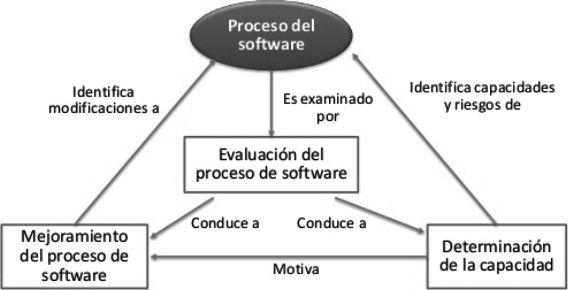
\includegraphics[width=0.7\linewidth]{Resources/evaluacionSoftware}
  \caption{Esquema de la evaluación del proceso software.}
  \label{fig:evaluacionSoftware}
\end{figure}

\subsection{Capability Maturity Model Integration (CMMI)}
Es un modelo que centra su evaluación en las \textbf{áreas del proceso}.\\
Cada área del proceso consta de un conjunto de \textbf{metas específicas} a alcanzar en esa área, además de un conjunto de \textbf{metas globales} que aplican a todas las áreas.\\
Existen dos versiones del modelo:

\paragraph{Modelo continuo} Define el nivel de \uline{capacidad de cada uno de los procesos de la empresa} de manera independiente. Los niveles de capacidad son los siguientes:
\begin{enumerate}
\setcounter{enumi}{-1}
    \item Incompleto.
    \item Realizado.
    \item Gestionado.
    \item Definido.
    \item Cuantitativamente gestionado.
    \item En optimización.
\end{enumerate}

\paragraph{Modelo discreto} Define el nivel de \uline{madurez global de los proyectos} y organizaciones. Proporciona una serie de mejoras concretas que la institución debe pasar para alcanzar el siguiente nivel. 
Para describir el nivel de capacidad usaremos el símil de un conductor en diferentes etapas de su formación:
%El rabo quiere la metáfora del conductor
\begin{itemize}
    \item \textbf{Nivel 1: \textit{Inicial}.} Aprendiendo a conducir.
    \item \textbf{Nivel 2: \textit{Administrado}}. Conductor nobel: sabe conducir y \textbf{reacciona} a los problemas.
    \item \textbf{Nivel 3: \textit{Definido}}. Conductor experto: sabe donde están los problemas y \textbf{proactúa}, tomando las medidas que los reducen.
    \item \textbf{Nivel 4: \textit{Administrado en forma cuantitativa}}. Conductor de autobús: Debe llegar a las paradas a la hora en punto y modificar su velocidad media para lógralo.
    \item\textbf{ Nivel 5: \textit{Optimizando}}. Supera los problemas tratando de averiguar cómo hacer una entrega de Tofu de la manera más rápida posible: \textit{drifting}. % Drifting. sep pues pon drifting. XDDDDD fuera coñas, esto se recuerda mejor así.
\end{itemize}

\newpage
\part{Ciclos de vida}
\paragraph{Ciclo de vida}  Sucesión de etapas por las que pasa el software desde que se concibe hasta que se deja de utilizar.
\paragraph{Etapa del ciclo} Lleva asociada una serie de documentos \textit{(en sentido amplio: software)} de \textbf{salida} que serán la \textbf{entrada} de la fase siguiente.
%  Añadir figura
 \section{Ciclo de vida en cascada}
 \begin{figure}[H]
  \centering
  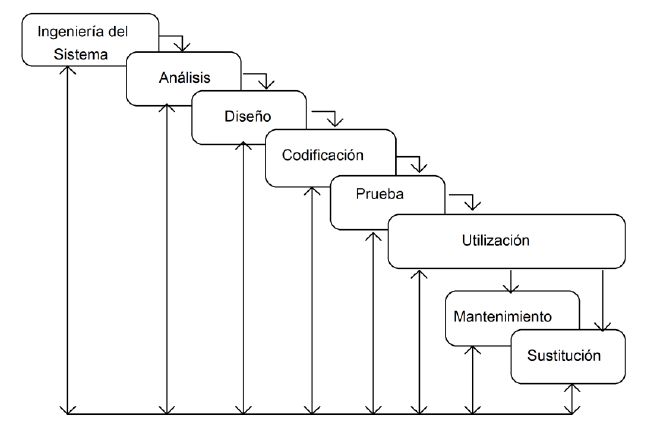
\includegraphics[width=0.7\linewidth]{Resources/cicloCascada}
  \caption{Etapas del ciclo de vida en cascada.}
  \label{fig:procesoCascada}
\end{figure}
 El ciclo de vida en cascada exige un enfoque sistemático y \textbf{secuencial} del desarrollo de software. Se dice que el modelo en cascada está guiado por documentos, ya que \textbf{nunca empieza la siguiente fase antes de que presente el documento de la anterior} (Tabla \ref{tab:cascadaDocumentos}).\\
 
\begin{table}[H]
\centering
\resizebox{\textwidth}{!}{%
\begin{tabular}{|l|l|}
\hline
\multicolumn{1}{|c|}{\textbf{Proceso}} & \multicolumn{1}{c|}{\textbf{Documentos Producidos}} \\ \hline
Especificaciones del sistema. & Especificación funcional. Arquitectura del sistema \\ \hline
Análisis de requisitos & Documento de requisitos \\ \hline
Diseño de la arquitectura del software & Especificación de la arquitectura \\ \hline
Diseño de interfaces & Especificación del diseño \\ \hline
Codificación & Código de programa \\ \hline
Prueba de unidades & Informe de pruebas de unidad \\ \hline
Prueba de módulos & Informe de pruebas de módulo \\ \hline
Prueba de integración & Informe de prueba de integración y manual de usuario final \\ \hline
Prueba del sistema & Informe de prueba del sistema \\ \hline
Prueba de aceptación & Sistema final más la documentación \\ \hline
\end{tabular}%
}
  \caption{Ejemplo de documentos producidos en un ciclo de vida en cascada. \textit{No tiene que tener exactamente las mismas fases que el ciclo en cascada por defecto.}}
  \label{tab:cascadaDocumentos}
\end{table}
 
 \subsection{Fases}
 \begin{enumerate}
 
     \item \textbf{Ingeniería y análisis del sistema}: Define las interrelaciones del software con otros elementos del sistema más complejo en el que esté englobado.
     
     \item \textbf{Análisis de requisitos del software}: Análisis detallado de los componentes del software incluyendo \textbf{datos} a manejar, \textbf{funciones} a desarrollar e \textbf{interfaces}.
     
     \item \textbf{Diseño}: \textbf{Estructura} de los datos, funciones, interfaces y aplicaciones.
     
     \item \textbf{Codificación}: Traducción del diseño a un formato que sea legible para la máquina. Produciendo un programa ejecutable.
     
     
     \item \textbf{Prueba}.
     
     \item \textbf{Utilización}.
     \item \textbf{Mantenimiento}.
     
     \begin{itemize}
         \item Errores latentes detectados por el cliente.
         \item Cambios en alguno de los componentes informáticos.
         \item Modificaciones funcionales requeridas por el cliente.
     \end{itemize}
 \end{enumerate}
 
 \subsection{Aportaciones}
 \begin{itemize}
    \item Es el más simple, conocido y fácil de usar.
    \item Los procesos definidos se \textbf{formalizan} en normas, \textit{sabes lo que tienes que hacer en cada momento}.
    \item Permite generar software eficiente, en el tiempo establecido en tiempo y forma (\textbf{funciona}).
    \item Al final de cada fase los interesados pueden comprobar el estado del proyecto.
 \end{itemize}
 
 \subsection{Problemas}
 \begin{itemize}
     \item En realidad el ciclo de vida \textbf{NO es secuencial}, ya que el \textbf{mantenimiento} y problemas con el proyecto exigen \textbf{volver atrás} a la parte donde se produjo el fallo. % 
     \item No siempre se pueden establecer los requisitos desde el primer momento. 
     \item Hasta que se llega a la fase final, no se dispone de una versión operativa del programa. 
     \item Los errores se detectan al final del proyecto, acentuando las pérdidas producidas por los fallos no detectados cometidos en fases anteriores.
 \end{itemize}
 
 \section{Ciclo de vida incremental} % Aquí la tipa se hecho un lío tremendo. Estaba todo mal.
% foto de incrementos
\begin{figure}[H]
  \centering
  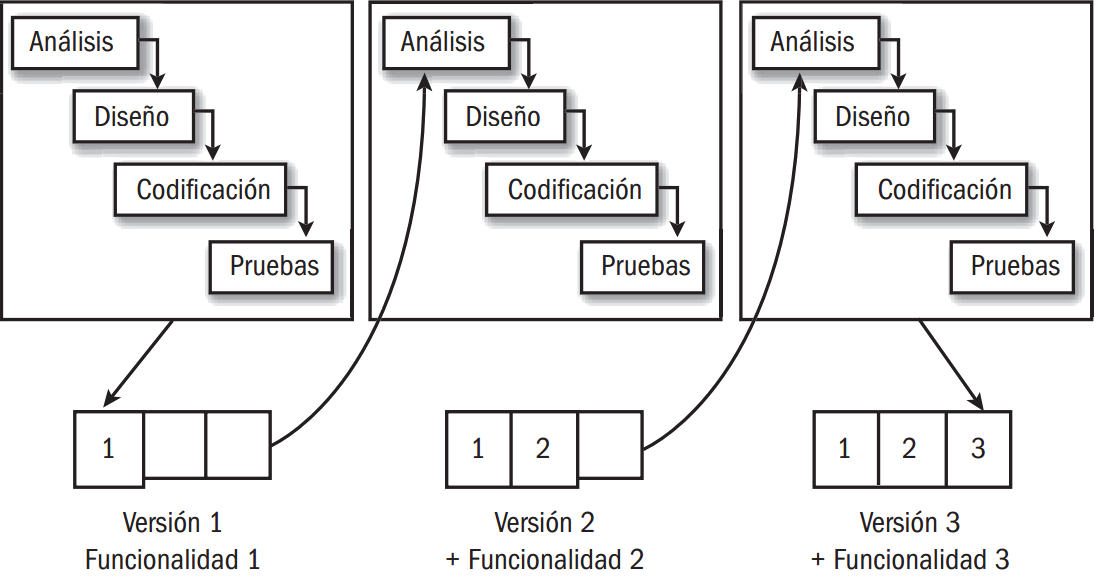
\includegraphics[width=0.7\linewidth]{Resources/cicloIncremental.png}
  \caption{Etapas del ciclo de vida incremental.}
  \label{fig:procesoIncremental}
\end{figure}

Surge como una \textbf{mejora del modelo en cascada} para paliar el problema de la \uline{detección de errores} y \uline{gestionar mejor los riesgos}.\\\\
Comenzamos como en cascada hasta la fase de diseño, completando solo el diseño preliminar. A partir de ahí separamos el proyecto en objetivos mas pequeños, que son \textbf{partes} del código \textbf{completas} y \textbf{funcionales} por sí mismas.\\\\
Para \textbf{cada incremento} realizamos las fases correspondientes de \textbf{diseño, codificación y explotación y mantenimiento}\footnote{A diferencia del resto de los mortales, Rabenso considera que el análisis no forma parte de los incrementos.}, obteniendo feedback.

\subsection{Ventajas}
%Tenemos por ahí el documento que hicimos de esto?
Soluciona parte de los problemas del modelo en cascada, mejorando la \textbf{comunicación con el cliente} y la \textbf{detección de errores} a tiempo.\\
Además, favorece la \textbf{modulación del software} al no pensarse como una unidad sino como la interacción de resultados sucesivos.\\

\subsection{Desventajas}
La parte de requisitos no se encuentra en la fase interactiva y por lo tanto tiene los problemas de cascada: es \textbf{difícil ver si los requisitos son válidos} y los \textbf{errores se detectan tarde}.





 \section{Construcción de prototipos}
 %Foto de ciclo prototipos
 \begin{figure}[H]
  \centering
  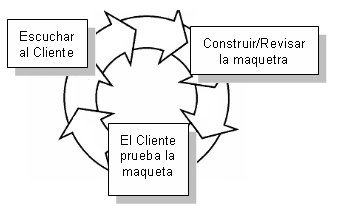
\includegraphics[width=0.7\linewidth]{Resources/construccionPrototipos.png}
  \caption{Etapas del paradigma de la construcción de prototipos.}
  \label{fig:construccionPrototipos}
\end{figure}

Consiste en la realización interactiva de prototipos hasta alcanzar un estado en el que los \textbf{requisitos} del sistema están \textbf{claros}, pasando entonces a desarrollar en cascada.\\


\subsection{Ventajas}

\begin{itemize}
    \item Muchas veces gran parte del \textbf{trabajo realizado} en los prototipos es \textbf{reutilizable}.
    \item En \textbf{proyectos con un nivel alto de incertidumbre}, donde los requisitos no están nada claros en primera instancia este ciclo provee un \textbf{método para obtener los requisitos de forma fiable} a través del feedback del usuario.
    \item Los prototipos permiten analizar \textbf{alternativas y viabilidades}. Refinando el resultado final o abortándolo antes de invertir demasiado dinero en el mismo.
\end{itemize}

\subsection{Problemas}
\begin{itemize}
   \item Es \textbf{posible que nunca se llegue a la fase de construcción}, lo cual da lugar a los problemas característicos de un software construido sin seguir procesos de ingeniería.
   \item Hay \textbf{mucha interacción con el cliente}, lo cual puede suponer un problema dependiendo de la predisposición del mismo a ver prototipos continuamente.
   \item Es imposible una \textbf{predicción de costes} fiable.
\end{itemize}



% Esto no recuerdo haberlo visto con Triñares. A mi me suena verlo muy de pasada
% Quizás lo que habría que hacer con esto es resumirlo en 10 líneas o menos.
\section{Técnicas de cuarta generación}
% yo creo que llega
% Sobra. Como mucho taboada pone una pregunta diciendo "son las técnicas de cuarta generación un desperdicio" o algo así.
%dejalo así Que son? y porque son mierda? no necesitas mas
Son un conjunto diverso de técnicas que permiten la generación de parte del código y la documentación; como el acceso a base de datos, interfaces gráficas e informes.\\\\
El mayor problema de estas técnicas es que el código que generan suele ser ineficiente y de menor calidad, requiriendo revisión y aumentando los costes de mantenimiento. Además no son fáciles de usar.\\\\ 
Sin embargo, a pesar de que no llegaron a conseguir los resultados esperados, reducen el tiempo y se utilizan sobre todo en software de gestión.


\section{Modelo en espiral}

%foto
 \begin{figure}[H]
  \centering
  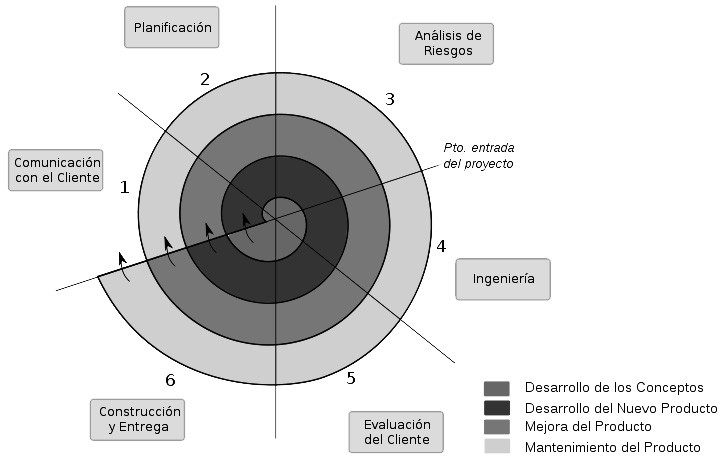
\includegraphics[width=0.7\linewidth]{Resources/modeloEspiral.jpg}
  \caption{Etapas del modelo en espiral.}
  \label{fig:modeloEspiral}
\end{figure}

Es un \textbf{modelo iterativo que combina las principales ventajas del modelo de ciclo de vida en cascada y el modelo de construcción de prototipos}. Del modelo en cascada sacamos la entrega de código ejecutable con funcionalidades válidas, estas entregas ahora son prototipos de la calidad requerida para cada fase habiendo pasado por fases previas de diseño.\\

    %Imagen del análisis de riesgos. La del magerit? trap 35 eso no es análisis, eso es administración del riesgo. Pero correcto
\subsection{Análisis de riesgos}
Este modelo incorpora, el análisis de riesgos basado en la identificación de amenazas a activos y el establecimiento de soluciones a esas amenazas (Administración de riesgos, Figura \ref{fig:administracionRiesgo}). Debemos pues:
\begin{enumerate}
   \item \textbf{Identificar los riesgos} Se identifican los activos, las amenazas y los riesgos potenciales (estimación del grado de exposición a que una amenaza se materialice en un activo). %tal cual los traparabas
   
   \item \textbf{Análisis de riesgos}: Estimación de la magnitud de los riesgos, obteniendo una lista de priorizanción de riesgos. 
   
   \item \textbf{Planificación de riesgos}: 
   Establecimiento de la estrategia adoptada contra el riesgo, pudiendo elegir entre:
   \begin{itemize}
      \item Estrategias de prevención.
      \item Estrategias de minimización.
      \item Planes de contingencia.
      % TODO aqui no falta transpaso, traspasar el riegos a otra empresa que lo gestione por ti?
   \end{itemize}
   \item \textbf{Gestión de riesgos}: Supervisar el desarrollo del proyecto, de forma que se detecten los riesgos tan pronto como aparezcan.
\end{enumerate}

\begin{figure}[H]
  \centering
  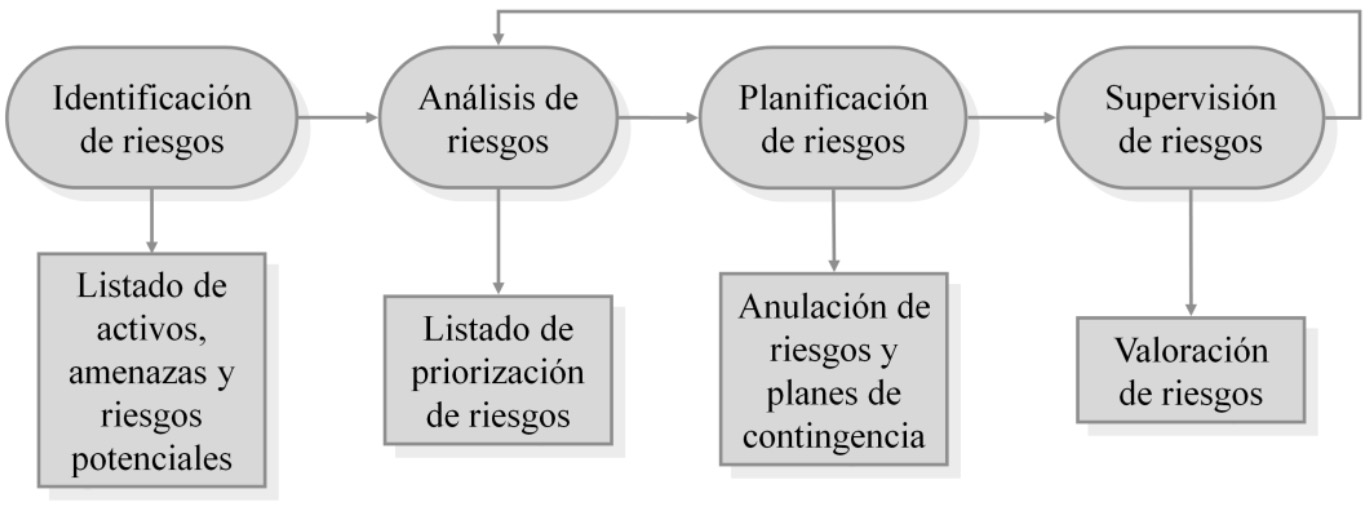
\includegraphics[width=0.7\linewidth]{Resources/administracionRiesgo.jpg}
  \caption{Administración del riesgos.}
  \label{fig:administracionRiesgo}
\end{figure}

% Esto que quieres hacer, un nuevo subsection? zumbale. Las imágenes han sido todas cambiadas a blanco y negro, mejorado el contraste para la hora de imprimir y limpiado si tenían manchas porque rabenso no sabe escanear.

\subsection{Descripción del modelo}
El modelo en espiral define 4 tipos de actividades de las que consta un ciclo:
\begin{enumerate}
   \item \textbf{Definición de objetivos}.
   \item \textbf{Análisis de riesgos}.
   \item \textbf{Desarrollo y validación}.
   \item \textbf{Revisión y planificación}: En ella se decide si se continúa con el proyecto o no, y se realizan planes para el siguiente ciclo.
\end{enumerate}



\subsection{Ventajas}% deducir, no las dice explícitamente
\begin{itemize}
   \item Entrega de prototipos con la calidad requerida para cada fase de código ejecutable con funcionalidades básicas válidas.
   \item Incorporación del análisis de riesgos.
\end{itemize}

\subsection{Desventajas}
\begin{itemize}
   \item Es difícil de adaptar a un contrato, aunque se puede utilizar el modelo de contrato por iteración.
   \item Requiere habilidad en la gestión de riesgos.
   \item Un riesgo no detectado a tiempo es similar a un requisito no detectado a tiempo. %no se porqué eso es un incomveniente pero rabo
   \item Requiere muchos recursos para su control, y es difícil convencer al cliente de que lo estás controlando.
\end{itemize}

\section{Metodologías ágiles}
% RRHH  meets RABENSO

%Sorprendente estos dos párrafos están bien.
El desarrollo ágil defiende la renuncia a utilizar modelos perfectos, se basa únicamente en que sean lo suficientemente buenos. Tratan de \textbf{centrar los esfuerzos en presentar un incremento software ejecutable}, restando importancia a los productos de trabajo intermedio.
\\\\
Los \textbf{incrementos son valorados por el cliente}, que entra de forma efectiva en el proceso desarrollo del software y ofrece la necesaria realimentación al equipo de desarrollo.
\\\\
Las metodologías pesadas se enfrentan a las limitaciones de las personas que intervienen en los procesos, mientras que las metodologías ligeras adoptan un \textbf{enfoque de tolerancia donde el modelo se adapta al equipo} y no a la inversa.

\subsection{Equipo ideal para las metodologías ágiles}
Debe buscarse un equipo con los siguientes rasgos (que suenan a algo que diría un \textit{young business entrepreneur}):
\begin{itemize}
   \item \textbf{Competencia} sobre el proceso.
   \item \textbf{Enfoque común}, la meta es la entrega rápida.
   \item \textbf{Colaboración} entre stakeholders.
   \item \textbf{Habilidad para la toma de decisiones}, necesaria para una entrega rápida.
   \item \textbf{Capacidad de resolución de problemas confusos} ante la no concreción de requisitos.
   \item \textbf{Confianza y respeto mutuo}. %NO cuernos joder
   \item \textbf{Capacidad de autoorganización}. %Ala
\end{itemize}

\paragraph{Principios para alcanzar la agilidad}

\begin{enumerate}
    \item La mayor prioridad es \textbf{satisfacer al cliente} mediante la entrega temprana y continua de software valioso.
    \item Bienvenidos los \textbf{requisitos cambiantes}, incluso en fases tardías del desarrollo.
    \item \textbf{Entregar con frecuencia} software en funcionamiento.
    \item La \textbf{gente de negocios} y los \textbf{desarrolladores} deben \textbf{trabajar juntos} a diario. % Reunión Reunión Reunión! Reunión Reunión Reunión!
    \item Construir \textbf{proyectos alrededor de individuos motivados}. Darles el ambiente y soporte necesario que necesitan, y confiar en ellos para obtener el trabajo realizado. % MOTÍVATE
    \item El método más eficiente y efectivo para transmitir información es la \textbf{conversación cara a cara}.
    \item \textbf{El software en funcionamiento es la medida primaria de progreso}.
    \item Los procesos ágiles promueven el \textbf{desarrollo sostenible}. %Porque lo dices tú
    \item La atención continua a la excelencia técnica y al buen diseño mejora la agilidad.
    \item La simplicidad es esencial. %Por eso ponemos 12 principios.
    \item Las mejores arquitecturas, los mejores requisitos y los mejores diseños emergen de \textbf{equipos autoorganizados}.
    \item A intervalos regulares el \textbf{equipo refleja} la forma en que se puede \textbf{volver más efectivo}.
\end{enumerate}
%Puedo poner algo en lo de los equipos?

\subsection{Modelado ágil}
A \textbf{alto nivel} es una \textbf{colección de buenas prácticas}, entrando \textbf{en detalle} es una \textbf{colección de valores}, principios y practicas. Puede ser tomado más como una filosofía que como una metodología: 
\begin{itemize}
   \item Modelar con un propósito.
   \item Usar múltiples modelos.
   \item Viajar ligero: Conservar sólo los modelos que proporcionarán valor a largo plazo.
   \item El contenido es más importante que la representación.
   \item Conocer los modelos y herramientas con que se crean.
   \item Adaptar al equipo ágil.
\end{itemize}

\subsection{Programación extrema}
 \begin{figure}[H]
  \centering
  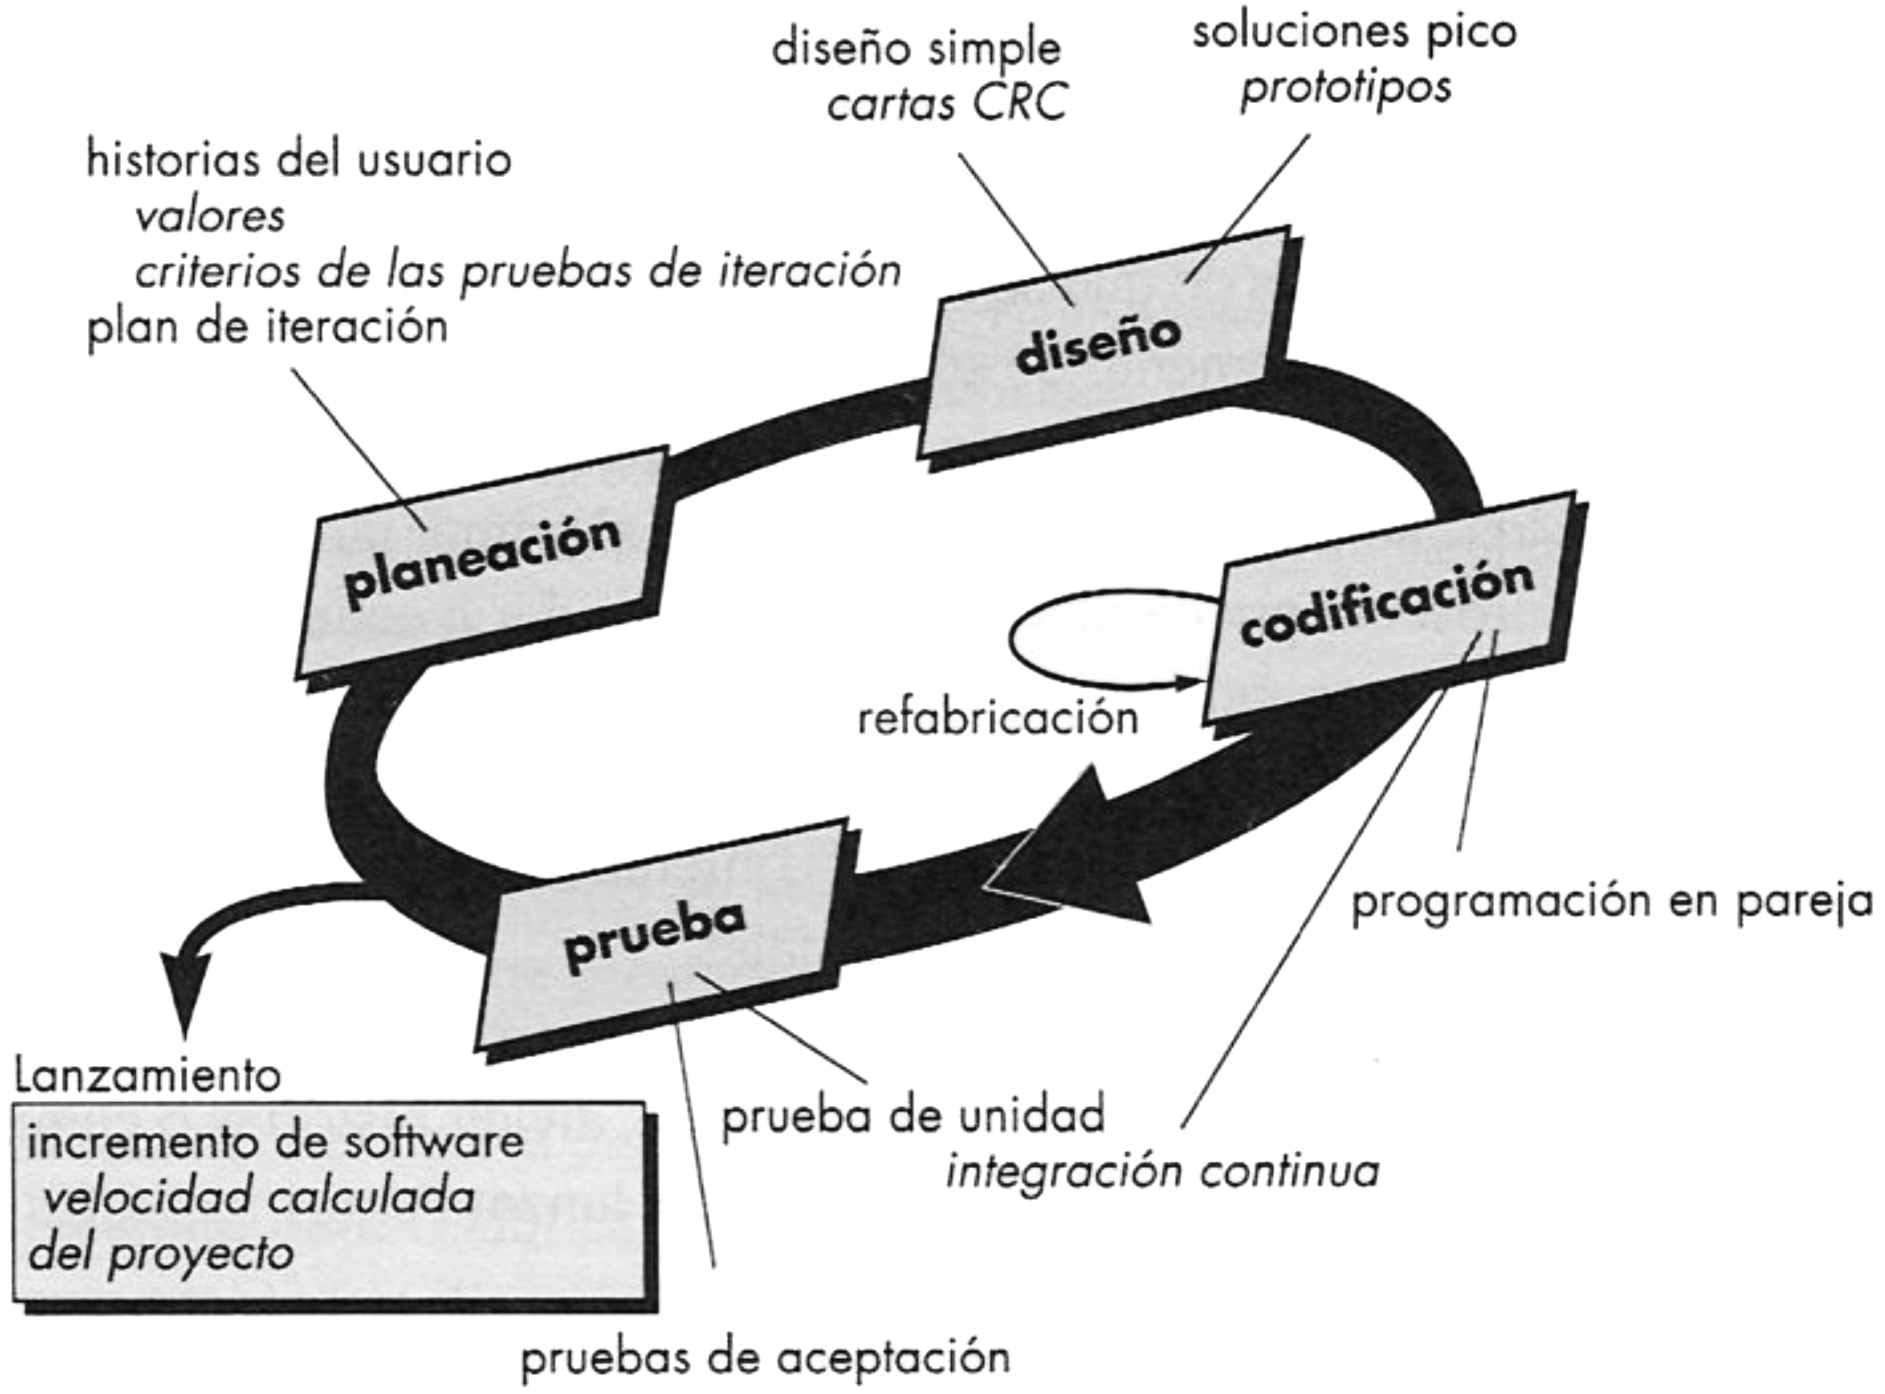
\includegraphics[width=0.7\linewidth]{Resources/programacionExtrema.jpg}
  \caption{Etapas de la programación extrema.}
  \label{fig:programacionExtrema}
\end{figure}
% Venga lo dejo
\textbf{Utiliza un enfoque orientado a objetos}: Abarca un conjunto de reglas que ocurren en el contexto de las siguientes actividades:
\begin{enumerate}

    \item \textbf{Planificación}:
    \begin{itemize}

       \item \textbf{Creación de historias de usuario}: Utiliza historias de usuario para establecer los requisitos, a las que se el usuario asigna un valor de prioridad.
       \item \textbf{Estimación del tiempo de implementación}: Si es superior a 3 semanas se reescribe la historia.
       
       \item \textbf{Plan de construcción}: Los clientes y el equipo se reúnen para decidir qué historias hay en el siguiente incremento, priorizando de la siguiente forma:
       \begin{itemize}
          \item Todas las historias serán implementadas de un modo inmediato.
          \item Las historias con \textbf{valor más alto} se moverán en el programa y se implementarán al \textbf{principio}.
          \item Las historias de \textbf{mayor riesgo} se moverán en el programa y se implementarán al \textbf{principio}.
       \end{itemize}
       Después de que se haya entregado el primer lanzamiento, se calcula la \textbf{velocidad del proyecto}, que es el número de historias del cliente implementadas en el primer lanzamiento. 
       
       La velocidad se puede usar para ayudar a estimar fechas de entrega o determinar si se ha hecho un compromiso excesivo en algunas historias, en cuyo caso se modifica el contenido de los lanzamientos o se cambian las fechas de entrega.
          
    \end{itemize}
    
    
   \item \textbf{Diseño}: Sigue el principio KISS (\textit{Keep It Simple, Stupid}) y se apoya en: 
   % https://en.wikipedia.org/wiki/KISS_principle El stupid es importante. Porque somos estúpidos y debemos recordarlo.
   \begin{itemize} %Mejor así.
      \item \textbf{Tarjetas CRC} (Colaborador--Responsabilidad--Clase). 
      \item \textbf{Prototipado}: Para la resolución de problemas difíciles, se recomienda construir prototipos.
      \item \textbf{Prefabricación}: Nos apoyamos en mejorar la estructura interna del software sin que se altere el comportamiento externo.
      \item \textbf{Diseño como artefacto}: Se permite la modificación del diseño durante la construcción.
   \end{itemize}

   \item \textbf{Codificación}: Se prefiere crear las \textbf{pruebas antes que el código} de las clases.
   
   \item \textbf{Pruebas}: Se distinguen:
   \begin{itemize}
      \item \textbf{De unidad}: realizadas a diario y a ser posible, de forma automatizada para evitar que los problemas se vuelvan enormes.
      \item \textbf{De aceptación}: especificadas por el cliente, enfocadas a características generales y de funcionalidad del sistema que el cliente puede revisar. %Lo de que son elementos visibles y revisables por el cliente es redundante.
   \end{itemize}
% Los temas van a peor el 4, 5 y 6 están muy intratablesTM.
\end{enumerate}

\newpage
\part{Análisis de requisitos}
\section{Introducción}

\subsection{Requisito}
 Condiciones o capacidades de debe cumplir un sistema para satisfacer un contrato, norma o especificación.
 
\subsubsection{Clasificación de los requisitos}
\begin{itemize} % Para llamarlos así mejor requisitos declarativos, restrictivos y de dominio... estan como el rabo quiere
    \item \textbf{Requisitos funcionales}: Declaraciones de los servicios o funcionalidades que implementará el sistema. \textit{Ejemplo: El usuario tendrá la posibilidad de buscar por tamaño}.
    
    \item \textbf{Requisitos no funcionales}: Restricciones sobre los servicios o funciones ofrecidos por el sistema. Pueden ser temporales, de fiabilidad, robustez, de ajuste a estándares\ldots\\
    Deben expresarse de forma cuantitativa. 
    \textit{Ejemplo: La duración de la sesión ha de ser superior a 30 minutos}.
    
    \item \textbf{Requisitos del dominio}: Provienen del entorno en el que se realiza la aplicación y pueden ser funcionales o no funcionales. \textit{Ejemplo: usar el formato DICOM en medicina es a la vez un requisito no funcional y de entorno}.
\end{itemize}

\subsection{Análisis de requisitos}

Proceso de \textbf{estudio de las necesidades de los usuarios} para llegar a una definición de los requisitos obtenidos, incluyendo el proceso de refinamiento de los mismos.
\\\\
Encontramos este proceso en todos los modelos de ciclos de vida, compartiendo las siguientes características comunes:
\begin{enumerate}
    \item Realizan una abstracción de las características del sistema.
    \item Representan el sistema de forma jerárquica.
    \item Definen las interfaces del sistema, tanto externas como internas. %definen las interfaces internas entre modulos pero en esta fase todavía no se crearon módulos, bien rabenso.
    \item Sirven de base para etapas posteriores del diseño e implementación.
    \item Se plantean por niveles: usuario, de sistema, esenciales y de implementación.
    \item No prestan demasiada atención a la representación de las restricciones o criterios de validación. (excepto los métodos formales).
\end{enumerate}

\textit{Rabenso dice: Por norma general, se debería dedicar un 40\% del tiempo de desarrollo de un proyecto al análisis y diseño, un 20\% a la codificación, y un 40\% a la fase de pruebas.}

\subsection{Personal implicado}

\begin{enumerate}
\item \textbf{Analista}: Es el encargado de la comunicación con los stakeholders y los desarrolladores, sirviendo de puente entre ambos. Para este labor debe de tener conocimiento multidisciplinar, buenas dotes de comunicación y ser capaz de traducir ideas vagas de necesidades de software en un conjunto concreto de funciones y restricciones.

\item \textbf{Stakeholders}: personal involucrado en el proyecto, incluyendo a los usuarios finales, los ingenieros trabajando en el proyecto, el administrador de negocio y los expertos del dominio del sistema. Podemos distinguir entre involucrados y comprometidos.
\end{enumerate}


\subsection{Razones por las que el análisis de requisitos es difícil}
\textit{Sommerville} establece las siguientes razones:
\begin{itemize}
    \item Los stakeholders a menudo no conocen realmente lo que desean obtener del sistema.
    \item Los stakeholders expresan los requisitos con sus propios términos. Los ingenieros de requisitos deben comprenderlos.
    \item Diferentes stakeholders tienen requisitos distintos que expresan de varias formas. Los ingenieros de requisitos tienen que descubrir todas las fuentes potenciales de requisitos así como las partes comunes y en conflicto.
    \item Puede haber condicionantes políticos y de la organización.
    \item El entorno económico y de negocios en el que se lleva a cabo el análisis es dinámico, y cambia durante el proceso de análisis, por lo que la importancia de ciertos requisitos puede cambiar.
\end{itemize}


\section{Obtención de requisitos} %Sigamos la convención del rabenso
El proceso de análisis de requisitos tiene las siguientes fases:
\begin{itemize}
    \item \textbf{Identificar las fuentes de información} relevantes para el proyecto.
    \item \textbf{Realizar las preguntas apropiadas} para comprender sus necesidades.
    \item \textbf{Analizar la información recogida} para detectar aspectos poco claros.
    \item \textbf{Confirmar con los usuarios} lo que se ha comprendido de los requisitos.
    \item \textbf{Sintetizar los requisitos} en un documento de especificación apropiado.
\end{itemize}

\subsection{Técnicas de comunicación y recogida de información}
Aparecen a raíz de uno de los problemas más comunes: cómo poner en contacto a usuarios y técnicos para establecer unos requisitos entendibles y aceptados por todos.
%voy a borrar las definiciones de esto que sean trivilaes
\begin{enumerate}
    \item \textbf{Entrevistas}.
    \item \textbf{Desarrollo conjunto de aplicaciones}: Se crean equipos de usuarios y analistas que determinan conjuntamente las características que debe tener el software. \textit{Ejemplo TFEA}.
    \item \textbf{Prototipado}.
    \item \textbf{Observación}: Consiste en analizar \textit{in situ} cómo funciona la unidad o el departamento a informatizar.
    \item \textbf{Estudio de documentación}: recopilar muestras de los impresos que se utilizan en la organización.
    \item \textbf{Cuestionarios}.
    \item \textit{\textbf{Brainstorming}}: Consiste en reuniones de entre 4 y 10 personas en las que se sugiere toda clase de ideas \uline{sin juzgarse su validez}, para luego analizar cada propuesta de modo detallado.
    \item \textit{\textbf{Casos de uso}}.
\end{enumerate}
%La mitad de este párrafo es trivial.todo es trivial xD. pues al pozo.

\subsection{TFEA}
%Poner que cona significan las siglas de TFEA -> en inglés no era FAST? No costaba tanto poner las cosas claras EH RABENSO.
Son un conjunto \textbf{T}écnicas de \textbf{F}acilitación de \textbf{E}specificación de la \textbf{A}plicación.
\begin{enumerate}
   \item Redacción de un documento inicial como resultado de reuniones entre analista y cliente:
\begin{enumerate}[a.]
    \item Descripción del problema.
    \item Objetivos.
    \item Propuesta de solución (si es posible).
\end{enumerate}
\item Creación de listas individuales de:
    \begin{enumerate}[a.]
        \item Objetos del sistema y del entorno.
        \item Operaciones que relaciones objetos.
        \item Restricciones.
        \item Rendimiento.   
    \end{enumerate}
\item Creación de una lista conjunta a partir de las individuales, sin eliminar nada.
\item Discusión de la lista conjunta (deben estar representados el analista, el cliente y el equipo de desarrollo).
\item Redacción de miniespecificaciones.
\item Redacción de un borrador de la especificación.
\end{enumerate}
Este enfoque presenta numerosas ventajas, como la comunicación multilateral de todos los involucrados en el proyecto, el refinamiento instantáneo y en equipo de los requisitos y la obtención de un documento de base para el proceso de análisis. 


\section{Análisis de requisitos} 

\subsection{Análisis de requisitos del sistema}

El objetivo es \textbf{conseguir representar un sistema en su totalidad}, incluyendo hardware, software y personas, mostrando la relación entre diversos componentes y \textbf{sin entrar en la estructura interna} de los mismos.\\\\
El análisis de sistemas tiene las siguientes fases:
\begin{enumerate}
    \item \textbf{Identificación de las necesidades del cliente}:\\
    Recogida y clasificación de requisitos. Distinguimos entre:
    \begin{itemize}
        \item Requisitos prescindibles e imprescindibles.
        \item Requisitos normales, esperados e estimulantes (lo que el cliente pide, lo que el cliente necesita y los que le resultarían satisfactorios respectivamente). %estoy dudando si poner el ejemplo del rabo
    \end{itemize} %es un ejemplo larguísimo
    % DAFO: Debilidades, Amenazas, Fortalezas y Oportunidades
    \item \textbf{Análisis de alternativas}:\\ Estudio de las diferentes alternativas que solucionen el problema o parte de él, incluyendo las ya implementadas por terceros. Para ello podemos utilizar técnicas como el \textbf{análisis paramétrico}, diagramas \textbf{DAFO} (Debilidades, Amenazas, Fortalezas y Oportunidades) o el \textbf{valor monetario esperado} (EMV).
\begin{table}[h]
    \centering
    \resizebox{0.75\textwidth}{!}{%
    \begin{tabular}{l|l|l|l|}
    \cline{2-4}
    \multicolumn{1}{c|}{\textbf{}} & \multicolumn{1}{c|}{\textbf{Alternativa 1}} & \multicolumn{1}{c|}{\textbf{Alternativa 2}} & \multicolumn{1}{c|}{\textbf{Alternativa 3}} \\ \hline
    \multicolumn{1}{|l|}{Inversión inicial} & Nula & Moderada & Grande \\ \hline
    \multicolumn{1}{|l|}{Coste funcionamiento} & Grande & Moderado & Moderado \\ \hline
    \multicolumn{1}{|l|}{Tiempo amortización} & Nulo & Moderado & Grande \\ \hline
    \multicolumn{1}{|l|}{Fiabilidad} & Moderada & Pequeña & Grande \\ \hline
    \multicolumn{1}{|l|}{Mantenimiento} & Nulo & Grande & Moderado \\ \hline
    \multicolumn{1}{|l|}{Flexibilidad} & Alta & Nula & Alta \\ \hline
    \end{tabular}%
    }
    \caption{Análisis paramétrico de un sistema de clasificación de paquetes.}
    \label{tab:analisisParametrico}
\end{table}

\begin{figure}[H]
  \centering
  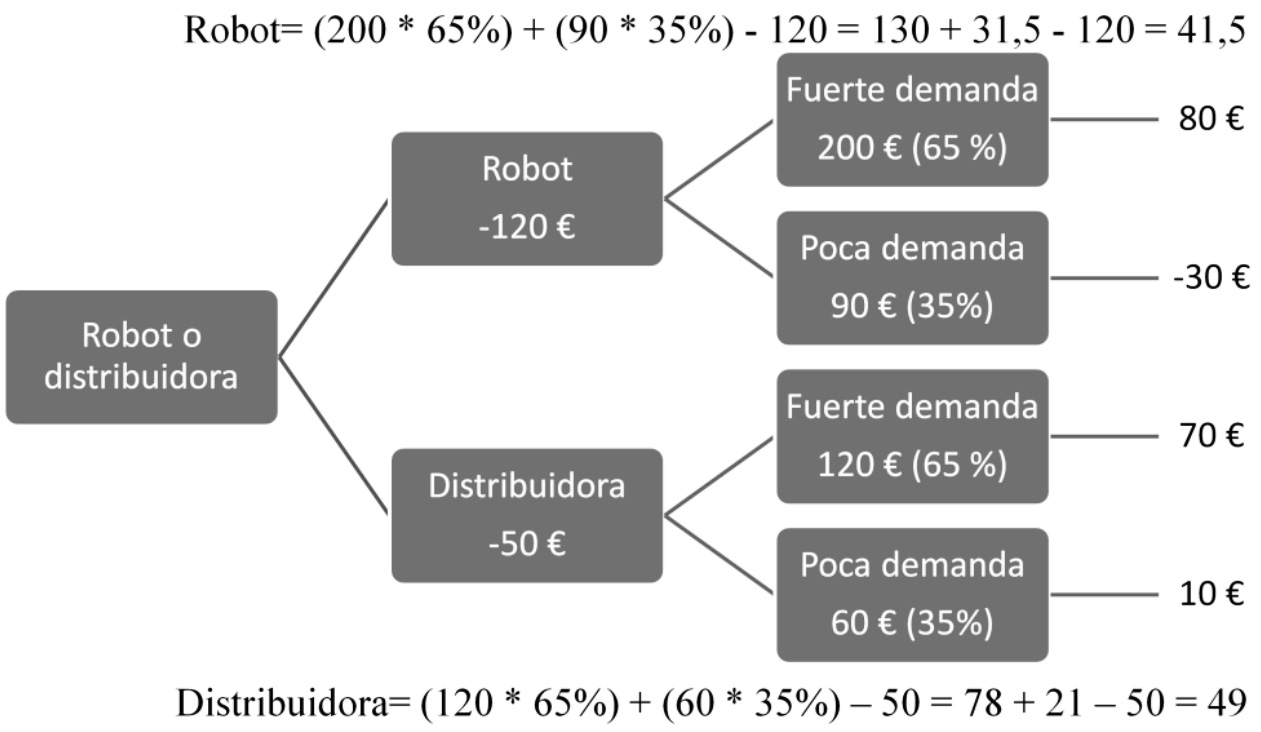
\includegraphics[width=0.7\linewidth]{Resources/emv}
  \caption{EMV de un sistema de clasificación de paquetes.}
  \label{fig:emv}
\end{figure}
    
    
    \item \textbf{Estudio de viabilidad del sistema}:\\
    Pretende determinar si merece la pena la construcción del software: si el sistema puede implantarse con las restricciones de coste y tiempo con la tecnología actual y con un alcance que le sea útil al usuario.\\
    Para ello se hace un estudio de viabilidad desde el punto de vista económico, técnico, legal, operativo y de plazos.
    \begin{figure}[H]
        \centering
        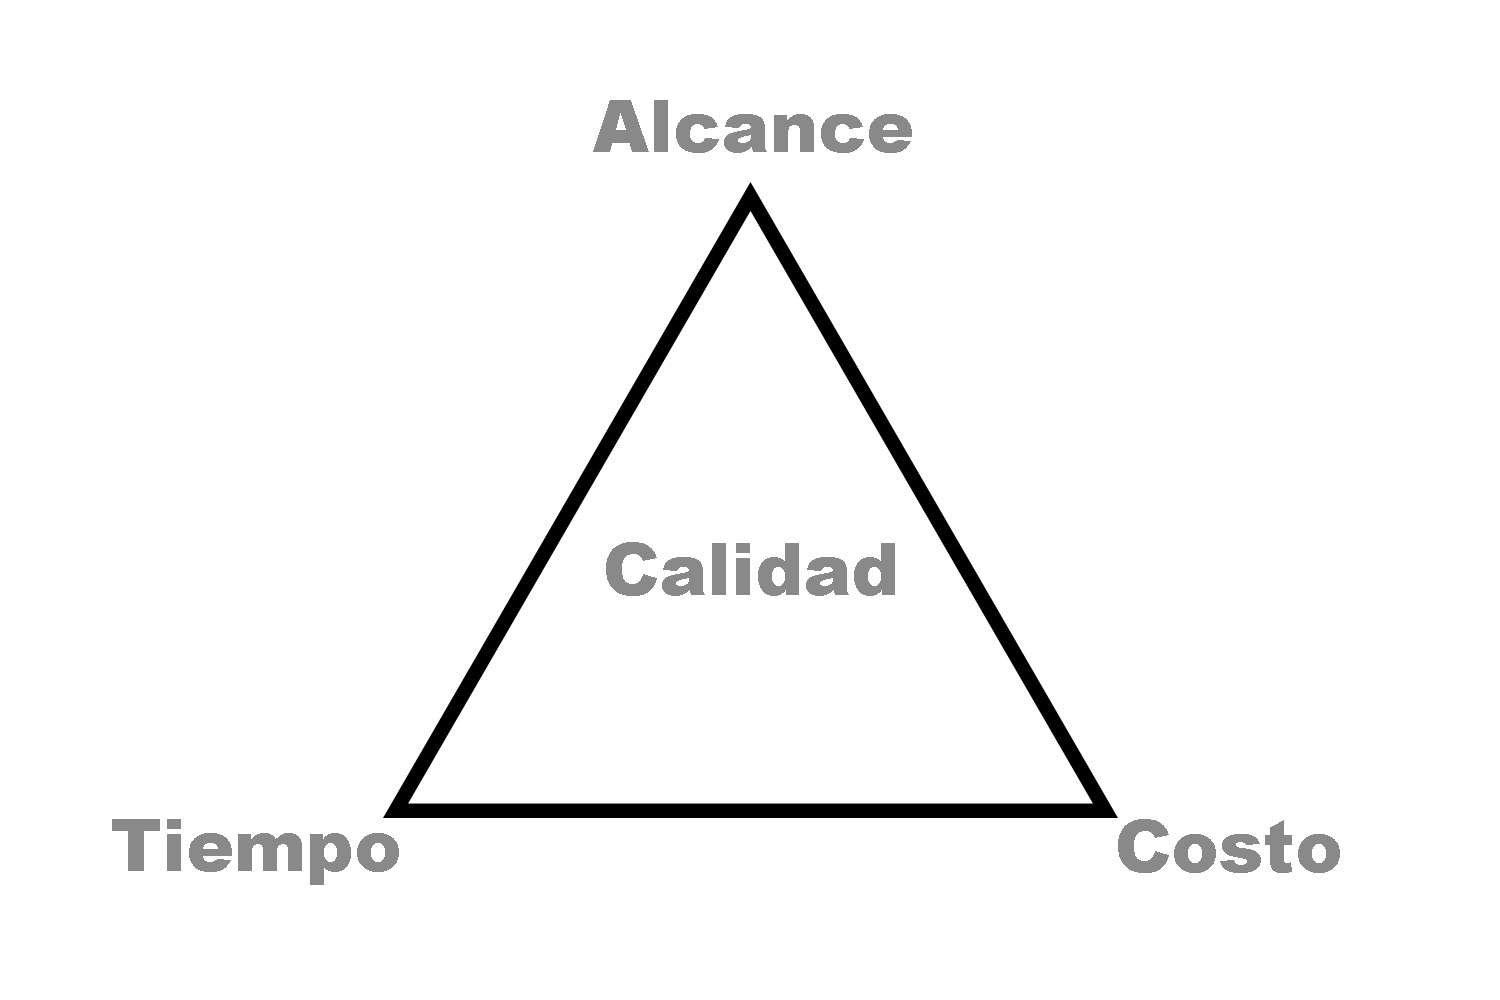
\includegraphics[width=0.4\linewidth]{Resources/PMI}
        \caption{La calidad del software está restringida en mayor medida, pero no únicamente por el tiempo, el coste y el alcance.}
        \label{fig:PMI}
    \end{figure}
    
    \item \textbf{Definición del sistema para que sea la base del trabajo posterior}: Para ello tenemos los siguientes diagramas:
    \begin{itemize}
        \item \textbf{Diagrama de contexto}: Representa el sistema en relación con su entorno. Define los límites del sistema y muestra todos los productores y consumidores de información. El sistema se relaciona con los agentes externos mediante flujos de información.\\
        \textit{Pressman} recomienda realizar este diagrama separado en secciones: Entrada, Salida, interfaz de usuario, función y control de sistema y mantenimiento y diagnóstico.
        \begin{figure}[H]
        \centering
        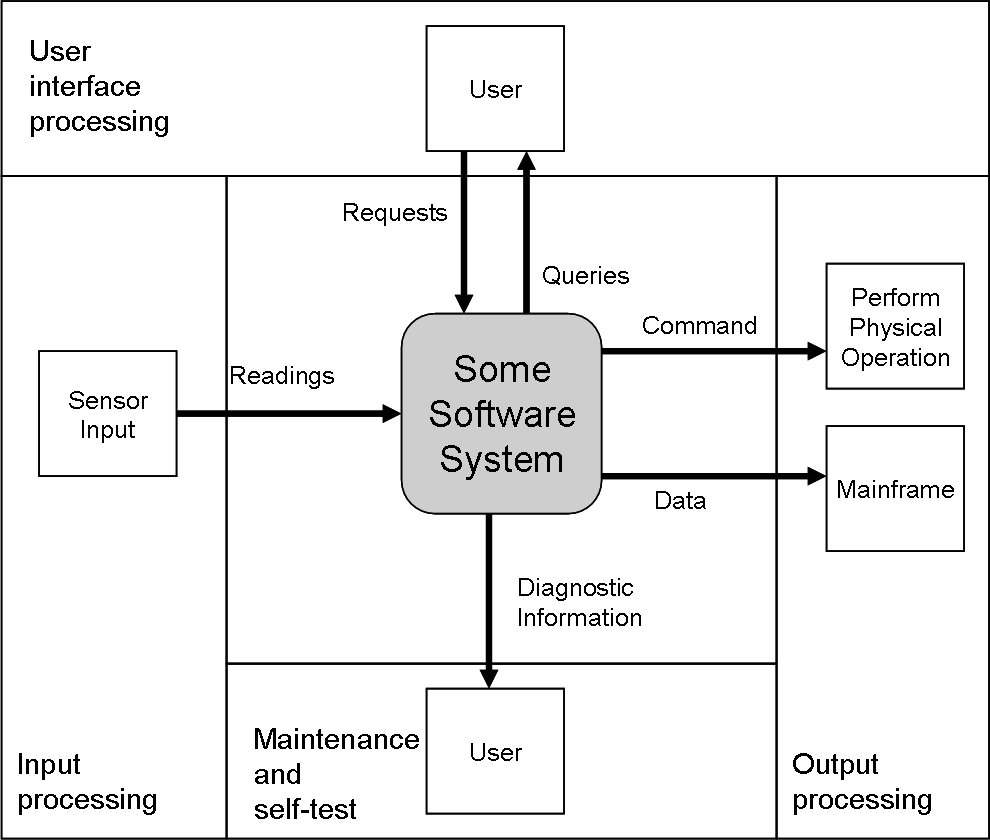
\includegraphics[width=0.5\linewidth]{Resources/contextdiagram}
        \caption{Ejemplo de diagrama de contexto siguiendo la plantilla.}
        \label{fig:diagramaDeContexto}
    \end{figure}
        \item \textbf{Diagrama de flujo}: Determinan el flujo de entre los diferentes subsistemas a través de diagramas de flujo convencionales.
    \end{itemize}
\end{enumerate}.


% Inicio de la zona que o aparece en los apuntes del rabens
\subsection{Análisis de requisitos del software}

El análisis de requisitos del software tiene como objeto\textbf{ desarrollar una representación del software que pueda ser revisada y aprobada por el cliente} que permitirá valorar la calidad del software una vez construido.
\\\\
Desde el punto de vista del analista, esta fase define con mayor precisión las funciones y rendimiento del software, las interfaces con otros componentes y las restricciones que debe cumplir. 

\subsubsection{Principios del análisis de requisitos del software}
\begin{enumerate}
    \item \textbf{Identificar y representar el ámbito de información del sistema}: La tarea que realiza el software consiste en procesar información, representada tanto por \textbf{datos} como por \textbf{sucesos o eventos}. El ámbito de información admite dos puntos de vista: flujo de datos y flujo de control.
    \item \textbf{Modelar la información, la función y el comportamiento del sistema}: Se emplean \textbf{modelos de datos} (información que transforma el software), \textbf{modelos de procesos} (procesos que transforman la información) y \textbf{modelos de control} (comportamiento del sistema).\\
    Utilidades de los modelos:
    \begin{itemize}
        \item Ayudan al analista a entender la información, función y comportamiento del sistema.
        \item Sirven de base para el trabajo del diseñador.
        \item Sirven para validar el producto una vez desarrollado.
    \end{itemize}
    \item \textbf{Descomponer el problema de forma que se reduzca la complejidad.}
    \item \textbf{Avanzar desde lo más general a lo más detallado.}
\end{enumerate}
% Fin de la zona que no aparece en los apuntes del rabenso


\section{Especificación}

\subsection{Especificación del sistema} 
Documento que describe la función, rendimiento y restricciones que el sistema debe cumplir, limitando cada uno de sus componentes.\\

Es labor del analista realizar una \uline{evaluación inicial}, determinando si:
\begin{enumerate}
     \item Se ha delimitado correctamente el ámbito.
     \item Se han definido correctamente las funcionalidades, el comportamiento, las interfaces y el rendimiento.
     \item Las necesidades de usuario y el análisis de viabilidad justifican el desarrollo del proyecto.
     \item Las percepciones acerca del objetivo del proyecto del cliente y el analista coinciden.
\end{enumerate}
El analista deberá hacer además una \uline{evaluación técnica}, comprobando:
\begin{enumerate}
    \item Todos los detalles técnicos están bien definidos.
    \item La especificación sirve como base para las siguientes fases.
    \item Las estimaciones de riesgos, tiempos y costes se corresponden con la complejidad del proyecto.
\end{enumerate}


\subsection{Especificación del software} 
Documento que define, de forma completa, precisa y verificable, los requisitos, el diseño, el comportamiento u otras características de un sistema o componente del mismo.\\
Es el documento que culmina el análisis de requisitos, conteniendo:
\begin{enumerate}
    \item Descripción detallada del ámbito de información.
    \item Funciones y comportamiento asignados al software.
    \item Restricciones de rendimiento y diseño.
    \item Pruebas de aceptación.
\end{enumerate}


% % \subsection{Especificación de requisitos}
% % Documento que define de forma completa, precisa y verificable, los requisitos, el diseño, el comportamiento u otras características del sistema o un componente del mismo.\\\\
% Debe contener una descripción detallada del ámbito de información, las funciones, el comportamiento del software, los requisitos de rendimiento y restricciones de diseño, y sobre las pruebas que se realizarán al software una vez construido.
\subsubsection{Principios de especificación}
\begin{enumerate}
    \item Debe modelar el dominio del problema.
    \item Es necesario separar funcionalidad e implementación.
    \item El lenguaje de especificación debe estar orientado al proceso.
    \item Debe abarcar todo el sistema del que el software es parte.
    \item Debe abarcar también el entorno del sistema.
    \item La especificación debe ser operativa.
\end{enumerate}

\subsubsection{Características del documento de especificación}

\begin{enumerate}
    \item \textbf{Preciso}: Cada requisito debe tener una única interpretación. Evitar el lenguaje natural.
    \item \textbf{Completo}: Una especificación de requisitos software (ERS) está completa si:
    \begin{itemize}
        \item Incluye todos los requisitos significativos del software.
        \item Define la respuesta software a todas las entradas en todas las situaciones.
        \item Está conforme con cualquier estándar de especificación que se deba cumplir.
        \item Están etiquetadas y referenciadas todas las tablas, figuras y diagramas del texto, y están definidos todos los términos y unidades de medida.
        \item No contiene la expresión \textit{TBD} (por determinar). A veces es necesario utilizarla, y debe acompañarse de:
        \begin{itemize}
            \item Una descripción de las condiciones que han causado el \textit{TBD}.
            \item Una descripción de qué hay que hacer para eliminar el \textit{TBD}.
        \end{itemize}
    \end{itemize}
    \item \textbf{Fácil de verificar}. Cualquier requisito al que hace referencia se puede verificar mediante algún procedimiento finito y efectivo en coste.
    \item \textbf{Consistente}: %Se entiende que es la especificación del software porque estamos hablando de eso XD
    \begin{itemize}
        \item Ningún conjunto de requisitos descritos en la especificación deben describir el mismo objeto real pero utilizar distintos términos para designarlo.
        \item Las características especificadas de objetos reales no pueden estar en conflicto.
        \item Ningún conjunto de acciones determinadas deben entrar en conflicto lógico o temporal.
    \end{itemize}
    \item \textbf{Fácil de modificar}.

    \item \textbf{Facilidad para identificar el origen y las consecuencias de cada requisito}: se consigue estableciendo la trazabilidad.
    
    \item \textbf{Facilidad de utilización durante la fase de explotación y mantenimiento}. %osea el REM no

\end{enumerate}





\section{Verificación y Validación de requisitos}
\subsection{Estrategias}
Encontramos diferentes estrategias para la verificación y validación de requisitos:
\begin{enumerate}
    \item \textbf{Comprobación de validez}. ¿Responde a todas las necesidades?
    \item \textbf{Comprobación de consistencia}. ¿Hay incongruencias en los requisitos? % XD
    \item \textbf{Comprobación de totalidad}. ¿Nos falta algo por especificar? 
    \item \textbf{Verificaciones de realismo}. ¿Es posible implementar la funcionalidad requerida?
    \item \textbf{Verificabilidad}. ¿Soy capaz de crear pruebas que determinen si se pasa cada requisito?
\end{enumerate}

\subsection{Técnicas}
Existen varias \uline{técnicas de validación} de requisitos:

\begin{enumerate}
    \item \textbf{Revisiones de requisitos} Proceso manual de verificación del documento de requisitos que busca encontrar anomalías y omisiones.%por grupos de revisores %Los requisitos son analizados por un grupo de revisores.
    \item \textbf{Construcción de prototipos}. %Se muestra un modelo ejecutable del sistema a los usuarios finales para que experimenten con él.
    \item \textbf{Generación de casos de prueba}. Los requisitos deben poder probarse. Si una prueba es difícil o imposible de diseñar, suele significar que los requisitos serán difíciles de implementar, por lo que deben ser reconsiderados.
    \item \textbf{Análisis de consistencia automática}. Si los requisitos se expresan como un modelo del sistema en una notación estructurada o formal, las herramientas CASE(Computer Aided Software Engineering) deben verificar la consistencia del modelo.
\end{enumerate}
% aparte esta arriba
% Estaba en el enumerate mencionado (porque así lo tiene rabenso), no creo que quiera que sepamos mucho del tema hay bastantes más cosas importantes que las clasificaciones de las revisiones de requisitos/
\section{Administración de requisitos}
La especificación de requisitos es un proceso iterativo, por lo tanto hace falta un proceso formal para gestionar la realización de modificaciones a los requisitos sin descuidar la calidad de la documentación de requisitos.\\
Para ello debemos llevar a cabo un registro de modificaciones

\subsection{Clasificación cualitativa}
\begin{enumerate}
    \item \textbf{Requisitos duraderos}
    \item \textbf{Requisitos volátiles}
    \begin{itemize}
        \item \textbf{Cambiantes}: Cambian debido a los cambios en el ambiente en que opera la organización. 
        \item \textbf{Emergentes}: Surgen al incrementar la comprensión del cliente en el desarrollo del sistema.
        \item \textbf{Consecutivos}: Son resultado de la introducción del sistema de cómputo. %valla nombre de mierda
        \item \textbf{De compatibilidad}: Dependen de sistemas particulares o procesos de negocio dentro de la organización.
    \end{itemize}
\end{enumerate}
\subsection{Clasificación cuantitativa}
Asignándole un valor de estabilidad(baja, media y alta).

\subsection{Etapas}
El proceso de administración de requisitos tiene dos etapas:

\begin{enumerate}
    \item \textbf{Planificación}:\\
    En esta etapa debemos de decidir el nivel de detalle estableciendo:
    \begin{enumerate}[a.]
        \item \textbf{La identificación de requisitos}.
        \item \textbf{Un proceso de administración del cambio}.
        \item \textbf{Políticas de rastreo}: Requisito -- Fuente, Requisito -- Requisito, y Requisito -- Diseño.
        %Imagen de politica de rastreo
        \item \textbf{Ayuda de herramientas CASE}: Etablecemos las herramienta de \textbf{C}omputer \textbf{A}ided \textbf{S}oftware \textbf{E}ngineering que utilizaremos para aumentar la productividad durante el desarrollo.
    \end{enumerate}
    
    \item \textbf{Administración del cambio}:\\
    Se aplica para todos los cambios en los requisitos, teniendo las siguientes sub--etapas:
        \begin{enumerate}[a.]
        \item \textbf{Análisis del problema y especificación del cambio}.
        \item \textbf{Análisis del cambio y costeo}.
        \item \textbf{Implementación del cambio}.
\end{enumerate}
    
\end{enumerate}

%Ale tema acabado
\newpage
\part{Análisis estructurado}

\section{Introducción} % Revisar toda esta parte introductoria.
\paragraph{Modelo}
Descripción simplificada del sistema que se utiliza en análisis de requisitos como herramienta sobre la que trabajar con el cliente para construir un sistema adecuado a sus necesidades.

% Todos los métodos de análisis de requisitos se basan en la construcción de modelos del sistema que se pretende desarrollar

% \subsection{Ventajas}
% \begin{enumerate} %Esto se puede acortar
%     \item \textbf{Permite centrarse en las características más importantes del sistema}: Las discusiones con el cliente se centrarán en los aspectos más importantes del sistema.
%     \item \textbf{Permite realizar cambios y correcciones a los requisitos a bajo coste y sin correr ningún riesgo}: Si no se realizasen modelos, no se detectarían los fallos hasta después de construir el producto software.
%     \item \textbf{Permite verificar que el ingeniero del software ha entendido correctamente las necesidades del usuario}.
% \end{enumerate}

\subsection{Problemas del análisis clásico}
Consistía en redactar especificaciones funcionales, en forma de documentos de texto. \uline{Problemas}:
%La mayor parte de este problema es que la gente no modularizaba sus documentos... en fín.
\begin{enumerate}
    \item \textbf{Monolíticas}: Había que leerlos de principio a fin.
    \item \textbf{Redundantes}.
    \item \textbf{Ambiguas}: Causado por el uso del lenguaje natural.
    \item \textbf{Imposibles de mantener o modificar}: Al ser redundantes, cualquier modificación de una parte podía provocar una inconsistencia, obligando a leer todo el documento debido a que era una ``unidad monolítica''.
\end{enumerate}

\subsection{Soluciones al análisis clásico}
Surgieron \uline{nuevos métodos} de análisis para obtener especificaciones:

\begin{enumerate}
    \item \textbf{Gráficas}: comentadas, únicamente material de referencia. %Diagramas acompañados de información textual detallada.
    \item \textbf{Particionadas}: Facilitan la lectura de partes individuales de la especificación.
    \item \textbf{Mínimamente redundantes}.
    \item \textbf{Transparentes}: Fáciles de leer y comprender. %en ningún momento te dice que sean concisas ajjajajXD
\end{enumerate}


%Lo siento mucho almuiña pero aquí es probable que pregunte por siglas
\section{Técnicas de especificación y modelado}
El análisis estructurado \textbf{propone la descripción de los sistemas según 3 puntos de vista}:
\begin{enumerate}
    \item \textbf{Punto de vista de los datos (información)}: Información que utiliza el sistema, haciendo explícitas las relaciones entre datos.
    \begin{itemize}
        \item \textbf{D}iagramas \textbf{E}ntidad--\textbf{R}elación (\textbf{DER}).
        \item \textbf{D}iagramas \textbf{E}structura de \textbf{D}atos (\textbf{DED}).
    \end{itemize}
    \item \textbf{Punto de vista del proceso (función)}: Se centra en qué hace el sistema. Conjunto de operaciones de proceso de información.
    \begin{itemize}
        \item \textbf{D}iagramas de \textbf{F}lujo de \textbf{D}atos (\textbf{DFD}).
        \item Especificaciones de Procesos: termino genérico que engloba la definición de como un sistema transforma unas entradas en salidas mediante pseudocódigo, lenguaje natural, diagramas de flujo\ldots
    \end{itemize}
    \item \textbf{Punto de vista del comportamiento (tiempo)}: Se centra en cuándo sucede algo en el sistema. Sucesión de estados o modos de funcionamiento. Se indican las condiciones o eventos que hacen que el sistema pase de un modo a otro.
    \begin{itemize}
        \item Diagramas de Flujo de Control.
        \item Especificaciones de Control.
        \item Diagramas de Estados.
    \end{itemize}
\end{enumerate}

Utilizando estos modelos en conjunto podremos obtener una descripción detallada del \textbf{mismo sistema}.

% Habría que pensar un buen nombre para esta tabla
\begin{table}[ht]
\centering
\resizebox{\textwidth}{!}{
    \begin{tabular}{c|l|l|l|} \cline{2-4}
        &   \multicolumn{1}{c|}{\textbf{Información}} &   \multicolumn{1}{c}{\textbf{Función}} &   \multicolumn{1}{|c|}{\textbf{Tiempo}}   \\ \hline
        
        \multicolumn{1}{|c|}{\multirow{4}{*}{\textbf{Información}}} &   D. entidad--relación        &   &   \\
        \multicolumn{1}{|c|}{}    &   D. de estructura de datos   &   &   \\
        \multicolumn{1}{|c|}{}    &   Matriz entidad/entidad      &   &   \\
        \multicolumn{1}{|c|}{}    &   Diagramas de clases         &   &   \\ \hline
        
        \multicolumn{1}{|c|}{\multirow{7}{*}{\textbf{Función}}}    & D. de flujo de datos  &   D. de flujo de datos   &    \\
        \multicolumn{1}{|c|}{}    &   Matriz función/entidad  & D. de casos de uso    &   \\
        \multicolumn{1}{|c|}{}    &   Diagrama de clases  &   D.de estructura de datos    &   \\
        \multicolumn{1}{|c|}{}    &   D. de colaboración  &   Tarjetas CRC    &   \\
        \multicolumn{1}{|c|}{}    &   &   D. de componentes   &   \\
        \multicolumn{1}{|c|}{}    &   &   D. de despliegue    &   \\
        \multicolumn{1}{|c|}{}    &   &   D. de actividad &   \\ \hline
        
        \multicolumn{1}{ |c| }{\multirow{4}{*}{\textbf{Tiempo}}} &   H\textordfeminine\ de vida de la entidad &   Redes de Petri  &   D. de flujo de control \\
        \multicolumn{1}{|c|}{}    &   D. de estados   &   D. de estados   &   D. de estados   \\
        \multicolumn{1}{|c|}{}    &   D. de secuencia &   D. de secuencia &   \\
        \multicolumn{1}{|c|}{}    &   &   D. de actividad &   \\ \hline
    \end{tabular}
    }
    \caption{Métodos de modelado según la dimensión del sistema que modelan}
    \label{tab:nonametable}
\end{table}


\subsection{Diagramas de flujo de datos (DFD)}
Representa la programación desde un \textbf{punto de vista funcional}, esto es, las \textbf{entidades básicas son funciones o procesos} que transforman unos datos de entrada en salidas. El sistema se describe como el flujo de información a través de estas funciones. 
\begin{enumerate}
    \item Las funciones del sistema. 
    \item Las interacciones entre funciones: a dónde va la información de salida de una determinada función. 
    \item Las transformaciones de datos del sistema: donde se almacena la información después de pasar por las funciones.
    \item Las transformaciones entrada--salida: por donde entra esa información \textbf{al sistema} y a dónde sale. % Qué datos de entrada se transforman en qué datos de salida. Reescrito : Las transformaciones entrada--salida
\end{enumerate}
Los DFD \textbf{NO} representan el \textbf{comportamiento}, sólo dicen lo que hace el sistema pero \textbf{NO} indican: %trasparrabas literales, pregunta de examen
\begin{enumerate}
    \item \textbf{Cuando se hace}. 
    \item \textbf{En que secuencia se hace}.
\end{enumerate}


\subsubsection{Elementos}

%Imagen con la notación utilizada (mejor la estandar que sale en la wikipedia
\begin{figure}[H]
  \centering
  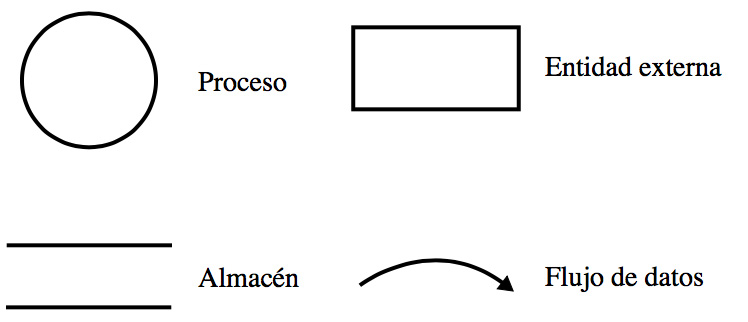
\includegraphics[width=0.5\linewidth]{Resources/elementosDFD}
  \caption{Notación estándar utilizada para representar los elementos del DFD.}
  \label{fig:elementosDFD}
\end{figure}
\begin{enumerate}
    \item \textbf{Procesos}: Representan elementos software que transforman información.
    
    \item \textbf{Entidades externas}: Representan elementos del sistema informático o de otros sistemas adyacentes que producen o consumen información transformada por el software. Los flujos de datos que comunican el sistema con las entidades externas representan las interfaces del sistema. \textbf{Sólo aparecen en el diagrama de contexto}.
    
   \item \textbf{Almacenes de datos}: Representan información almacenada que puede ser utilizada por el software. En la mayoría de los casos, utilizaremos almacenes de datos cuando los procesos intercambien información pero no estén sincronizados.
   
   \item \textbf{Flujos de datos}: Representan datos o colecciones de datos que fluyen a través del sistema. Conectan los procesos con otros procesos, con entidades externas o con almacenes de datos. Contienen información de las 3 dimensiones, aunque normalmente sólo representan las dimensiones de Función e Información.\\
   Según su \textbf{dimensión temporal}:
      \begin{enumerate}[a.]
            \item \textbf{Discretos}\textit{(Flecha con una cabeza)}: Representan movimiento de datos en un instante determinado de tiempo.
            \item \textbf{Continuos}\textit{(Flecha con con dos cabezas)}: Transmisión continua de información. 
      \end{enumerate}
\end{enumerate}

%El rabo pone bastante incapié en los niveles y utiliza una nomenclatura confusa.
\subsubsection{Niveles}
Los \textbf{DFD} permiten la representación del sistema en múltiples niveles de abstracción, de esta forma se pueden representar gráficos con un número reducido de procesos (máximo 7$\pm$2). Deberíamos usar 7-8 niveles como mucho.
\begin{enumerate}
    \item \textbf{Nivel 0}: \textbf{Diagrama de Contexto}\\
    Representa el sistema como un único proceso, el \textbf{proceso 0}. Se representan también las entidades que interactúan con el mismo, dejando claro los \textbf{límites del sistema}.
    
    %Imagen nivel 0
    \begin{figure}[h!]
  \centering
  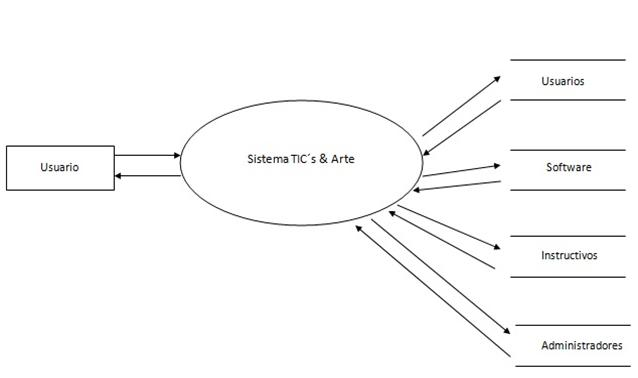
\includegraphics[width=0.45\linewidth]{Resources/niv-0}
  \caption{DFD de nivel 0 de un sistema.}
  \label{fig:dfdn0}
\end{figure}
    \item \textbf{Nivel 1}: \textbf{Diagrama 0}\\
    Denominado así porque \textit{descompone el proceso 0} en sus funciones principales. Es interesante que éstas sean \textit{independientes} y que procesen \textit{las mismos flujos} que el de nivel 0.
    %Imagen nivel 1
    \begin{figure}[h!]
  \centering
  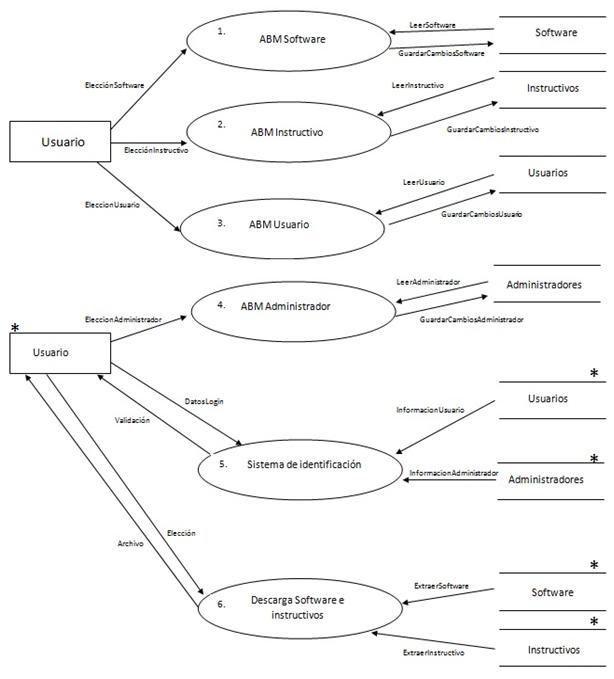
\includegraphics[width=0.45\linewidth]{Resources/nivel-1}
  \caption{DFD de nivel 1 de un sistema.}
  \label{fig:dfdn1}
\end{figure}
    \item \textbf{Niveles 2\ldots $n-1$}\\
    Continuamos descomponiendo los procesos en subprocesos, recogiendo las interfaces (flujos) de nivel superior y asignándoselas a subprocesos.
    %Imagen nivel 2
    \begin{figure}[h!]
  \centering
  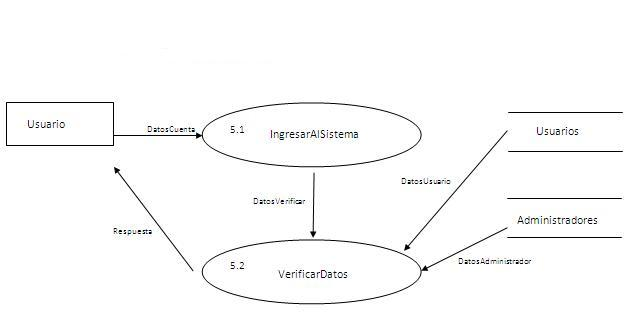
\includegraphics[width=0.45\linewidth]{Resources/nivel-2-p5}
  \caption{DFD de nivel 2 del proceso $5$ del sistema.}
  \label{fig:dfdn2}
\end{figure}
    \item \textbf{Nivel $n$}\\
    Contiene los procesos primitivos, que no podemos descomponer. Si queremos describirlo debemos utilizar técnicas de especificación de procesos.
\end{enumerate}

Los procesos en el DFD tienen un \textbf{identificador numérico}:
\begin{enumerate}
    \item Nivel 0: solo tiene un proceso: el \textbf{``0''}
    \item Nivel 1: se le asigna a cada proceso un numero secuencialmente: \textbf{\{1, 2, 3\ldots\}}
    \item Nivel 2: a cada descomposición de cada proceso se le asigna un número secuencial después de un punto. Si descomponemos el \textit{proceso 1} en 3 tendríamos los procesos: \textbf{\{1.1, 1.2, 1.3\}}
    \item Niveles 2..N: a partir de aquí vamos concatenando la versión que descomponen con el número de secuencia \textbf{sin utilizar punto}. Descomponiendo el proceso \textit{1.1} en 2 tendríamos: \textbf{\{1.11, 1.12\}}
\end{enumerate}




\subsection{Especificaciones de proceso (PSPEC)} %Vaya mierda de definición original tenía esto
El \textbf{P}rocess \textbf{Spec}ification es un documento que describe textualmente los detalles de un proceso, indicando cómo es el proceso de transformación de una información de entrada en otra de salida. 
\\
Debe ser \textbf{breve} (menor a una página) e incluir siempre \textbf{precondiciones} y \textbf{postcondiciones}.
\\
Para su elaboración, se utilizan diferentes \uline{técnicas de especificación}:

\begin{enumerate}
    \item Lenguaje natural.
    \item Diagrama de flujo.
    \item Lenguaje estructurado (Pseudocódigo).
    \item Arboles de decisión.
    \item Tablas de decisión.
\end{enumerate}
% traparaba de arbol de decisión y tabla de decisión


\subsection{Diagramas de flujo de control (DFC)}
Los \textbf{D}iagramas de \textbf{F}lujo de \textbf{C}ontrol (DFC) especifican todo el flujo de sucesos, señales y condiciones de datos del sistema.
\\
\\
%Traspa 37
Los DFC se crearon como diagramas complementarios de los DFD para suplir las carencias de los mismos:
\begin{itemize}
    \item \textbf{NO} representan el \textbf{procesamiento ni la transformación} de los flujos de control (eso se hace con las CSPECs).
    \item \textbf{NO} representan los \textbf{estados del sistema}.
\end{itemize}
Para solucionar esto el DFC añade las siguientes \uline{entidades}:
\begin{itemize}
    \item \textbf{Flujos de control}: información que determina si un proceso se activa o se detiene.
    \item \textbf{Almacenes de control}: Sirven para almacenar la información de control(estado del sistema)
    \item \textbf{Condiciones de datos}: Flujos de control generados por un proceso.
    \item \textbf{Ventanas de control}: (representadas por una barra) Indican el procesamiento de señales de control. Su comportamiento se define en las especificaciones de control (CSPEC).
    \item \textbf{Activadores de procesos} Señales de control especiales que activan o desactivan procesos tomando dos posibles valores: \texttt{ON} y \texttt{OFF}. Siguen la jerarquía de los modelos, es decir: un proceso está activo si y sólo si todos sus antecesores están activos.
    \\
    \textit{Por defecto: si no tiene activador, un proceso se considera activo si sus antecesores lo están}.
\end{itemize}

\begin{figure}[H]
  \centering
  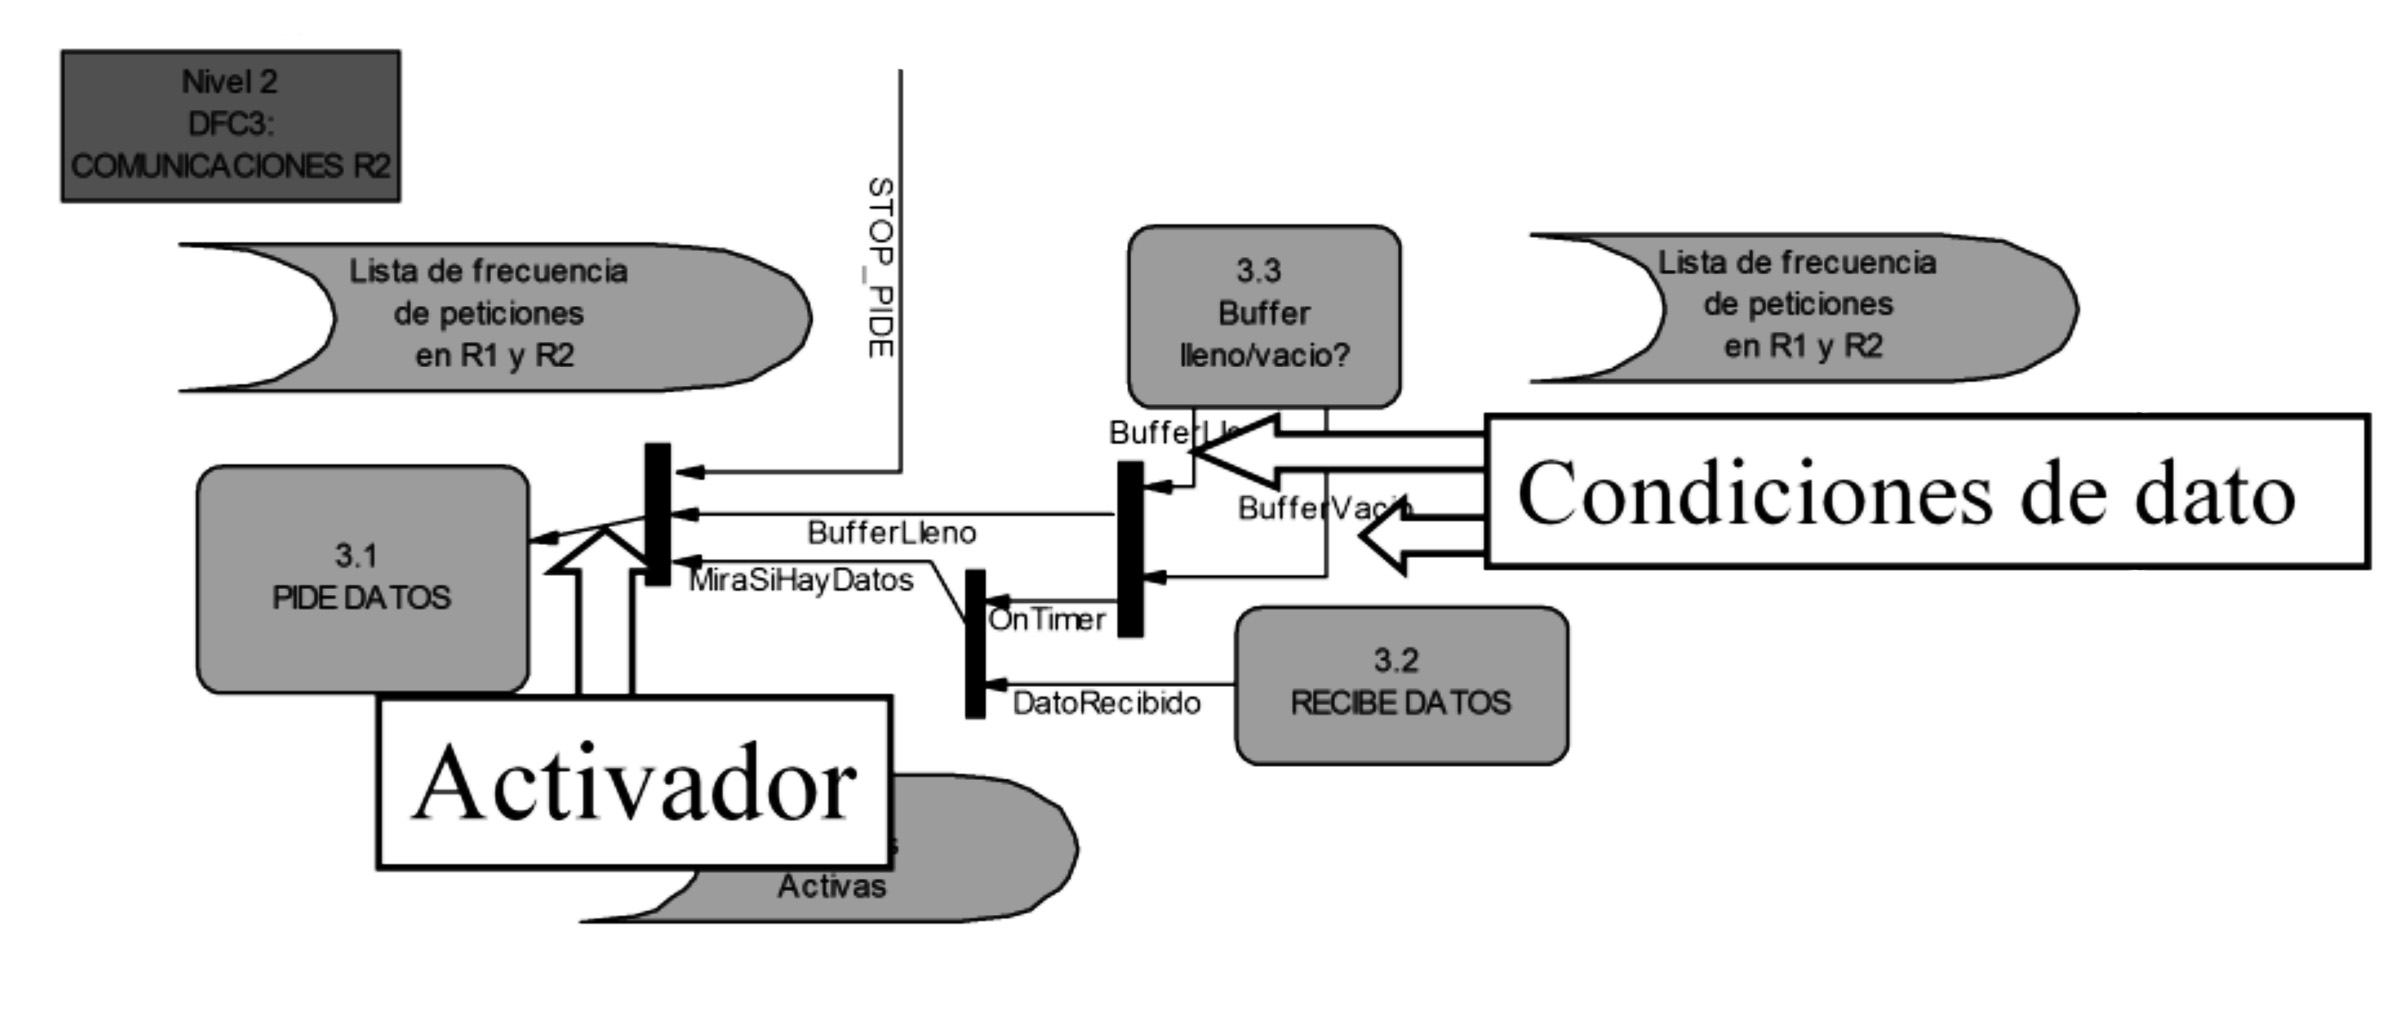
\includegraphics[width=0.9\linewidth]{Resources/ejemploDFC}
  \caption{Ejemplo de un sistema de traducción. Préstese atención a las condiciones de dato: \textit{buffer lleno/buffer vacío}, las ventanas de control (barras) y el activador.}
  \label{fig:ejemploCSPEC}
\end{figure}


\subsubsection{Construcción de un DFC}
\begin{enumerate}
    \item Se elabora una jerarquía de DFCs paralela a la de los DFDs.
    \item Cada para DFC/DFD representa los mismos procesos y las mismas entidades externas.
    \item Sólo introducimos las señales de control que no estén implícitas en el DFD.
    \item A continuación, cada DFC se desarrollará en una especificación de control (CSPEC).
\end{enumerate}


\subsection{Especificaciones de control (CSPEC)}

El \textbf{C}ontrol \textbf{SPEC}ification es un documento que \textbf{especifica de manera secuencial o combinacional el comportamiento del programa}. Indicando bajo qué condiciones se emiten las señales de control que activan los procesos.
\\ 
\\
Existirá por lo tanto una \textbf{relación 1:1 entre los CSPEC y los DFC} de la jerarquía ya que el primero determina la activación del segundo, utilizando las \textbf{ventanas de control de los DFC como interfaces}.
\\
\\
% Especificación: división entre combinacional y secuencial.
Para su elaboración, se utilizan diferentes \uline{técnicas de especificación}:
\begin{enumerate}
    \item Lenguaje estructurado (Pseudocódigo). % parseo lo de la traspa
\begin{figure}[h!]
\centering
  \begin{verbatim}
                        SI BufferVacio
                            MIENTRAS NO BufferLleno
                                ESPERA Retardo
                                OnTimer
                            FIN MIENTRAS NO
                        FIN SI
  \end{verbatim}
  \caption{Ejemplo pseudocódigo para la activación de la función \emph{OnTimer}.}
\end{figure}
    \item En sistemas combinacionales:
    \begin{itemize}
        \item Tablas de activación de procesos %parseo la de la traspa
        \begin{table}[h!]
        \centering
            \begin{tabular}{|c|c|} \cline{1-2}
             & MiraSiHayDatos \\ \hline
            3.1 & 1 \\ \hline
            3.2 & 0 \\ \hline
            3.3 & 0  \\ \hline
            \end{tabular}
            \caption{Ejemplo de tabla de activación de un proceso.}
        \end{table}

        
        %Traspa 55
        \item Tablas de decisión
            \begin{table}[h!]
                \centering
                \resizebox{0.4\textwidth}{!}{%
                    \begin{tabular}{|l|c|c|c|c|c|}
                    \hline
                    \multicolumn{6}{|c|}{\textbf{CONDICIONES}} \\ \hline
                    Condición 1 & Sí & Sí & No & No & No \\
                    Condición 2 & Sí & - & - & - & - \\
                    Condición 3 & - & Sí & - & - & - \\
                    Condición 4 & - & - & Sí & - & - \\
                     &  &  &  &  &  \\ \hline
                    \multicolumn{6}{|c|}{\textbf{ACCIONES}} \\ \hline
                    Acción 1 & X &  & X &  &  \\
                    Acción 2 &  & X &  & X & X \\\hline
                    \end{tabular}
                    }
                \caption{Ejemplo de tabla de decisiones de un proceso.}
            \end{table}
    \end{itemize}
    \item En sistemas secuenciales:
    \begin{itemize}
        \item Diagramas de estados
        \begin{figure}[h!]
          \centering
          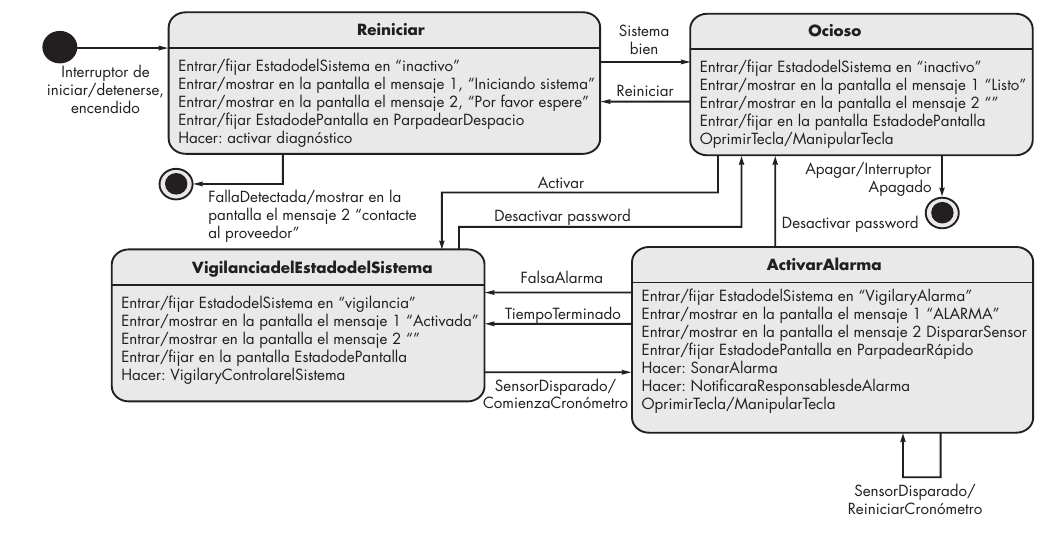
\includegraphics[width=0.9\linewidth]{Resources/estados}
          \caption{Ejemplo de un diagrama de estados.}
        \end{figure}

        \item Redes de Petri
                \begin{figure}[H]
          \centering
          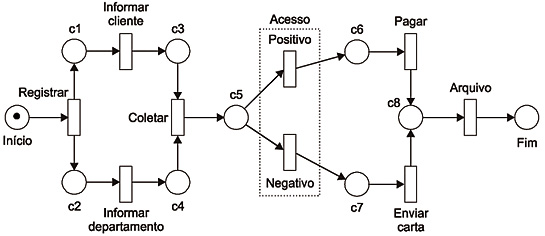
\includegraphics[width=0.9\linewidth]{Resources/redPetri}
          \caption{Proceso de generación de una reclamación modelado en redes de Petri.}
        \end{figure}
    \end{itemize}
\end{enumerate}





\subsection{Diagramas entidad--relación (DER)} % Mala definición
Los \textbf{D}iagramas \textbf{E}ntidad--\textbf{R}elación resuelven las insuficiencias que se pueden producir en la representación de los datos mediante los almacenes en los diagramas de flujo de datos (DFD), mostrando no sólo la información contenida si no las relaciones que existen entre los datos almacenados.

% no está en las traspas
% \subsection{Diccionario de datos (DD)} %No mal, quizás se pueda acortar un poquito la definición
% El diccionario de datos (DD) es un\textbf{ listado organizado de todos los elementos de datos que son pertinentes para el sistema, con definiciones precisas y rigurosas} que permiten que el usuario y el analista tengan una misma comprensión de las entradas, salidas, componentes de los almacenes y cálculos intermedios. Suele implementarse como parte de una herramienta CASE (Computer Aided Software Engineering) de análisis y diseño estructurados. El formato varía entre las distintas herramientas, pero \uline{suele contener}:
% \begin{itemize}
%     \item \textbf{ID}.%: Opcional.
%     \item \textbf{Nombre}: Único y descriptivo.%Nombre descriptivo único del elemento del almacén de datos o entidad externa.
%     \item \textbf{Alias}.%: Otros nombres.
%     \item \textbf{Dónde se usa/Cómo se usa}: Origen/Destino del flujo de datos, procesos que usan el dato y cómo lo usan.
%     \item\textbf{ Descripción del contenido}: Contenido representado según alguna notación.
%     \item \textbf{Comentarios adicionales}: Tipo de datos, valores implícitos, etc.
% \end{itemize}
% Una vez introducidos en el diccionario de datos un nombre y sus alias, se debe revisar la consistencia de las denominaciones.

% La información de dónde y cómo se usa un elemento se crea de modo automático a partir de la inspección de diagramas de control de flujo (DFC) y diagramas de flujo de datos (DFD). Mantener el diccionario de datos (DD) es extremadamente difícil para proyectos grandes, por eso las herramientas CASE son de gran ayuda. %Este párrafo creo que sobraba

\subsection{Comprobaciones a realizar sobre una especificación estructurada}
Debemos revisar si nuestra especificación cumple las siguientes propiedades.
\begin{enumerate}
    \item \textbf{Compleción}: Si los modelos son completos.
    \item \textbf{Integridad}: Si no existen contradicciones ni incoherencias entre modelos.
    \item \textbf{Exactitud}: Si los modelos cumplen los requisitos del usuario.
    \item \textbf{Calidad}: Estilo, legibilidad y facilidad de mantenimiento.
\end{enumerate}
\textit{Recomendación: checklist que compruebe a fondo que se cumplen estas propiedades}.



\subsection{Técnicas matriciales}
Las técnicas matriciales se utilizan \textbf{principalmente para ayudar a verificar la consistencia entre los componentes de distintos modelos} de un sistema.
\begin{enumerate}
    \item \textbf{Matriz entidad/función}: Visualiza las relaciones existentes entre las funciones que lleva a cabo un sistema y la información necesaria para soportarlas.\\
    Los elementos de las filas son entidades o relaciones presentes en el diagrama entidad--relación, mientras que los de las columnas pueden ser funciones de alto nivel representadas en un diagrama de flujo de datos.\\
    En cada celda se incluyen las \textbf{acciones} que puede realizar la función (\textbf{I}nsertar, \textbf{L}eer, \textbf{M}odificar y \textbf{B}orrar).
    %tabla pág 88 traparabas

 
\begin{table}[h!]
\centering
\begin{tabular}{cl|c|c|c|} \cline{3-5}
            & & \multicolumn{3}{c|}{\textbf{Funciones}}             \\ \cline{3-5}
             & & Gestionar Presupuesto & Gestionar Cliente & \ldots \\ \cline{2-5}
\parbox[t]{2mm}{\multirow{3}{*}{\rotatebox[origin=c]{90}{{\small \textbf{Entidades}}}}} & \multicolumn{1}{|c|}{Cliente}     & L           & I, M, B  &  \\ \cline{2-5}
            & \multicolumn{1}{|c|}{Presupuesto} & I, M, B  & & \\ \cline{2-5}
            & \multicolumn{1}{|c|}{\ldots} &               & & \\ \cline{2-5}    
\end{tabular}
\caption{Ejemplo de matriz entidad/función.}
\label{tab:matrizEF}
\end{table}
    
    \item \textbf{Matriz entidad/entidad}: Muestra las relaciones normales del diagrama entidad--relación.
    %tabla 89 traparaba
\begin{table}[h!]
\centering
\begin{tabular}{cl|c|c|c|} \cline{3-5}
            & & \multicolumn{3}{c|}{\textbf{Entidades}}             \\ \cline{3-5}
             & & Cliente & Presupuesto & \ldots \\ \cline{2-5}
\parbox[t]{2mm}{\multirow{3}{*}{\rotatebox[origin=c]{90}{{\small \textbf{Entidades}}}}} & \multicolumn{1}{|c|}{Cliente}     &                      & Tiene         &  \\ \cline{2-5}
            & \multicolumn{1}{|c|}{Presupuesto} & & & \\ \cline{2-5}
            & \multicolumn{1}{|c|}{\ldots} & & & \\ \cline{2-5}    
\end{tabular}
\caption{Ejemplo de matriz entidad/entidad.}
\label{tab:matrizEE}
\end{table}
    
    %mecago en dios tanto royo para definir señales de control y ahora usa eventos....
    \item \textbf{Matriz evento/entidad}: Muestra las acciones que probocan los eventos sobre las entidades: (\textbf{I}nsertar, \textbf{L}eer, \textbf{M}odificar y \textbf{B}orrar).
    %trapa raba 90
\begin{table}[h!]
\centering
\begin{tabular}{cl|c|c|c|} \cline{3-5}
            & & \multicolumn{3}{c|}{\textbf{Entidades}}             \\ \cline{3-5}
             & & Cliente & Presupuesto & \ldots \\ \cline{2-5}
\parbox[t]{2mm}{\multirow{3}{*}{\rotatebox[origin=c]{90}{{\small \textbf{Eventos}}}}} & \multicolumn{1}{|c|}{Datos del cliente}     & I, M, B           &   &  \\ \cline{2-5}
            & \multicolumn{1}{|c|}{Datos del presupuesto} & I  & I, M, B & \\ \cline{2-5}
            & \multicolumn{1}{|c|}{\ldots} &               & & \\ \cline{2-5}    
\end{tabular}
\caption{Ejemplo de matriz evento/entidad.}
\label{tab:matrizEvE}
\end{table}
\end{enumerate}

\section{Metodología del análisis estructurado}

\subsection{Fases}

\begin{enumerate}
    \item Creación del modelo de procesos: Creamos los niveles de DFDs y las PSPEC.
    \item Creación del modelo de control: para cada DFD creamos un DFC y una CSPEC.
    \item Creación del modelo de datos: si los datos son complejos utilizamos un DER.
    \item Consistencia entre modelos: podemos hacer una lista de comprobación además de tablas para comprobar la coherencia.
\end{enumerate}

\subsection{Modelos complementarios}
Fuera de estas fases tenemos dos modelos más: %no lo tengo muy claro, parece así por las traspas
\begin{enumerate}
    \item \textbf{Modelo esencial o lógico}: es un modelo de lo que el sistema debe hacer para satisfacer los requisitos del usuario. En él no figura nada acerca de cómo se va a implementar el sistema, como los ficheros de backup, o la secuenciación de proceso.
    \item \textbf{Modelo de implementación}: En él se pueden mostrar detalles técnicos:
    \begin{itemize}
        \item Elección de dispositivos y formatos E/S.
        \item Volúmenes de datos, backups, dispositivos de almacenamiento.
        \item Tiempos de respuesta.
        \item Seguridad.
    \end{itemize}
\end{enumerate}
%Tema acabado

% El recorte más grande de los apuntes XD
% \subsection{Creación del modelo de procesos} % esto se puede poner fácilmente en pasos, sería mucho más legible. Hay paja.
% Mediante el uso de diagramas de flujos de datos (DFD) y especificaciones de proceso (PSPEC) podemos modelar el ámbito de información y ámbito funcional del sistema.
% %Lo dicho, poner en pasos estudio de la documentación inicial del sistema, análisis de la información de entrada y especifiación preliminar de componentes del sistema, elaboración del DFD de contexto…
% \\
% \\
% Antes de empezar a realizar diagramas, lo primero que tenemos que hacer es estudiar toda la documentación inicial del sistema, bien sea una especificación preliminar, o el resultado de reuniones con el cliente.
% \\
% \\
% Podemos analizar gramaticalmente la información de entrada, identificando los nombres (entidades externas, flujos y almacenes de datos) y verbos (procesos o funciones) de la especificación preliminar para identificar componentes del sistema.
% \\
% \\
% Comenzaremos por hacer el diagrama de flujo de datos (DFD) de contexto, mostrando el sistema en relación con las entidades externas con las que interactúa. A continuación, lo iremos refinando en mayores niveles de detalle. Hay que aplicar los principios de acoplamiento mínimo (máxima independencia) entre procesos distintos y máxima cohesión (fuerte conexión funcional entre todo lo que está dentro de un proceso) en cada proceso. El número de procesos por DFD debería estar entre 5 y 10. Al realizar descomposiciones, hay que mantener la consistencia de nombres, numeración y flujos de datos.
% \\
% \\
% No hay que caer en detalles de implementación, el DFD tan sólo debe mostrar una visión de cómo se mueve idealmente la información entre diferentes procesos.
% Según vamos incluyendo elementos en el DFD, hay que definirlos en el diccionario de datos (DD) del proyecto.
% \\
% \\
% Seguiremos descomponiendo hasta encontrar las primitivas de proceso, que serán procesos sencillos, con máxima cohesión. Los flujos de datos que entran y salen de las primitivas constituyen las interfaces de estos procesos. Describiremos estas primitivas mediante la especificación de proceso (PSPEC), a poder ser en pseudocódigo, manteniendo la consistencia de flujos de entrada y salida con respecto a los DFD.




% \subsection{Creación del modelo de control} %Esto también se debería poner en pasos
% No todos los sistemas necesitan un modelo de control, por lo que lo primero es determinar si es necesario o no.
% \\
% \\
% Si decidimos desarrollar un modelo de control, hay que establecer una jerarquía de diagramas de flujo de control (DFC) simétrica a la de DFD, donde cada par DFD/DFC contiene los mismos procesos, almacenes de datos y entidades externas, y en la misma posición.
% \\
% \\
% Eliminaremos del DFD todos los flujos que transporten información de control, para representarlos en los DFC. Hay que tener cuidado de no caer en detalles de implementación. En aquellos casos donde el comportamiento del sistema quede reflejado implícitamente en los DFD no haremos DFC.
% \\
% \\
% A cada par DFD/DFC le corresponde una especificación de control (CSPEC). Las condiciones de datos generadas por los procesos y las señales de control provenientes del exterior del DFC entrarán en las ventanas de control, de las que saldrán los activadores de procesos y las señales de control que salgan del DFC. Hay que mantener la consistencia de flujos de control entre las ventanas de control y las CSPEC.
% \\
% \\
% La especificación de control (CSPEC) puede ser combinacional, secuencial o compuesta. Las CSPEC combinacionales se representan mediante tablas de decisión y tablas de activación de proceso. Las secuenciales, mediante diagramas de estados.



% \subsection{Creación del modelo de datos}
% En el caso de que los datos por el sistema tengan una estructura compleja, se desarrollará a mayores de los Diccionarios de Datos (DD) un modelo de datos utilizando diagramas entidad--relación (DER).


% \subsection{Consistencia entre modelos}

% Una vez realizados los distintos modelos del sistema, se deberían llevar a cabo las técnicas de consistencia entre modelos. Dado que todos los modelos que podamos realizar representan el mismo sistema, deben de ser consistentes. Existen diversas \uline{reglas para asegurar la consistencia}:

% \begin{enumerate}
%     \item \textbf{Consistencia entre el modelo de procesos y el diccionario de datos}:
%     \begin{itemize}
%         \item Cada elemento de los diagramas de flujo de datos (DFD) debe estar definido en el diccionario de datos (DD).
%         \item Cada elemento del DD tiene que estar incluido en algún flujo de datos.
%     \end{itemize}
%     \item \textbf{Consistencia entre el modelo de control y el diccionario de datos}:
%     \begin{itemize}
%         \item Cada elemento de los diagramas de flujo de control (DFC) debe estar definido en el DD.
%         \item Cada señal de control definida en el DD tiene que estar incluido en algún flujo de control.
%     \end{itemize}
%     \item \textbf{Consistencia entre el modelo de datos y el diccionario de datos}:
%     \begin{itemize}
%         \item Los objetos y almacenes de datos del diagrama entidad--relación (DER) tiene que estar definidos en el DD.
%     \end{itemize}
%     \item \textbf{Consistencia entre el modelo de procesos y el modelo de datos}:
%     \begin{itemize}
%         \item Cada almacén de los DFD debe corresponderse con un objeto o relación del DER.
%         \item Los nombres de los elementos del DER y de los almacenes de los DFD tienen que corresponderse.
%         \item Las entradas del DD deben aplicarse tanto a los almacenes de datos como a los objetos y relaciones correspondientes.
%     \end{itemize}
%     \item \textbf{Consistencia entre el modelo de procesos y el modelo de control}
%     \begin{itemize}
%         \item Cada DFC y cada especificación de control (CSPEC) están asociados a un DFD. El recíproco no es necesariamente cierto. Los procesos, entidades externas y almacenes de datos del DFD deben aparecer en el DFC correspondiente.
%         \item Cada estado del diagrama de estados (DE se asocia a un proceso o grupo de procesos del DFD, activos durante ese estado, o al sistema esperando que se produzca algún evento.
%     \end{itemize}
%     \item \textbf{Consistencia plano información--función}
%     \begin{itemize}
%         \item Todos los elementos definidos en los DER deben estar definidos en el DD.
%         \item Todos los diagramas de estructuras de datos (DED) deben aparecer en el DD.
%         \item Cada entidad y relación del DER debe ser consultada y actualizada al menos una vez por alguna función primitiva del DFD.
%     \end{itemize}
%     \item \textbf{Consistencia plano información--tiempo}
%     \begin{itemize}
%         \item Cada entidad del DED debe tener asociado un diagrama de historia de la vida de las entidades (HVE).
%         \item Por cada entidad debe existir un evento que la crea.
%         \item Las HVE de las entidades maestro deben tratar las posibles repercusiones de
% borrar esa entidad sobre las entidades detalle.
%     \end{itemize}
%     \item \textbf{Consistencia tiempo--función}
%     \begin{itemize}
%         \item Debe existir un proceso primitivo dentro de los DFC que trate cada uno de los elementos identificados en la HVE.
%     \end{itemize}
% \end{enumerate}





% \section{Modelos del sistema: esencial y de implementación} % Demasiado texto, debe ser más conciso
% El modelo esencial del sistema \textbf{es un modelo de lo que el sistema debe hacer para satisfacer los requisitos del usuario}. En él no figura nada acerca de cómo se va a implementar el sistema. Es el resultado de la fase de análisis de requisitos del sistema.
% \\\\
% A partir del modelo esencial, los diseñadores podrían decidir cómo implementar el sistema, usando la tecnología disponible.
% \\\\
% Lo normal es que el cliente también decida sobre detalles de implementación, que formarán parte del \textbf{modelo de implementación}. El desarrollo del modelo de implementación está a caballo entre análisis y diseño. No puede ser desarrollado sólo por analistas y cliente porque se necesita consejo de diseñadores e implementadores, y no puede ser realizado sólo por diseñadores e implementadores porque el usuario debe definir una gran cantidad de requisitos de implementación, que irán surgiendo en la fase de análisis.
% \\\\
% El modelo de implementación será una \textbf{versión revisada y anotada del modelo esencial, donde se especifiquen todos los detalles adicionales proporcionados por el usuario}:

% \begin{enumerate}
%     \item \textbf{La elección de los dispositivos de entrada y salida}.
%     \item \textbf{La elección de los dispositivos de almacenamiento}.
%     \item \textbf{El formato de las entradas y salidas}%: Incluye el tamaño de los datos.
%     \item \textbf{La secuencia de operaciones de entrada y salida}%: Incluye la definición de cómo el sistema va a dialogar con el usuario.
%     \item \textbf{Volumen de datos}%: De esta forma se pueden prever las necesidades de procesamiento y almacenamiento.
%     \item \textbf{Tiempo de respuesta}.
%     \item \textbf{Copias de seguridad, y descarga de datos del sistema}%: Cuándo y de qué datos es necesario realizar una copia de seguridad. Mecanismos de recuperación. <- los mecanismos de recuperación van implícitos con los de copia de seguridad
%     \item \textbf{Seguridad}%: Mecanismos para evitar accesos no autorizados
% \end{enumerate}

% \subsection{Errores típicos al hacer modelos de sistema} % Esto se refiere a un esencial-> necesitamos reordenar con el anterior párrafo, dividir en subsecciones 
% \begin{itemize}
%     \item \textbf{Secuenciar de forma arbitraria los procesos del DFD}: El único secuenciamiento de funciones que debe aparecer en los DFD es el impuesto por la dependencia de datos.
%     \item \textbf{Utilizar ficheros temporales o de backup}%: Supuesta una tecnología perfecta, no serían necesarios, por lo que no son requisitos esenciales, sino de implementación.
%     \item \textbf{Utilizar información redundante}: Más en relación con la eficiencia de la implementación que con los requisitos del modelo.
%     %La definición de redundancia es redundante. Vaya, qué redundancia más redundante parece un documento de ENSO!
% \end{itemize}
\newpage
\part{Pruebas del software}
%DONE
\section{Conceptos} %25/5/17 - 3:37AM - Las fuerzas del RABENSO intentan capturarme, pero yo resistiré. Debo finalizar LA MISIÓN. "POR CORBA", gritó un transeunte mientras el escriba Almuiña seguía con ENSO. "POR JADE", respondió Almuiña. Deja las deficiniciones como  venían en las traspas. Cuernos.

\paragraph{Verificación} Proceso de evaluación de un sistema o de uno de sus componentes para determinar si los productos de una fase dada satisfacen las condiciones impuestas al principio de dicha fase (IEEE). \textit{¿Son todas las fases \textbf{coherentes} entre sí y correctas?¿Estamos \textbf{construyendo correctamente el producto}?}

\paragraph{Validación} Proceso de evaluación del sistema o de uno de sus componentes durante o al final del desarrollo para determinar si satisface los requisitos especificados (IEEE). \textit{¿Cumple el sistema con los requisitos \textbf{del cliente}?¿Estamos construyendo \textbf{el producto correcto}?}


\paragraph{Pruebas} Actividad en la que un sistema o uno de sus componentes se ejecuta en circunstancias previamente especificadas, y cuyos resultados son observados, registrados y evaluados comprobando algún aspecto.
% era para dejarlo 100% rabo
\paragraph{Caso de prueba} Conjunto de entradas, condiciones de ejecución y resultados esperados desarrollados para un objetivo particular.\\\textit{Ejemplo: ejercitar un camino concreto de un programa o verificar el cumplimiento de un determinado requisito.} % OK entonces. Vete al 100% RABO

% Esto está puesto así en las traspas? Coincide con lo que saca el intellij?
% De dónde estás sacando que genera un fallo? T
 % de las trasparrabas. pues entonces bien.
 %
 
\paragraph{Fallo} Incapacidad de un sistema o de alguno de sus componentes para realizar las funciones requeridas dentro de los requisitos de rendimiento especificados.
 
\paragraph{Defecto} Incorrección en el software que \textbf{genera un fallo}\\
\textit{Ejemplo: un proceso, una definición de datos o un paso de procesamiento incorrectos en un programa.}
% Palabra de RABO
% todo esto del rabo, 
\paragraph{Error}
\begin{itemize}
    \item Diferencia entre un valor calculado, observado o medido y el valor verdadero, especificado o teóricamente correcto.
    \item Resultado incorrecto.
    \item Defecto.
    \item Acción humana que conduce a un resultado incorrecto.
\end{itemize}

\begin{figure}[H]
  \centering
  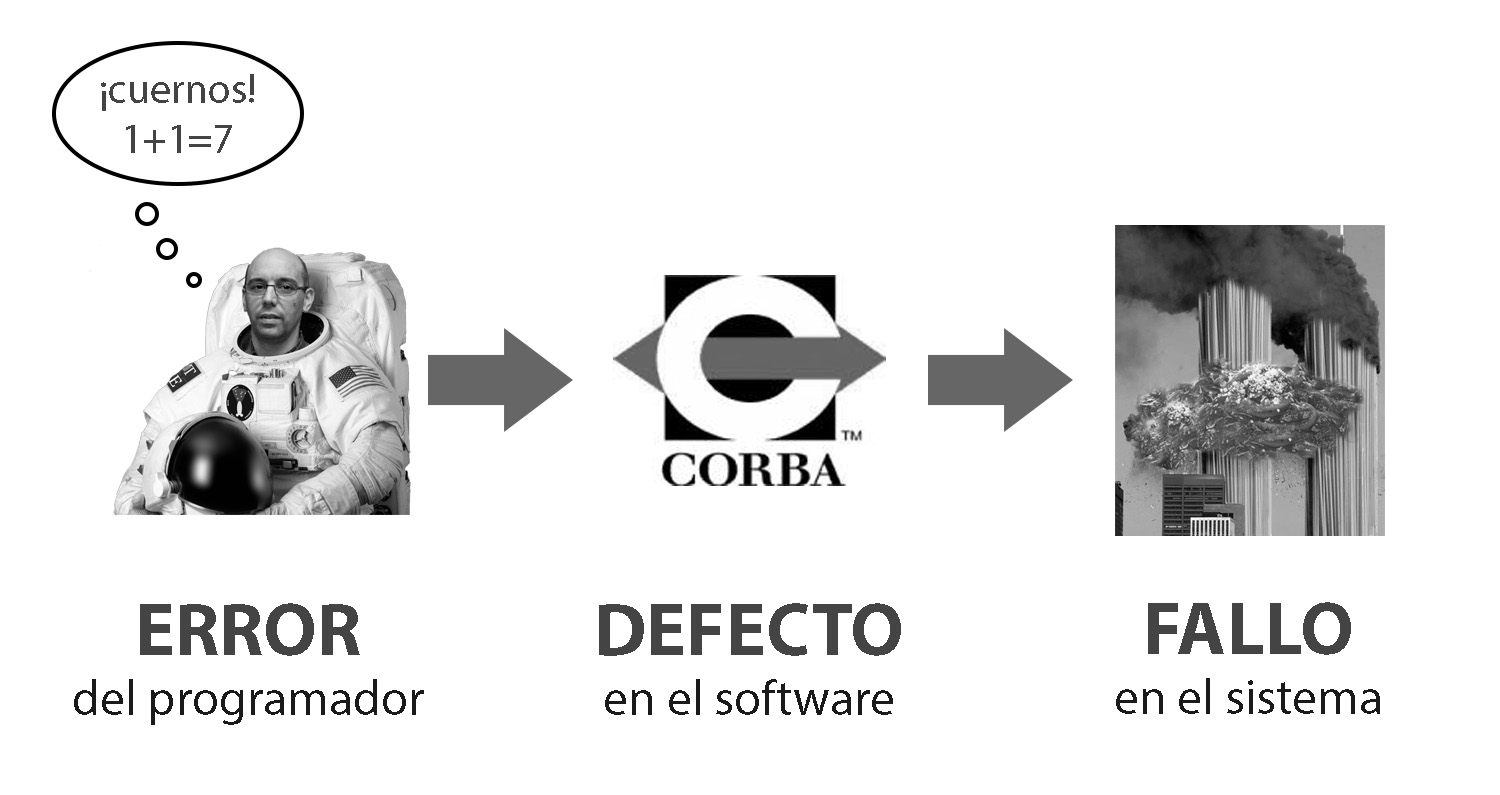
\includegraphics[width=0.8\linewidth]{Resources/cuernos}
  \caption{Recuerda: error, defecto y fallo no son lo mismo.}
  \label{fig:cuernos}
\end{figure}


\section{Filosofía de las pruebas del software}
La prueba exhaustiva del software es impracticable: \textbf{no} se pueden probar todas las posibilidades incluso en programas pequeños y sencillos. \textbf{El objetivo de las pruebas es la detección de defectos en el software en la menor cantidad de tiempo y con el menor consumo de recursos posible}.\\\\
\textbf{Descubrir un defecto constituye el éxito de la prueba}, al permitir la rectificación en el software, lo que conlleva una \textbf{mejora de la calidad}. Los defectos no siempre son el resultado de una negligencia, ya que en su aparición influyen diversos factores.

\subsection{Recomendaciones}

\begin{enumerate}
    \item \textbf{A todas las pruebas se les debería poder hacer un seguimiento hasta los requisitos del cliente}.
    \item \textbf{Las pruebas deberían planificarse mucho antes de que empiecen}: La planificación de pruebas puede comenzar tan pronto esté completo el modelo de requisitos. La definición detallada de los casos de prueba puede empezar tan pronto como el modelo de diseño se ha consolidado.
    \item \textbf{El 80\% de los errores surgen al hacer el seguimiento del 20\% de los módulos del Software (\textit{Principio de Pareto})}.
    \item \textbf{Las pruebas tendrían que hacerse de lo pequeño hacia lo grande}.
    \item \textbf{NO son posibles pruebas exhaustivas}. Sin embargo, es posible cubrir adecuadamente la lógica del programa y asegurarse de que se han aplicado todas las condiciones en el diseño a nivel de componente.
    \item \textbf{Las pruebas deberían ser realizadas por un equipo independiente del de desarrollo}: Lo ideal sería que probase el software el peor enemigo de quien lo construyó.
    \item \textbf{Cada caso de prueba debe definir el resultado de salida esperado} y compararlo con el realmente obtenido.
    \item \textbf{Se debe inspeccionar a conciencia el resultado de cada prueba} para así poder descubrir posibles síntomas de defectos.
    \item \textbf{Al generar casos de prueba se deben incluir tanto datos de entrada válidos y esperados como no válidos e inesperados}.
    \item \textbf{Las pruebas deben centrarse en probar si el software}:
    \begin{itemize}
        \item \textbf{No hace lo que debe hacer}.
        \item \textbf{Hace lo que no debe hacer}.
    \end{itemize}
    \item \textbf{Se deben evitar los casos desechables}: No documentados o diseñados sin cuidado.
    \item \textbf{No deben hacerse casos de prueba suponiendo que no hay defectos en los programas}.
    \item \textbf{Las pruebas son una tarea tanto o más creativa que el desarrollo de software}.
\end{enumerate}




% Esto no es rabo canónico
% \section{El proceso de prueba}

% \begin{enumerate}
%     \item \textbf{Generación de un plan} de pruebas. En base a la documentación sobre el proyecto y sobre el software a probar.
%     \item \textbf{Diseño} de pruebas específicas. A partir del plan.
%     \item \textbf{Ejecución} de las pruebas sobre el software.
%     \item \textbf{Evaluación} de los datos de salida. A partir de ella se pueden realizar 2 actividades:
%     \begin{itemize}
%         \item \textbf{Depuración}: Puede corregir o no los defectos; si no consigue localizarlos, puede ser necesario realizar pruebas adicionales para obtener más información. Si se corrige un defecto, se debe volver a probar el software.
%         \item \textbf{Análisis de errores}: Puede servir para realizar predicciones de la fiabilidad del software y para detectar las causas más habituales de error.
%     \end{itemize}
% \end{enumerate}

\section{Jerarquía de de la documentación de diseño de pruebas}
%Diapositiva 9 p(ongo iimamgaenge)si

De acuerdo con el \textbf{estándar IEEE 829} Se generarán la siguiente documentación:
\begin{enumerate}
    \item \textbf{Plan de pruebas}: Establece las líneas generales del plan, especificando qué elementos y funcionalidades se van a probar, personal responsable, metodologías seguidas\ldots 
    % Level Test Plan (LTP): For each LTP the scope, approach, resources, and schedule of the testing activities for its specified level of testing need to be described. The items being tested, the features to be tested, the testing tasks to be performed, the personnel responsible for each task, and the associated risk(s) need to be identified.
    \item \textbf{Especificación del diseño de pruebas}: Detalla los casos de prueba y los resultados esperados así como los criterios de paso de prueba. % Level Test Design (LTD): Detailing test cases and the expected results as well as test pass criteria.

    \item \textbf{Especificación de los casos de prueba}: Definen los datos de prueba (entradas y salidas) usados en la ejecución de los casos de prueba. % Level Test Case (LTC): Specifying the test data for use in running the test cases identified in the Level Test Design.
    
    
    \item \textbf{Especificación de procedimiento de las pruebas}: Detalla cómo se ejecutará cada uno de los casos de prueba y los pasos necesarios a seguir.
    
    \item Documentos de ejecución (\textbf{para Taboada el IEEE 1008})\footnote{Rabenso divide la documentación de pruebas en dos estándares: el IEEE 829 y el 1008. De acuerdo, con el IEEE 829--2008, esto no sería necesario pues éste estándar es más completo e incluye todas las fases.}:
    \begin{itemize}
        \item \textbf{Histórico de pruebas}: provee cronológicamente detalles relevante sobre la ejecución de las pruebas informando de cuáles fueron ejecutadas, quién las ejecutó, en qué orden y si pasaron o fallaron la prueba.
        % To provide a chronological record of relevant details about the execution of tests, e.g. recording which tests cases were run, who ran them, in what order, and whether each test passed or failed.
        \item \textbf{Informe de incidentes}: informa de cualquier problema, incidente o defecto que ocurra durante la ejecución de las pruebas que requiera investigación.
    \end{itemize}
    \item \textbf{Informe resumen de pruebas}: sumario de los resultados y evaluaciones y recomendaciones basadas en éstos. Realizado tras la finalización de la ejecución de las pruebas.
        % Level Test Report (LTR): To summarize the results of the designated testing activities and to provide evaluations and recommendations based on the results after test execution has finished for the specific test level
\end{enumerate}
\begin{figure}[H]
  \centering
  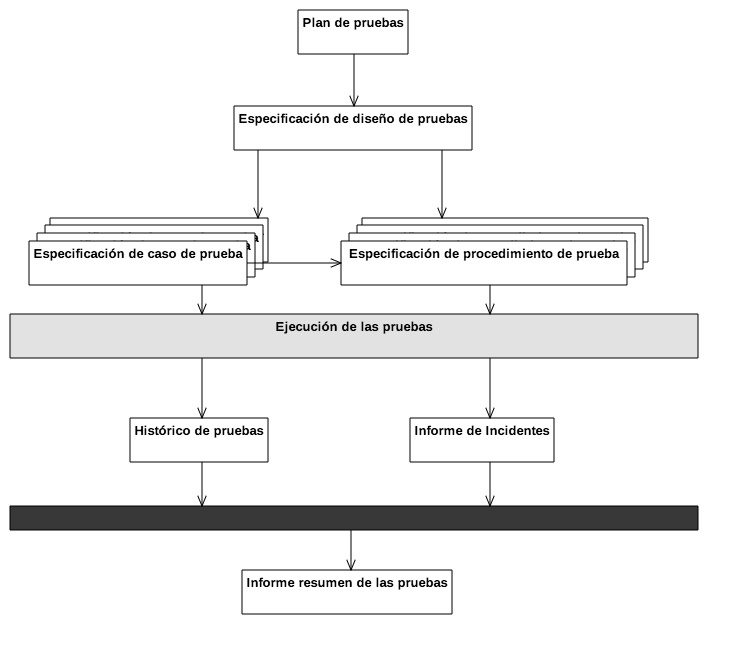
\includegraphics[width=0.6\linewidth]{Resources/IEEE829}
  \caption{El estándar IEEE 829--2008 para la realización de pruebas del software diferencia tres fases: especificación del plan de pruebas, ejecución, y elaboración de informes.}
  \label{fig:IEEE829}
\end{figure}

\section{Técnicas de diseño de casos de prueba}
Dos enfoques principales:
\begin{enumerate}
    \item \textbf{Caja negra: sólo necesitamos conocer la interfaz del elemento probado, probamos si las salidas se corresponden con la entrada. Enfoque funcional}
    \item \textbf{Caja blanca: conocemos las interioridades del sistema, probaremos que los componentes internos funcionan bien y encajan correctamente. Enfoque estructural}
\end{enumerate}
\subsection{Pruebas de caja negra (funcionales)} 

Dado que no es posible probar todo, esta sección recoge varias estrategias de creación de pruebas de caja negra que aumentan las posibilidades de descubrir errores:

\begin{enumerate}
    \item \textbf{Clases de equivalencia}: Identificamos los rangos en las restricciones de entrada o los tipos de entrada que producen un tipo de salida. Debemos \textbf{probar un valor dentro de cada rango o tipo}.
    \item \textbf{\textbf{A}nálisis de \textbf{V}alores \textbf{L}ímite (\textbf{AVL})}: Consiste en probar los errores que están en los límites de las clases de equivalencia.
    \item \textbf{Conjetura de errores}: Se prueban errores que los programadores cometen con frecuencia, bien partiendo de una lista de errores frecuentes o de la intuición del creador de la prueba.
    \item \textbf{Pruebas aleatorias}: Generamos permutaciones aleatorias de los valores de entrada y comprobamos si la salida es correcta.
\end{enumerate}

% no sale en las traspas y no me suena de clase
% \subsubsection{Métodos basados en grafos}

% La prueba del software empieza creando un grafo (colección de nodos que representan objetos, enlaces que representan relaciones entre objetos, pesos de nodos que describen las propiedades de un nodo, y pesos de enlaces que describen las características de un enlace).
% \\\\
% \uline{Métodos de prueba de comportamiento que pueden hacer uso de grafos}:
% \begin{enumerate}
%     \item \textbf{Modelado del flujo de transacción}: Los nodos representan los pasos de alguna transacción y los enlaces representan conexiones lógicas entre los pasos.
%     \item \textbf{Modelado de estado finito}: Los nodos son estados del software observables por el usuario y los enlaces son las transiciones que ocurren para moverse de un estado a otro.
%     \item \textbf{Modelado del flujo de datos}: Los nodos son objetos de datos y los enlaces son las transformaciones que ocurren para convertir un objeto de datos en otro.
% \end{enumerate}
% Cada relación en el grafo es estudiada separadamente, de manera que se puedan obtener casos de prueba. Se estudia la transitividad de relaciones secuenciales para determinar cómo se propaga el impacto de las relaciones a través de los objetos definidos en el grafo. La simetría de una relación también es importante para el diseño de casos de prueba; si un enlace es bidireccional, debería probarse esta característica. Todos los nodos del grafo deberían ser reflexivos, es decir, tener una relación que los devuelva a ellos mismos.




\subsection{Pruebas de caja blanca (estructurales)} 
El diseño de casos tiene que basarse en la \textbf{elección de caminos importantes que ofrezcan una seguridad aceptable de descubrir un defecto}, y para ello se utilizan los criterios de cobertura lógica. No requieren el uso de representaciones gráficas, pero se suelen utilizar grafos de flujo.

\begin{figure}[H]
  \centering
  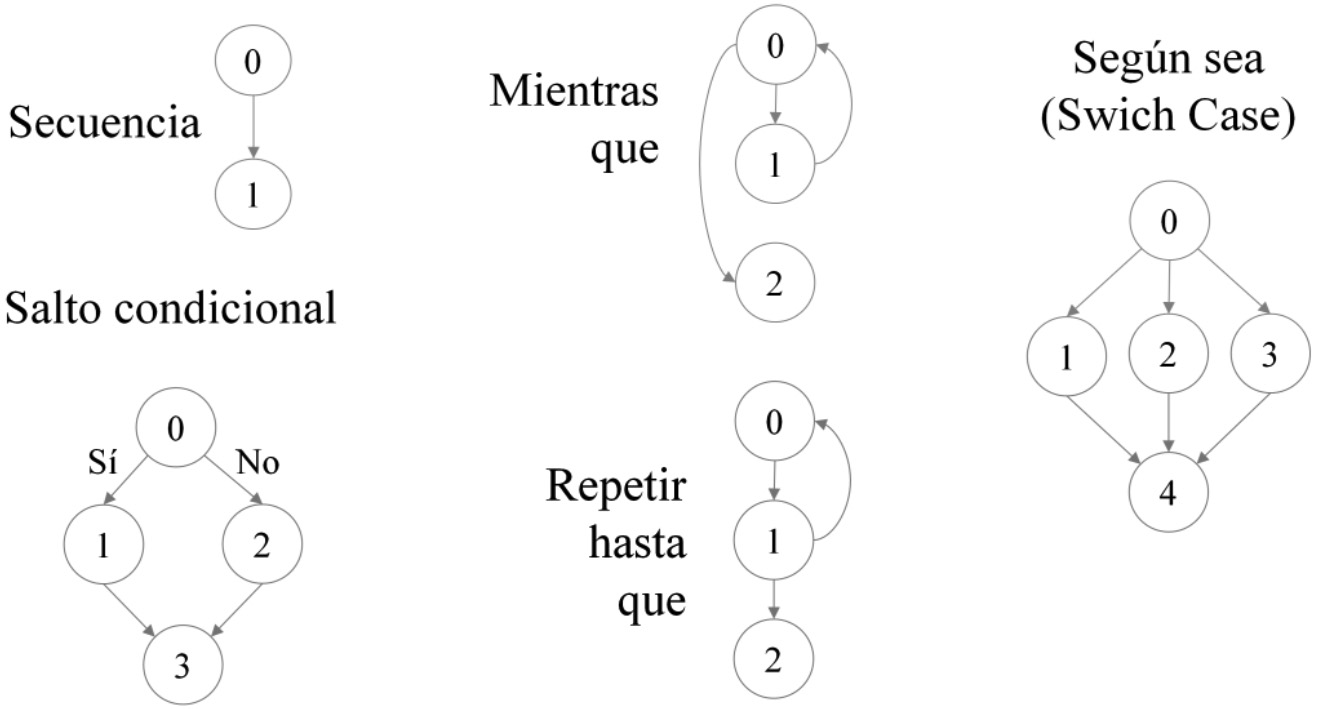
\includegraphics[width=0.6\linewidth]{Resources/ejemplosBasicosGrafos}
  \caption{Grafos básicos.}
  \label{fig:ejemplobasicografos}
\end{figure}

\subsubsection{Criterios de cobertura lógica}

\begin{enumerate}
    \item \textbf{Cobertura de sentencias}: Cada sentencia o instrucción del programa se ejecuta al menos una vez.
    
    \item \textbf{Cobertura de decisiones}: Cada decisión tiene, al menos una vez, un resultado verdadero y uno falso. En general, la cobertura de decisiones asegura la cobertura de sentencia.
    
    \item \textbf{Cobertura de condiciones}: Cada condición de cada decisión adopta, al menos una vez, un resultado verdadero y otro falso. No garantiza la cobertura de decisiones.
    
    \item \textbf{Criterio de decisión/condición}: Exigir el criterio de cobertura de condiciones obligando a que se cumpla también el criterio de decisiones.
    
    \item \textbf{Criterio de condición múltiple}: Descompone cada decisión múltiple en una secuencia de decisiones unicondicionales\footnote{una decisión es un conjunto de condiciones, por ejemplo en 
    \texttt{a != null \&\& a.leng > 3} es una decisión que se descompone en las condiciones \texttt{a != null} y \texttt{a.leng > 3}} y luego se exige que cada combinación posible de resultados de cada condición se ejecute al menos una vez. %WTF condiciones unicondicionales, eso hay que revisarlo…
    
    \item \textbf{Cobertura de caminos}: Cada uno de los posibles caminos del grafo de caminos  se ejecuta al menos una vez. Según las veces que recorramos el bucle tenemos diferentes tipos:
    \begin{itemize}
        \item Sin entrar en su interior.
        \item Ejecutándolo una vez.
        \item Ejecutándolo dos veces.
        \item Ejecutándolo n veces.
    \end{itemize}
\end{enumerate}



\subsubsection{Prueba de bucles}
La prueba de bucles es la \textbf{técnica de prueba de caja blanca que se centra exclusivamente en la validez de las construcciones de bucles}. Se pueden definir 4 clases de bucles:
\begin{enumerate}
    \item \textbf{Bucles simples}: Se les debe aplicar el siguiente conjunto de pruebas:
    \begin{itemize}
        \item Pasarlo por alto.
        \item Pasar una vez por el bucle.
        \item Pasar 2 veces por el bucle.
        \item Hacer $m$ pasos con $m < n$ tal que $n$ es el mayor número de pasos permitidos por el bucle.
        \item Hacer $n-1$ y $n+1$ pasos
    \end{itemize}
    \item \textbf{Bucles anidados}:
    \begin{itemize}
        \item Comenzar por el bucle más interior con los otros en sus valores mínimos.
        \item Llevar a cabo la prueba de bucle simple al más interior.
        \item Progresar hacia fuera, manteniendo el resto de bucles externos en sus valores mínimos y los demás bucles anidados en sus valores típicos.
        \item Continuar hasta probar todos los bucles.
    \end{itemize}
    \item \textbf{Bucles concatenados}: Se pueden probar mediante el enfoque para bucles simples siempre que cada bucle sea independiente del resto. Si son dependientes se usa la técnica para bucles anidados.
    \item \textbf{Bucles no estructurados}: Se deben rediseñar para que se ajusten a las construcciones de la programación estructurada.
\end{enumerate}



\subsubsection{Utilización de la complejidad ciclomática de McCabe}
La \textbf{métrica de McCabe es un indicador del número de caminos independientes que existen en un grafo}.\\
El propio McCabe definió como un buen criterio de prueba la consecución de la ejecución de un conjunto de caminos independientes, lo que implica probar un número de caminos igual al de la métrica. La métrica de McCabe \textbf{asegura la cobertura de sentencia y sería equivalente a la cobertura de decisiones}.
\\\\
\textbf{Un camino es independiente de otros si incorpora un arco que los demás no incluyen}. La métrica de McCabe coincide con el número máximo de caminos independientes que puede haber en un grafo. \uline{Formas de calcular la complejidad ciclomática de McCabe}:
\begin{enumerate}
    \item $V (G) = a-n+2$, siendo $a$ el número de arcos y $n$, el de nodos.
    \item $V (G) = r$, siendo $r$ el número de regiones cerradas del grafo. Si el programa tiene un nodo de inicio y otro de final, la región externa se suma como región cerrada.
    \item $V (G) = c+1$, siendo $c$ el número de nodos de condición.
\end{enumerate}

Para ayudar a la elección de los caminos de prueba, McCabe propone el \textbf{método del camino básico, consistente en realizar variaciones sobre la elección de un primer camino de prueba típico}. A partir de estos caminos, se analiza el código para conocer los datos de entrada necesarios, y se consulta la especificación para conocer la salida teóricamente correcta.\\\\
\textbf{Puede suceder que las condiciones necesarias para que la ejecución pase por un determinado camino no se puedan satisfacer de ninguna manera (camino imposible}), en cuyo caso deberemos sustituir ese camino por otro posible que permita satisfacer igualmente el criterio de prueba de McCabe.
\\\\
$V (G)$ marca un límite mínimo de número de casos de prueba para un programa. Si $V (G)$ es mayor que 10, la probabilidad de encontrar defectos aumenta, salvo que sea debido a sentencias \textit{switch case} o similares. En estos casos se debe replantear el diseño modular obtenido.



\section{Enfoque práctico recomendado para el diseño de casos}

\begin{enumerate}
    \item \textbf{Si la especificación contiene combinaciones de condiciones de entrada, comenzar formando sus grafos causa--efecto}.
    \item \textbf{Usar el análisis de valores límite (AVL) para añadir casos de prueba}: Elegir límites para dar valores a las causas en los casos generados, asumiendo que cada caso es una clase de equivalencia.
    \item \textbf{Identificar las clases válidas y no válidas de equivalencia para la entrada y la salida y añadir los casos no incluidos anteriormente}.
    \item \textbf{Utilizar conjetura de errores para añadir nuevos casos referidos a valores especiales}.
    \item \textbf{Ejecutar los casos generados hasta el momento y analizar la cobertura obtenida}.
    \item \textbf{Examinar la lógica del programa para añadir los casos precisos para cubrir el criterio de cobertura elegido} si no ha sido satisfecho en el punto anterior.
\end{enumerate}

Esto es \textbf{aplicable tanto a pruebas de caja blanca como de caja negra} ya que:
\begin{itemize}
    \item Los errores lógicos y las suposiciones incorrectas son inversamente proporcionales a la probabilidad de que se ejecute un camino del programa.
    \item Se suele creer que un determinado camino tiene pocas probabilidades de ejecutarse cuando se ejecuta regularmente.
    \item Los errores tipográficos son aleatorios.
    \item La probabilidad e importancia de un trozo de código se suele calcular de modo subjetivo.
    \item Una prueba exhaustiva de caja blanca no asegura la detección de los defectos de su diseño.
\end{itemize}



\subsection{Depuración}
La depuración es el \textbf{proceso de localizar, analizar y corregir los defectos que se sospecha que contiene el software}. Suele ser la consecuencia de una prueba con éxito. Tras corregir el defecto, se efectuarán nuevas pruebas que comprueben si se ha eliminado dicho problema.

\subsection{Análisis de errores a análisis casual}
El análisis causal \textbf{proporciona información sobre la naturaleza de los defectos para que así el personal pueda prevenirlos en el futuro}. Se recoge la siguiente información:
\begin{itemize}
    \item Cuándo se cometió.
    \item Quién lo cometió.
    \item Qué se hizo mal.
    \item Cómo se podría haber prevenido.
    \item Por qué no se detectó antes.
    \item Cómo se podría haber detectado antes.
    \item Cómo se encontró el error.
\end{itemize}

No debe usarse para evaluar al personal.

\section{Estrategia de aplicación de las pruebas}
%gráfico traspa 87
\begin{enumerate} % 
    \item \textbf{Prueba de unidad}: Se centra en ejercitar la lógica del módulo y los distintos aspectos de la especificación de las funciones que debe realizar el módulo.
    \item \textbf{Prueba de integración}: Debe tener en cuenta los mecanismos de agrupación de módulos fijados en la estructura del programa, así como las interfaces entre componentes.
    %\item \textbf{Prueba de validación}: Debe comprobar si existen desajustes entre el software y los requisitos fijados para su funcionamiento en la especificación de requisitos software (ERS). %Esta prueba no está en las trasparrabas. Por lo tanto, no existe
    \item \textbf{Prueba del sistema}: Debe comprobar el cumplimiento de los objetivos indicados para el sistema.
    \item \textbf{Prueba de aceptación}: El usuario verifica en su entorno si acepta el producto.
\end{enumerate}
\begin{figure}[H]
  \centering
  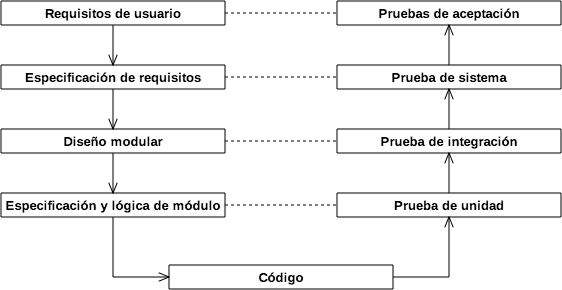
\includegraphics[width=0.7\linewidth]{Resources/enfoquePruebas}
  \caption{Las diferentes estrategias de prueba y su relación con las otras fases del construcción del software}
  \label{fig:estrategiasPruebas}
\end{figure}


\newpage
\section{Pruebas en desarrollos orientados a objetos}
\subsection{Desde el punto de vista de diseño de casos de pruebas}
\begin{itemize}
    \item \textbf{Las técnicas de caja negra}: Totalmente válidas.
    \begin{itemize}
        \item Análisis de valores límite, tratamiento de combinaciones de entrada y conjetura de errores.
        \item Debemos diseñar las pruebas basándonos en datos y eventos de los escenarios de los casos de uso y en flujos alternativos, tratamientos de error y excepciones.
    \end{itemize}
    \item \textbf{Las técnicas de caja blanca}: Disminuyen sus posibilidades de aplicación. Quedan confinadas a las instrucciones de cada método de cada clase.
\end{itemize}

\subsection{Desde el punto de vista del nivel}
Los cambios más radicales aparecen en las pruebas de integración, cuando nos fijamos en la interacción entre objetos de distintas clases. El enfoque habitual consiste en ir probando hilos de clases que colaboran para una función o servicio del sistema.

\subsection{Cuestiones a tener en cuenta}
Ciertas cuestiones a tener en cuenta a la hora de probar software orientado a objetos son:
\begin{itemize}
\item \textbf{Herencia}: probar un método de la clase padre no garantiza su funcionamiento en clases hijas.
\item \textbf{Polimorfismo}: un único método puede tener implementaciones diferentes en función de la clase en la que se use.
    \item Es conveniente recordar que la propia programación o diseño orientado a objetos hace menos probables ciertos tipos de error, más probables otros, y provoca la aparición de nuevos tipos de defectos. %Pues OC, mejor redactado.
\end{itemize}

\newpage
\section{Ejemplo práctico de cálculo de la complejidad ciclomática de un método}
Dado el método  \texttt{public String porcentajeVentasMes();} tal que: 
\begin{verbatim}
public String porcentajeVentasMes() {
	    [...]
	//recopilamos precios por dia
    for(int i = 0 ; i < ventas.size() ; i++ ){
        Venta v=ventas.get(i);
        Calendar cal = Calendar.getInstance();
        targetCalendar.setTime(cFecha.toDate(v.getFecha()));
        precios[cal.get(Calendar.DAY_OF_MONTH)]+=v.getPrecioUnidad();
        total+=v.getPrecioUnidad();
    }

    //calcula los porcentajes
    for(int i = 0 ; i < columnas; i++ ){
        if(precios[i]>0){
        	porcentajeVentas+="Día "+(i+1)+": "+
        	+ BigDecimal.valueOf(precios[i]/total*100)
        		        .setScale(2, RoundingMode.HALF_UP)
        		        .doubleValue()+"%\n";
        }
        return porcentajeVentas;
    }
}   
\end{verbatim}

\begin{figure}[H]
  \centering
  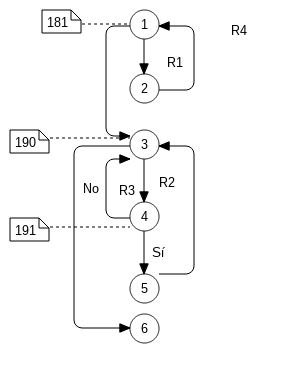
\includegraphics[width=0.4\linewidth]{Resources/porcentajeVentasMes}
  \caption{Grafo de flujo del método.}
  \label{fig:joder}
\end{figure}
\newpage
\paragraph{Caminos básicos obtenidos}
    \begin{enumerate}
        \item 1-3-6
        \item 1-\underline{2}-1-3-6
        \item 1-3-\underline{4}-3-6
        \item 1-2-3-4-\underline{5}-3-6
    \end{enumerate}

\paragraph{Caminos independientes:} 3
    \begin{enumerate}
        \item 1-(3-4)\textsuperscript{x31}-3-6
            \begin{itemize}
                \item No puede existir en el sistema ninguna venta realizada en el mes actual.
                \item La variable \texttt{columnas} sólo podrá poseer los valores 28, 29, 30 ó 31, dependiendo del mes en el que es ejecutada la función. Es por esto que no se puede llevar a cabo ningún camino que contenga 1-3-6.
            \end{itemize}
        \item 1-2-(3-4)\textsuperscript{x31}-3-6
            \begin{itemize}
                \item Para seguir este camino independiente, deberá existir  una venta realizada en el mes actual, o más si se desea repetir más veces el segmento 1-2.
                \item Ningún artículo podrá tener un precio superior a 0 para poder seguir este camino estrictamente.
            \end{itemize}
        \item 1-(3-4)\textsuperscript{x31}-3-6
            \begin{itemize}
                \item Equivalente al camino 1.
            \end{itemize}
        \item 1-2-(3-(4\textbar{}\textbar{}(4-5)))\textsuperscript{x31}-3-6
            \begin{itemize}
                \item Para seguir este camino independiente, deberá existir  una venta realizada en el mes actual con un precio por unidad superior a 0 o más si se desea repetir más veces el segmento 3-4-5.
            \end{itemize}
    \end{enumerate}
\newpage

\part{Preguntas de examen}

\section{Resolución de preguntas cortas}
Las preguntas cortas consistirán en refutar sentencias falsas en base a vuestros conocimientos de la asignatura. En ningún caso se tratará de contar todo lo que sabéis sobre el punto en cuestión de que trate la frase sino sólo de rebatir la falacia con argumentos objetivos y precisos. Las respuestas de más de 10 líneas no serán evaluadas, ya que entiendo que siempre debería poder responderse como máximo en 5 o 6.

\subsubsection*{1. Las normas de procesos para la construcción del software sólo describen procesos que tienen por objetivo el desarrollo de código ejecutable.}
\textit{Todas las normas vistas describen procesos incluidos en todo el ciclo de vida del software. Las normas ISO 12207 e ISO/IEC 15504 incluyen entre sus procesos principales los de adquisición y suministro (gestionan la compra-venta); también incluyen los procesos de soporte (describen tareas de apoyo, no de construcción) y los de la organización, que ni siquiera tienen que ver con el desarrollo de un proyecto software concreto. De hecho la codificación se tratar sólo como una actividad del proceso de desarrollo en estas normas.
\\
También se puede hacer el mismo razonamiento con la norma IEEE 1074 que nos proporciona 4 secciones lógicas de las que sólo una tiene que ver con el desarrollo. Las otras tres tienen que ver con la selección del ciclo de vida, la gestión del proyecto y los procesos integrales, vinculados a asegurar la terminación y calidad de los procesos.}

\subsubsection*{2. Sólo el SEI americano ha mostrado interés en la generación de normas para la Ingeniería del Software debido a su carácter académico.}
\textit{Como se ha discutido indirectamente en la pregunta anterior, las normas del IEEE y la ISO/IEC acreditan la preocupación de otras instituciones, independientes del SEI, por la formalización de estas normas. Además estos estándares, como se demuestra en la explicación del CMMI, están orientados a su aplicación en las empresas a las que deben proporcionar un marco válido que evite el desarrollo ad hoc de aplicaciones.}

\subsubsection*{3. Pasar del modelo en cascada al modelo incremental no solucionó ningún problema de ingeniería pero permitió ganar más dinero a los programadores.}
\textit{El salto al modelo incremental evita la concepción monolítica del software que da el modelo en cascada. Propone un modelo iterativo que permite la evolución en sus requisitos, la mejora de la comunicación con el cliente y posibilita reducir el coste de los errores.}

\subsubsection*{4. Ante un problema ya resuelto el planteamiento siempre debe ser reprogramar otra solución pues seguro que será más eficiente.}
\textit{Si el problema está resuelto implica que el software ya existe. La conclusión de los análisis de coste realizados en prácticas y la discusión sobre el reuso hecha en clase, es que será más barato (y por tanto eficiente) comprarlo que reconstruirlo. Sólo debemos plantearnos construir cuando la funcionalidad que necesitamos no está recogida por el software disponible o se precisa una modificación significativa para adaptarlo. Evidentemente no se considera que la funcionalidad esté en la aplicación si ésta no la realiza con la calidad esperada.}

\subsubsection*{5. Los únicos riesgos posibles de un proyecto son económicos y técnicos}
\textit{Si bien estos riesgos importantes, existen otro tipo de riesgos que pueden resultar cruciales a la hora de desarrollar un proyecto. Es el caso de los riesgos geopolíticos, desastres naturales, realizar un mal análisis de requisitos, realizar una mala planificación, o el espionaje industrial.}

\subsubsection*{6. La única cualidad importante del analista es ser persuasivo para convencer al cliente de que el software que le desarrollamos era el que necesitaba.}
\textit{En tanto que la persuasión es cualidad importante y forma parte de una de las muchas dotes comunicativas que debe tener un analista, no es suficiente.
\\
Un analista debe ser capaz de comunicar y de extraer información de los clientes.\\
Además, valiéndose de sus conocimientos técnicos y experiencia en el campo de la ingeniería del software, ser capaz de traducir ideas vagas de necesidades de software en un conjunto concreto de funciones y restricciones.
}

\subsubsection*{7. La especificación es un documento escrito en lenguaje natural que será tanto mejor cuanto más largo y enrevesado sea.}
\textit{Una especificación es un documento descriptivo, que debe reflejar de forma clara y sencilla el aspecto del software que esté tratando.\\
Por lo tanto, se deberá evitar el uso del lenguaje natural (puesto que puede resultar vago y ambiguo) y, en su defecto, hacer uso de modelos, diagramas y herramientas que reflejen objetivamente el software.\\
Por otro lado, los documentos generados deben estar estructurados en particiones, permitiéndonos detectar cualquier redundancia y facilitando su modificación y lectura.
}

\subsubsection*{8. Un buen modelo es aquel que, sin ayuda de otros, representa todos los aspectos de un sistema.}
\textit{Debido a la complejidad de los sistemas informáticos, no es posible elaborar un modelo comprensible para un ingeniero que represente todos los aspectos de un sistema de forma clara y concisa.
\\
Es por ello que debemos optar por una estrategia fragmentada, representando el sistema mediante múltiples modelos que colaboren entre sí y nos permitan reflejar con precisión cada uno de los aspectos del sistema.
}

\subsubsection*{9. Cada DFD y DFC tienen los mismos procesos y almacenes pero jamás se relacionan ya que uno representa la función y el otro el comportamiento.} %No me gusta la argumentación que efrén propone para esta respuesta. recomendaría su revisión y reescritura.
\textit{Los DFD y DFC están íntimamente relacionados pues el DFC es la representación del flujo de control de los procesos definidos en el DFD que representa. Los procesos y almacenes sí son los mismos en los dos diagramas. El DFC representa el comportamiento de los procesos definidos en el DFD.
}

\subsubsection*{10. Los casos de prueba son las entradas necesarias al sistema para que se ejecute un camino de prueba que garantice la cobertura de sentencia.}

\begin{enumerate}
    \item \textit{La motivación de hacer una prueba es encontrar un fallo, a partir de ahí hay múltiples  metodologías para realizar una prueba, existen pruebas de caja negra y blanca y dentro de las de caja blanca estaría un tipo cuyo objetivo es la cobertura de sentencia.}
    \item \textit{ De acuerdo con el IEEE 829, en la especificación de un caso de prueba se definen tanto las entradas como las salidas (datos de prueba) usados en la ejecución de los casos.}
\end{enumerate}

% \\
% Por otra parte, la cobertura de sentencia no es la única posible y de acuerdo con nuestras necesidades puede ser necesario cubrir otro tipo de coberturas como por ejemplo las de decisiones, condiciones o de caminos.
% }



\subsubsection*{11. ¿Cuáles son los puntos de vista desde los que podemos modelar el software? Sitúa en una tabla que tenga los puntos de vista tanto en las filas como en las columnas, y las metodologías o técnicas que conozcas para modelar}
\begin{table}[ht]
\centering
\resizebox{\textwidth}{!}{
    \begin{tabular}{c|l|l|l|} \cline{2-4}
        &   \multicolumn{1}{c|}{\textbf{Información}} &   \multicolumn{1}{c}{\textbf{Función}} &   \multicolumn{1}{|c|}{\textbf{Tiempo}}   \\ \hline
        
        \multicolumn{1}{|c|}{\multirow{4}{*}{\textbf{Información}}} &   D. entidad--relación        &   &   \\
        \multicolumn{1}{|c|}{}    &   D. de estructura de datos   &   &   \\
        \multicolumn{1}{|c|}{}    &   Matriz entidad/entidad      &   &   \\
        \multicolumn{1}{|c|}{}    &   Diagramas de clases         &   &   \\ \hline
        
        \multicolumn{1}{|c|}{\multirow{7}{*}{\textbf{Función}}}    & D. de flujo de datos  &   D. de flujo de datos   &    \\
        \multicolumn{1}{|c|}{}    &   Matriz función/entidad  & D. de casos de uso    &   \\
        \multicolumn{1}{|c|}{}    &   Diagrama de clases  &   D.de estructura de datos    &   \\
        \multicolumn{1}{|c|}{}    &   D. de colaboración  &   Tarjetas CRC    &   \\
        \multicolumn{1}{|c|}{}    &   &   D. de componentes   &   \\
        \multicolumn{1}{|c|}{}    &   &   D. de despliegue    &   \\
        \multicolumn{1}{|c|}{}    &   &   D. de actividad &   \\ \hline
        
        \multicolumn{1}{ |c| }{\multirow{4}{*}{\textbf{Tiempo}}} &   H\textordfeminine\ de vida de la entidad &   Redes de Petri  &   D. de flujo de control \\
        \multicolumn{1}{|c|}{}    &   D. de estados   &   D. de estados   &   D. de estados   \\
        \multicolumn{1}{|c|}{}    &   D. de secuencia &   D. de secuencia &   \\
        \multicolumn{1}{|c|}{}    &   &   D. de actividad &   \\ \hline
    \end{tabular}
    }
    \caption{Métodos de modelado según la dimensión del sistema que modelan}
    \label{tab:respuesta}
\end{table}

\subsubsection*{12. ¿Qué es un stakeholder? Pon dos ejemplos en un contexto determinado.}
\textit{Personal involucrado en el proyecto, incluyendo a los usuarios finales, los ingenieros trabajando en el proyecto, el administrador de negocio y los expertos del dominio del sistema. Podemos distinguir entre involucrados, afectados e implicados.
\\
En el desarrollo de una aplicación para ENSO, el profesor Taboada se ve involucrado, mientras que el alumno se ve comprometido.
}

\subsubsection*{13. Las líneas base no están relacionada con los elementos de configuración del software.}
\textit{ La línea base representa la configuración vigente y aprobada y sólo puede ser modificada a través de un procedimiento formal de cambios.
\\
Está conformada por un conjunto de elementos de configuración, acabados y formalmente aprobados, designados y fijados en un momento específico del ciclo de vida.}

\subsubsection*{14. La documentación de las pruebas no es un elemento de configuración.}
\textit{Cualquier producto de trabajo creado como parte del proceso de ingeniería del software, tanto final como intermedio y tanto entregable al cliente como interno del proyecto, cuyo cambio puede resultar crítico para el buen desarrollo del proyecto y susceptible de ser gestionado es un elemento de configuración.\\
Esto incluye la documentación de las pruebas.
}

\subsubsection*{15. Define lo que es un plan de gestión de la configuración.}
\textit{Documento que servirá de referencia para llevar a cabo el proceso de gestión de configuración, recogiendo la identificación de elementos de configuración, el control de la configuración, el registro del estado de la configuración, las auditorías de configuración y la gestión del despliegue.}

\subsubsection*{16. El diagrama de flujo de datos (DFD) representa el comportamiento del sistema desde un punto de vista funcional.}
\textit{Los DFD describen qué funciones son las que realiza el sistema, qué interacciones se producen entre estas funciones así como las transformaciones de datos.
\\
Sin embargo, no describen cómo se comporta el sistema ni indican en ningún momento cuándo realiza una función ni la secuencia que se sigue.
}

\subsubsection*{17. Los procesos de soporte solo sirven para entorpecer el desarrollo software.}
\textit{Los procesos de soporte sirven de apoyo a los procesos principales y tienen como objetivo evitar la aparición de problemas crónicos asociados al desarrollo del software.\\
Mediante procesos como la documentación, el control del cambio, la auditoría o el aseguramiento de la calidad, se puede mejorar la calidad de un producto, facilitar su mantenimiento y reutilización y por ende, mejorar la satisfacción del cliente.
}

\subsubsection*{18. Los requisitos de dominio se refieren al entorno y no tienen que ver con los requisitos funcionales.}
\textit{Al contrario, realmente no se trata de un conjunto disjunto, pues los requisitos de dominio pueden ser tanto funcionales como no funcionales. Ejemplos:
}
\begin{itemize}
    \item \textit{Usar el formato DICOM en medicina es a la vez un requisito no funcional y de entorno.}
    \item \textit{Las radiografías generadas por el sistema deben poder ser visualizadas en varias pantallas a la vez, mostrando al sujeto desde varias perspectivas. }
\end{itemize}


\subsubsection*{19. El único momento en el que se hace uso un DFC es durante el análisis del sistema.}
\textit{El DFC es un diagrama permite la representación del sistema en múltiples niveles de abstracción y por lo tanto se utiliza cuando resulte útil para el desarrollo de software.
\\
Adicionalmente, no en todos los ciclos de vida se realizará el diseño en la fase de análisis del sistema ya que, por ejemplo en cascada es más probable que su realización estuviese ligada a la fase de diseño.
\\
Finalmente, el DFC se puede elaborar además en la fase de análisis de software. 
}

\subsubsection*{20. La verificación y la validación no tienen nada que ver.}
\textit{Si bien su enfoque es distinto, tanto la verificación como la validación son procesos de evaluación de un sistema o de uno de sus componentes.\\ %a partir de aquí "lorenzada"
La verificación determina si los productos de una fase dada satisfacen la condiciones impuestas al principio de dicha fase.\\
La validación determina si satisface los requisitos especificados.
}
\subsubsection*{21. La realización de un proceso es completamente rígida, cuando un proceso está institucionalizado nunca se deja de hacer a pesar del estrés del proyecto.}
% Página 6. explicar por qué es adaptable
\textit{Una característica de los procesos es que es un conjunto de actividades adaptables a las necesidades del que lo utiliza.
\\
Por lo tanto, puede llegar a suceder que en una situación de estrés y dadas las necesidades del proyecto que no se pueda completar uno de los procesos planificados y se prioricen otros.
}

\subsubsection*{22. La gestión de riesgos solo se realiza en una determinada fase del proceso de análisis de riesgos.}
% Páginas 16 y 17
\textit{La gestión de riesgos es un proceso de supervisión cuyo objetivo es la detección precoz de riesgos. Es por ello lógico que sea un proceso en continua aplicación durante el desarrollo del proyecto como un proceso de soporte.
}

\subsubsection*{23. La programación extrema está englobada dentro del modelado ágil.}
% Páginas 17 y 18 Modelado ágil ≠ metodología ágil.
\textit{No se debe confundir el modelado ágil con las metodologías ágiles.
\\
La programación extrema forma parte de las metodologías o desarrollos ágiles, que renuncian a utilizar modelos perfectos y centran sus esfuerzos en presentar incrementos software ejecutable.
\\
Dentro de las metodologías ágiles podemos mencionar el modelado ágil (que es una colección de buenas prácticas) o la programación extrema.
}
\subsubsection*{24. Es necesaria una reunión TFEA con el fin de realizar un análisis de requisitos adecuado.}
\textit{El TFEA es un conjunto de técnicas que facilitan el análisis de requisitos, y pueden ser utilizadas como una metodología para la generación de un buen análisis de requisitos.
\\
Sin embargo, no es necesario seguir estas técnicas y menos aun realizar una reunión ya que se pueden obtener los requisitos realizando estudios de documentación, cuestionarios o elaborando prototipos.}

\subsubsection*{25. El DFD de nivel 0 recibe el nombre de Diagrama 0.}
\begin{itemize}
    \item \textit{El diagrama de flujo de datos de \emph{nivel 0} recibe el nombre de \emph{Diagrama de Contexto} y representa al sistema como un único proceso, el proceso 0.}
    \item \textit{El \emph{diagrama de nivel 1 se denomina Diagrama 0} debido a que \emph{descompone el proceso 0} en sus funciones principales.}

\end{itemize}

\subsubsection*{26. Los errores en el software sólo están causados por el programador.}
% Esta había visto en algún sitio que rabenso explicaba que no era así. Tema 6
\textit{Entendiendo error en las acepciones aplicables a este contexto: resultado incorrecto y defecto. Pueden causarse además de por un fallo de programación por un fallo de análisis, por ejemplo, si no se describió correctamente la salida requerida a la entrada, o el requisito que debe satisfacer la funcionalidad programada. También puede producirse por un fallo en el entorno de ejecución o en las herramientas o librerías de terceros utilizadas (CORBA).}

\subsubsection*{27. La calidad del software solo viene determinada por el costo y el tiempo que se le dedica al proyecto.} %modo rabada
\textit{El alcance de un proyecto es la suma de todos los productos y sus requisitos o características es otro factor que debemos considerar.
El coste, el tiempo y el alcance son limitantes de la calidad, lo cual no es lo mismo que determinantes.\\
Para un mismo tiempo, coste y alcance la aplicación de procesos de ingeniería probados, bien definidos y siguiendo los estándares repercutirá muy positivamente en la calidad. También podríamos hablar de la capacidad del personal involucrado, así como la experiencia y la aplicación de buenas practicas a nivel de programación.
}
\subsubsection*{28. El nivel de madurez máximo que una empresa puede alcanzar en un proceso es el de en optimización, para ello debe alcanzar los niveles previos y cumplir las metas necesarias dentro de los procesos relacionados.}
\textit{Según el CMMI, se puede medir la madurez con 6 niveles, que son los siguientes: Nivel 0 N/A, Nivel 1 Inicial, Nivel 2 Gestionado, Nivel 3 Definido, Nivel 4 cuantitativamente gestionado y Nivel 5: en optimización, sin embargo, no es necesario cumplir las metas de los procesos relacionados }% mejor? donde pone esto exactamente. cuernos no lo puse no explicitamente te dice que el nivel de capacidad continou es para cada uno de los procesos, podemos añadir independientemente
% arreglado
\subsubsection*{29. La mejor forma de optimizar un proceso en CMMI es realizar una institucionalización del mismo.}
\textit{El CMMI es un modelo que centra su evaluación en las áreas del proceso y puede ser aplicado de dos maneras:
\begin{itemize}
    \item Siguiendo un modelo continuo, que define el nivel de capacidad de cada uno de los procesos de la empresa de manera independiente.
    \item Siguiendo un modelo discreto, que define el nivel de madurez global (al que se refiere el enunciado).
\end{itemize}
Aunque siguiendo puntos de enfoque distintos, con ambos modelos se puede alcanzar la optimización de un proceso.
}

\subsubsection*{30. Los procesos de soporte se realizan siempre de manera iterativa.}% página 7 así no tiene gracia XD
\textit{Los procesos de soporte sirven de apoyo al resto de procesos y no necesariamente todos ellos serán aplicados de forma iterativa sino puntual.\\
Esto puede suceder, por ejemplo, con el proceso de validación, que en algunos ciclos de vida puede llegar a aplicarse únicamente en las fases finales del proyecto.
}

\subsubsection*{31. La curva de fallos del software con respecto al tiempo aumenta a causa de los programadores y analistas que no saben arreglar software.}
\textit{El software sufre cambios durante su vida, debidos al mantenimiento del mismo. Al introducir cambios en el software puede darse el caso de introducir también errores (ya sean de análisis, diseño o codificación), pero estos errores pueden corregirse. Lo que verdaderamente provoca el deterioro del software es el hecho de que con cada cambio introducido el producto se aleja cada vez más de la especificación inicial del mismo.}

% \te hace que el propio softwsubsare se deteriorado es el hecho de que con cada cambio introducido el producto se aleja cada vez más de las especificaciones iniciales del mismo.} vea
\subsubsection*{32. Dentro de procesos principales de la IEEE está el proceso de documentación que incluye la realización de documentación operativa.} % que IEEE? ISO 12207-1 la documentación está en los procesos de soporte, dentro de la IEEE 1074 se encuentra en los procesos integrales.
\textit{El proceso de desarrollo de la documentación se encuentra dentro de los procesos integrales, ya que es necesario para la realización de los procesos principales, pues en cada uno de los mismos se genera documentación que ha de ser gestionada y mantenida a lo largo del proyecto.}


\subsubsection*{33. Cuando tenemos claros los requisitos del sistema lo mejor es siempre usar cascada.} % Esto no lo preguntó el NO RABENSO tipo en clase de prácticas? Asumo que el kit de la cuestión es lo de "siempre". Además lo de "tenemos claros los requisitos" es subjetivo
\textit{El ciclo de vida en cascada es un ciclo de vida cuya aplicación sólo se aconseja en el caso de tener claros los requisitos del sistema, ya que en caso de no tenerlos podría ser necesario repetir el proyecto desde la fase de análisis. Esto no implica de todas formas que sea el mejor ciclo de vida para aplicar a un proyecto, ya que se deben tener en cuenta muchos más factores. Por ejemplo aunque tengamos claros los requisitos del sistema siempre es posible que se trate de un sistema cuyos riesgos deben ser tomados en cuenta, por lo que un ciclo de vida en espiral resultaría más adecuado. También puede darse el caso de que el cliente quiera implicarse en el proceso y valore muy positivamente la entrega frecuente de incrementos.} 

\subsubsection*{34. La tabla de activación de procesos establece cuando un proceso se activa dada unas determinadas señales de entrada/salida.} %Página  37. Que la responda Pedro...
\textit{La tabla de activación de procesos representa tanto sucesos como procesos y salidas de los mismos. Lo que se termina por reflejar en la tabla es qué procesos se verán ejecutados, bajo qué circunstancias y qué salidas tendrán los mismos.}

\subsubsection*{35. En la construcción de prototipos, es poco común que se modifiquen los requisitos.}
\textit{La construcción de prototipos destaca sobre otros ciclos de vida cuando se trata de proyectos de alto nivel de incertidumbre, donde los requisitos no están nada claros y son especialmente volátiles.\\
El feedback periódico obtenido del cliente a través de los prototipos, es usado para ir determinando y refinando los requisitos del sistema de forma fiable.}

\subsubsection*{36. Los errores lógicos y las suposiciones incorrectas son directamente proporcionales a la probabilidad de que se ejecute un camino del programa}
% (Debería ser inversamente proporcional) Lorenzo dice: creo que se refiere a que, si hay un error, va a ser raro que se ejecute el camino del error
\textit{Si existe un error, será poco probable que el camino que lo incluya sea ejecutado. Por lo tanto, los errores lógicos y las suposiciones incorrectas son inversamente proporcionales a la probabilidad de que se ejecute un camino del programa.
}

\subsubsection*{37. Las técnicas matriciales se utilizan principalmente para ayudar a verificar la compleción de un sistema}
%  Página 40
\textit{El principal uso de las técnicas matriciales es la verificación de la consistencia entre los componentes de distintos modelos de un sistema pudiendo hacerse desde un enfoque entidad/función, entidad/entidad o evento/entidad.
}

\subsubsection*{38. Un PSPEC especifica bajo qué condiciones se activan procesos}
\textit{El propósito de un PSEC (especificación del proceso) es describir textualmente los detalles de un proceso, indicando cómo es el proceso de transformación de una entrada en una salida.
\\
Bajo qué condiciones se emiten las señales de control que activan los procesos depende del CSPEC (especificación del control) y pueden ser especificados de manera secuencial o combinacional.
}

\subsubsection*{39. En el modelo lógico de un sistema debemos reflejar la configuración de los backups o la seguridad}
\textit{El modelo lógico, también denominado esencial, recoge qué debe hacer el sistema para satisfacer los requisitos del usuario y, por lo tanto, en él no figura nada acerca de su implementación\\
Por otro lado, el modelo de implementación si muestra estos detalles técnicos}

\subsubsection*{40. Tras la realización de las pruebas, no hemos detectado defectos por lo que nuestro software ha sido construido correctamente}
\textit{En las pruebas de software, la detección de un defecto constituye el éxito de la prueba, permitiéndonos la rectificación del software, lo que conlleva una mejora de la calidad.\\
Por lo tanto, no detectar defectos en el software es probablemente una señal de que no se han realizado pruebas suficientes o no se ha realizado un buen diseño de las mismas.
}
\newpage
\section{Preguntas largas}
% Ordenadas por orden de aparición en los temas
\subsection{Enumera y comenta las principales características del software asociadas a su naturaleza ``inmaterial''}
\textit{Tema 1 Apartado 1}

\subsection{Enumera y comenta los principales problemas crónicos del software}
\textit{Tema 1 Apartado 4}

\subsection{Norma 12207-1: Procesos de soporte. ¿Cuál es su diferencia fundamental con la 1074? ¿Qué aporta la 15504-2 que no contempla la 12207 en los procesos de la organización?}
\textit{Tema 2 Apartado 2.1, 2.2, 2.3}

% \subsection{¿En qué consiste el modelo de capacidad CMMI?, diferencias con respecto al modelo de madurez.}
% %\textit{Tema 2 Apartado 3.1}
% Esta pregunta \textbf{NO} se refiere a la diferencia entre CMMI continuo y discreto sino a la diferencia entre CMM y CMMI, debido a que \textbf{CMM no aparece actualmente en las transparencias} del Rabenso asumimos que no existe.

\subsection{Describe en qué consiste el ciclo de vida en espiral, cuales son sus ventajas e inconvenientes. Describe la metodología para el análisis de riesgos según Sommerville}
\textit{Tema 2 Apartado 5}


\subsection{Para cada uno de los siguientes diagramas, señala los elementos que contienen y describe su función en el diagrama}

\begin{figure}[H]
  \centering
  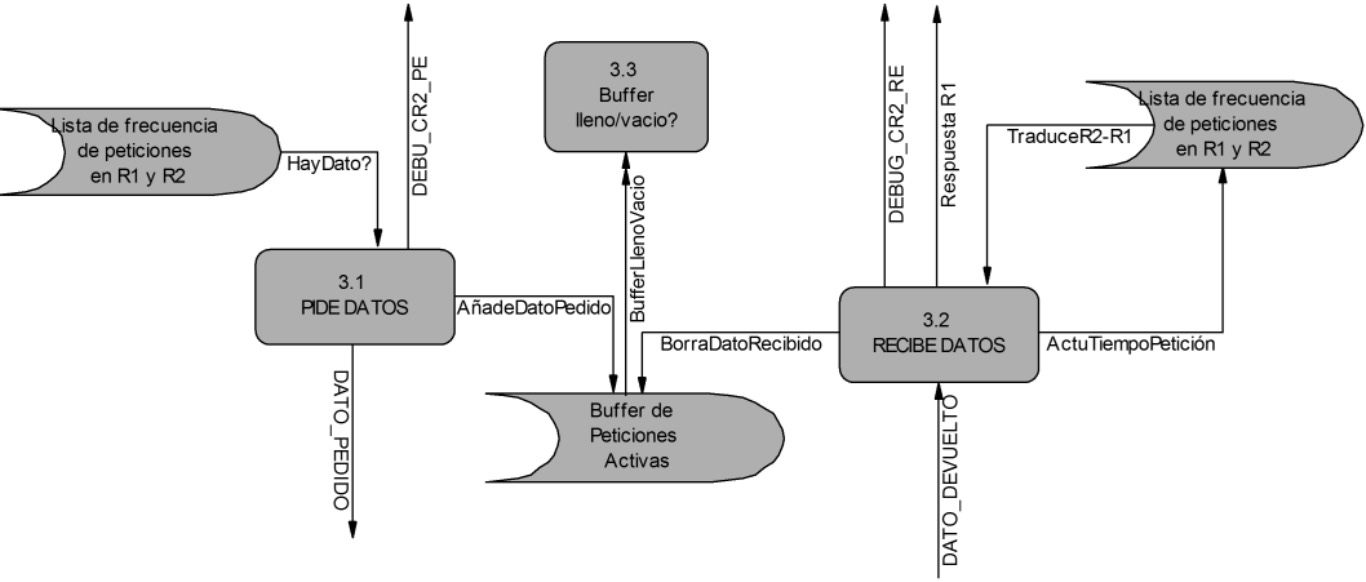
\includegraphics[width=0.8\linewidth]{Resources/diagramaA}
\end{figure}

\begin{figure}[H]
  \centering
  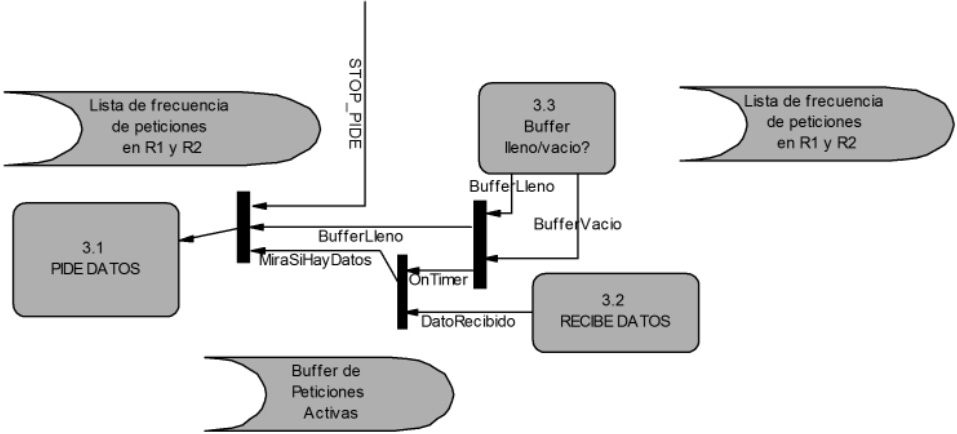
\includegraphics[width=0.8\linewidth]{Resources/diagramaB}
\end{figure}

\textit{Tema 5 Apartado 2.3}




\subsection{Comenta el proceso de elaboración de un plan de prueba seguido por el estándar IEEE 829 y los documentos asociados al proceso ¿Cuál es el estándar de ejecución de las pruebas? ¿Qué documentación implica?}
\textit{Tema 6 Apartado 3}

\subsubsection{Describe en qué consisten las pruebas funcionales, para qué sirven, en base a qué se construyen. Describe en detalle 3 técnicas de construcción de este tipo de pruebas.}
\textit{Tema 6 Apartado 4.1}


\newpage
\section{Caso práctico 2014}
Desarrollo del software asociado a un programador de control del sistema de climatización por aireación de una casa, que tiene, por lo menos, una pantalla táctil de 7 pulgadas para la interacción con el usuario.\\
El sistema de aireación puede mezclar aire frío tomado del exterior de la vivienda, con aire caliente, calentado por una caldera de Diesel.

\subsection{Detalla formalmente las siguientes funcionalidades, según el modelo empleado en las practicas}
\begin{itemize}
    \item RF1: Establecer una temperatura de confortt en modo manual
    \item RF2: Establecer la velocidad de ventilación del aire, de 0 a 5 posibilidades
    \item RF3: Establecer el modo de aireación (distribución posible del aire: la planta baja, al primer hangar, al segundo hangar, la toma de casa).
\end{itemize}
\textit{Comenzamos definimos el \textbf{actor usuario}, que será el único asociado a los requisitos funcionales aquí mencionados.\\
A partir de ahí creamos \textbf{un caso de uso para cada requisito funcional}.\\}


\subsubsection{Requisitos}
\begin{itemize}
\item \textbf{ID:} RF-0001
\item \textbf{Título:} Establecer una temperatura de confortt en modo manual.
\item \textbf{Descripción:} El sistema deberá permitir al usuario modificar la temperatura de una sala de manera manual a través de la pantalla táctil. Se permitirá un rango de temperaturas limitado. Se proporcionará frío o calor en función de la temperatura elegida por el usuario y la temperatura ambiente.
\item \textbf{Importancia:} Vital.
\item \textbf{Estabilidad:} Alta.
\item \textbf{Fuente:} Julián Flores González.
\item \textbf{Criterio de validación}: El sistema es capaz de regularse en función de la temperatura elegida por el usuario.
\end{itemize}
\begin{itemize}
\item \textbf{ID:} RF-0002
\item \textbf{Título:} Establecer velocidad de ventilación.
\item \textbf{Descripción:} El sistema deberá permitir al usuario modificar la velocidad de rotación de los ventiladores mediante el panel táctil. Se permiten las siguientes posibilidades:
\begin{itemize}
\item \textbf{0}: 0\% de rotación. 
\item \textbf{1}: 20\% de rotación. 
\item \textbf{2}: 40\% de rotación. 
\item \textbf{3}: 60\% de rotación. 
\item \textbf{4}: 80\% de rotación. 
\item \textbf{5}: 100\% de rotación. 
\end{itemize}
\item[] Donde el 100\% será la máxima capacidad de rotación y 0 significará que el ventilador está apagado.
\item \textbf{Importancia:} Vital.
\item \textbf{Estabilidad:} Alta.
\item \textbf{Fuente:} Julián Flores González.
\item \textbf{Criterio de validación}: el sistema es capaz de regular la velocidad de los ventiladores en función de lo que elija el usuario.
\end{itemize}

\begin{itemize}
\item \textbf{ID:} RF-0003
\item \textbf{Título:} Establecer modo de aireación.
\item \textbf{Descripción:} El sistema deberá permitir al usuario determinar que plantas de la casa se podrán ventilar con el sistema de climatización. Existen cuatro posibilidades únicamente:
\begin{itemize}
\item Planta baja: el sistema de climatización solo opera en la planta designada como 0.
\item Planta 1: el sistema de climatización solo opera en la planta designada como 1.
\item Planta 2: el sistema de climatización solo opera en la planta designada como 2.
\item Planta 3: el sistema de climatización solo opera en la planta designada como 3.
\end{itemize}
\item \textbf{Importancia:} Vital.
\item \textbf{Estabilidad:} Alta.
\item \textbf{Fuente:} Julián Flores González.
\item \textbf{Criterio de validación}: el sistema es capaz de climatizar las salas en función de lo elegido por el usuario.
\end{itemize}



\begin{enumerate}
    \item \textbf{Establecer temperatura de confortt}
    \begin{itemize}
        \item \textbf{Precondiciones:} El software debe tener un sistema climatización asociado.
    \item \textbf{PostCondiciones:} Se ha establecido la temperatura de confort indicada por el usuario para el sistema asociado.
    \item \textbf{Actores:} Usuario.
    \item \textbf{Descripción:}
    \begin{enumerate}[a.]
        \item El usuario selecciona el sistema de aire asociado sobre el que quiere realizar la acción.
        \item El sistema le muestra al usuario las acciones que puede realizar con el sistema de aire y el valor actual de sus parámetros, entre las acciones está la opción de modificar manualmente la temperatura de confort. El sistema no deja que este utilice rangos incorrectos.
        \item El usuario cambia la temperatura.
        \item El sistema en tiempo real modifica la temperatura de confort actual asociada a ese dispositivo.
    \end{enumerate}
    \end{itemize}

    \item \textbf{Establecer la velocidad de ventilación}
    \begin{itemize}
        \item \textbf{Precondiciones:} El software debe tener un sistema climatización asociado.
    \item \textbf{Postcondiciones:} Se ha establecido el modo de aireación indicado por el usuario.
    \item \textbf{Actores:} Usuario.
    \item \textbf{Descripción:}
    \begin{enumerate}[a.]
        \item El usuario selecciona el sistema de aire asociado sobre el que quiere realizar la acción.
        \item El sistema le muestra al usuario los parámetros. actuales y las acciones que puede realizar con el sistema de aire, entre ellas está la opción de modificar la velocidad de ventilación del aire entre los niveles 0 y 5.
        \item El usuario cambia el nivel de ventilación.
        \item El sistema en tiempo real modifica el nivel de ventilación actual asociada a ese dispositivo.
    \end{enumerate}
    \end{itemize}

    
    \item \textbf{Establecer el modo de aireación}
    \begin{itemize}
        \item \textbf{Precondiciones:} El software debe tener un sistema climatización asociado.
    \item \textbf{Postcondiciones:} Se ha establecido el modo de aireación indicada por el usuario para el sistema asociado.
    \item \textbf{Actores:} Usuario.
    \item \textbf{Descripción:}
    \begin{enumerate}[a.]
        \item El usuario selecciona el sistema de aire asociado sobre el que quiere realizar la acción.
        \item El sistema le muestra al usuario los parámetros actuales del sistema y la acciones que puede realizar sobre esos parámetros, entre estas acciones está la de establecer el modo de aireación entre los modos (planta baja, primer hangar, segundo hangar, toma de casa).
        \item El usuario cambia el modo de aireación.
        \item El sistema en tiempo real modifica el modo de aireación asociada a ese dispositivo.
    \end{enumerate}
    \end{itemize}

    
\end{enumerate}

\subsection{Diseña el Modelo de Contexto y el DFD de primer nivel de forma que englobe las funcionalidades del apartado anterior.}

%TODO añadir foto
\begin{figure}[H]
  \centering
  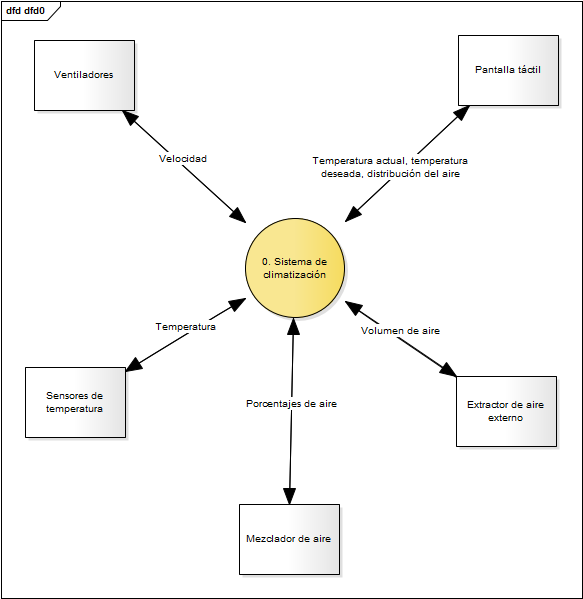
\includegraphics[width=0.8\linewidth]{Resources/dfd0.png}
  \caption{Diagrama de contexto}
  \label{fig:dfd0}
\end{figure}
\begin{figure}[H]
  \centering
  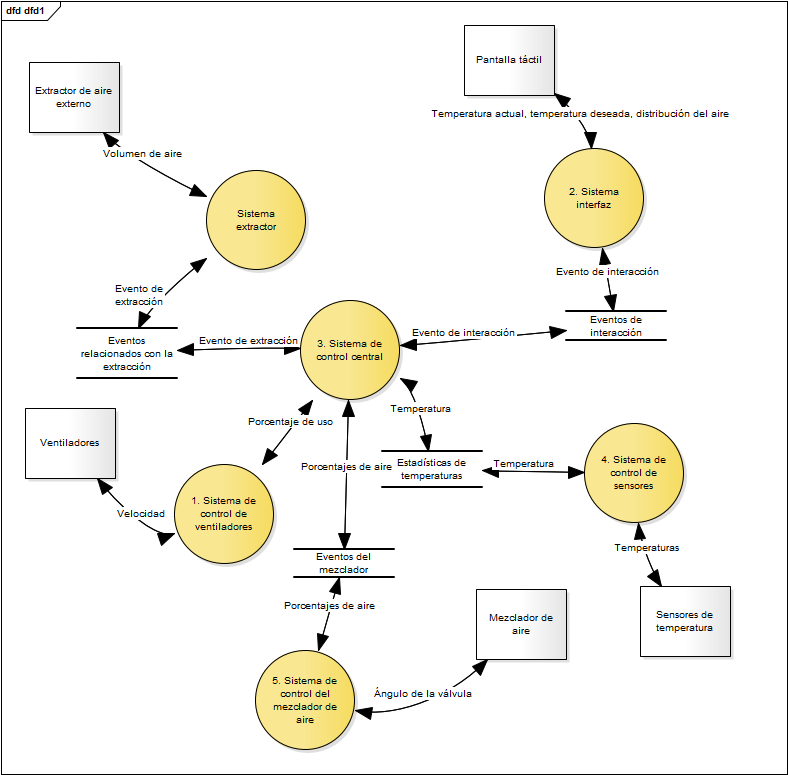
\includegraphics[width=0.8\linewidth]{Resources/dfd1.png}
  \caption{DFD de primer nivel}
  \label{fig:dfd1}
\end{figure}

\subsection{Para la funcionalidad RF1, haz un DFD de nivel 2, con su DFC asociado}


\subsection{En el siguiente contexto ¿cual sería el modelo de ciclo de vida más adecuado? justifica tu respuesta.}
``El software va a ser desarrollado por un empresa de amplia experiencia en el desarrollo de software empotrado, pero nunca para el sector de vivienda familiar. Los requisitos están perfectamente definidos, pero la competencia está muy activa, lo que puede resultar en una modificación de requisitos para adoptarlo a las nuevas funcionalidades. Las pantallas táctiles están empezando a ser comercializadas por lo que no se sabe muy bien como es el paradigma de iteración con el usuario''
%XP o Espiral??

\paragraph{Una posible solución:} El ciclo de vida recomendado es el ``ciclo de vida en espiral''. Los motivos son los siguientes:
\begin{itemize}
\item Los requisitos están bien definidos y los únicos cambios posibles parecen ser la adaptación de nuevas funcionalidades. Como se suceden en varias iteraciones es trivial incorporar esto.
\item No se sabe como es el paradigma de interacción con el usuario por lo que interesa crear prototipos para ello. Este ciclo de vida lo permite (pues en cada iteración hay que tener un producto ejecutable). Además, hay que tener en cuenta que la inexperiencia en el sector familiar refuerza este argumento pues varias iteraciones permiten refinar y mejorar el producto.
\end{itemize}

\subsection{Establece el proceso de admisión de riesgos, según la metodología de Sommerville, que contempla solo 2 riesgos, para el desarrollo de software en el siguiente contexto}
``Vamos a adquirir pantallas táctiles a una empresa china que opera por internet. Tenemos un simulador para el desarrollo de software, que emula el entorno de la vivienda pero no es muy estable, y además no tenemos acceso continuado al prototipo de vivienda en la que se va a verificar y validar el software.

\begin{enumerate}
    \item \textbf{Retraso en la realización de pruebas}
    
    \begin{itemize}
    \item \textbf{Descripción:} Problemas de estabilidad en el software de pruebas o incapacidad para probar el software en un entorno real pueden producir retrasos tanto en el desarrollo normal como en la realización de las pruebas del software.
    \item \textbf{Probabilidad:} Alto.
    \item \textbf{Impacto:} Serio.
    \item \textbf{Tipo de riesgo:} Del Proyecto.
    \item \textbf{Tratamiento:} Minimización.
    \item \textbf{Acción:} Toma de contacto por parte de nuestro equipo con el simulador utilizado antes de las pruebas en si del programa, para conocer que errores da este y no confundirlos con errores del software desarrollado.
    \item \textbf{Secuencia de seguimiento:} Semanal.
    \item \textbf{Indicadores de riesgo:} 
    \begin{itemize}
        \item La realización de pruebas se retrasa durante la fase de utilización de la simulación en las pruebas.
        \item imposibilidad de encontrar un lugar donde hacer la verificación y validación definitivas.
        \item Surgen reportes de fallos del software de simulación durante las pruebas que deberían haberse detectado durante la toma de contacto de nuestro equipo con el software de simulación.
    \end{itemize}
    \end{itemize}

    \item \textbf{Corrupción de todos los archivos del proyecto}
    \begin{itemize}
    \item \textbf{Descripción:} el simulador, debido a su baja estabilidad, corrompe todos los archivos del proyecto.
    \item \textbf{Probabilidad antigua:} Medio.
    \item \textbf{Probabilidad nueva:} Medio.
    \item \textbf{Impacto antiguo:} Catastrófico.
    \item \textbf{Impacto nuevo:} Tolerable.
    \item \textbf{Tipo de riesgo:} Del Producto.
    \item \textbf{Tratamiento:} Minimización.
    \item \textbf{Acción:} Se establecerá un proceso de gestión de la configuración que almacenará en un control de versiones copias diarias de los archivos a utilizar por el simulador.
    \item \textbf{Secuencia de seguimiento:} Diaria.
    \item \textbf{Indicadores de riesgo:}
    \begin{itemize}
        \item Incapacidad de acceder a los archivos del proyecto.
    \end{itemize}
    \end{itemize}
\end{enumerate}


\subsection{Pensando en un proceso de pruebas, establece las clases de equivalencia para las siguientes entradas, asumiendo que en la pantalla táctil se puedan introducir los datos por pantalla con la simulación de un teclado qwerty}
%no entiendo si quiere que todos los datos sean tipo string o algo....
\begin{enumerate}
    \item Temperatura de confort.
    \item Velocidad del ventilador.
    \item Válvula que regula la mezcla aire frío/caliente, asumiendo que la regulación de la misma es por porcentaje, desde 0 (solo aire frío) hasta 100 (solo aire caliente). Cualquier otro valor en el intervalo [0--100] dará una mezcla\%aire\_caliente+\%aire\_frío, de forma que \%aire\_frío=``valor'' y \%aire\_frío=100-``valor''. Este valor no es establecido por teclado, es una variable interna de nuestro software.
\end{enumerate}

%Decimos que es un entero y no un float para no complicar la marrana con los .
\begin{table}[H]
\centering

\resizebox{\textwidth}{!}{%
\begin{tabular}{|c|c|c|c|c|c|c|}
\hline
\multirow{2}{*}{Información} & \multirow{2}{*}{Tipo dato} & \multirow{2}{*}{Regla} & \multicolumn{2}{c|}{Clase válida} & \multicolumn{2}{c|}{Clase no válida} \\ \cline{4-7} 
                             &                            &                        & Id   & Dominio                    & Id         & Dominio                 \\ \hline
Temperatura\_confort         & Entero positivo & 1                      & 1    & {[}10, 45{]}               & 2          & {[}0, 10)               \\ \hline
                             &                            &                        &      &                            & 3          & (45, +inf)              \\ \hline
                             &                            & 3                      & 4    & Está compuesto de dígitos  & 5          & Contiene letras         \\ \hline
\end{tabular}
}
\caption{Clases de equivalencia para ``Temperatura confort''}
\end{table}

%Es la regla 2o la cuatro?
\begin{table}[H]
\centering
\resizebox{\textwidth}{!}{%
\begin{tabular}{|c|c|c|c|c|c|c|}
\hline
\multirow{2}{*}{Información} & \multirow{2}{*}{Tipo dato} & \multirow{2}{*}{Regla} & \multicolumn{2}{c|}{Clase válida} & \multicolumn{2}{c|}{Clase no válida} \\ \cline{4-7} 
                             &                            &                        & Id          & Dominio             & Id           & Dominio               \\ \hline
Velocidad\_ventilador        & Entero positivo            & 2                      & 1           & {[}0, 5{]}          & 2            & (-inf, -1{]}          \\ \hline
                             &                            &                        & 8           & 2                   & 3            & {[}6, +inf)           \\ \hline
                             &                            &                        & 4           & 3                   &              &                       \\ \hline
                             &                            &                        & 5           & 4                   &              &                       \\ \hline
                             &                            &                        & 6           & 5                   &              &                       \\ \hline
                             &                            &                        & 7           & 0                   &              &                       \\ \hline
\end{tabular}
}
\caption{Clases de equivalencia para ``Velocidad del ventilador''}
\end{table}

% Lo hago solo para el valor, que es lo que hay que probar
\begin{table}[h]
\centering
\resizebox{\textwidth}{!}{%
\begin{tabular}{|c|c|c|c|c|c|c|}
\hline
\multirow{2}{*}{Información} & \multirow{2}{*}{Tipo dato} & \multirow{2}{*}{Regla} & \multicolumn{2}{c|}{Clase válida} & \multicolumn{2}{c|}{Clase no válida} \\ \cline{4-7} 
                             &                            &                        & Id         & Dominio              & Id           & Dominio               \\ \hline
Valor\_mezcla                & Punto flotante             & 1                      & 1          & {[}0, 100{]}         & 2            & (-inf, 0)             \\ \hline
                             &                            &                        &            &                      & 3            & (100, +inf)           \\ \hline
\end{tabular}
}
\caption{Clases de equivalencia para el ``valor de la mezcla''}
\end{table}

% \begin{figure}[H]
%   \centering
%   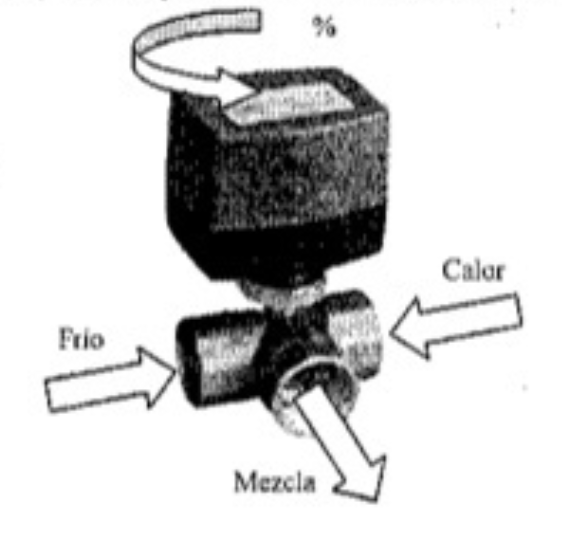
\includegraphics[width=0.5\linewidth]{Resources/imagenExamen2014}
%   \caption{Funcionamiento del aire}
%   \label{fig:aireAcondicionado}
% \end{figure}

\newpage
\section{Caso práctico 2014}

Desarrollo del software asociado a un cajero automático de un banco genérico, llamémosle \textbf{RABENSO}.

\subsection{Detalla formalmente las siguientes funcionalidades, según el modelo empleado y la plantilla que empleasteis en las prácticas}
\begin{itemize}
    \item RF1: Cambiar PIN.
    \item RF2: Consultar movimientos anteriores.
    \item RF3: Retirar dinero.
\end{itemize}

\begin{itemize}
\item \textbf{ID:} RF-0001
\item \textbf{Título:} Cambiar pin.
\item \textbf{Descripción:} el sistema deberá permitir cambiar el número de identificación personal del usuario utilizado para autorizar transacciones bancarias. Para ello utilizará una interfaz gráfica con un teclado numérico virtual en pantalla y confirmación de pin anterior. Si el número anterior no es correcto no se realizará ningún cambio de PIN.
\item \textbf{Importancia:} Vital.
\item \textbf{Estabilidad:} Alta.
\item \textbf{Fuente:} Julián Flores González.
\item \textbf{Criterio de validación}: el sistema cambia el número de identificación según las directrices anteriormente especificadas.
\end{itemize}

\begin{itemize}
\item \textbf{ID:} RF-0002
\item \textbf{Título:} Consultar movimientos.
\item \textbf{Descripción:} el sistema deberá mostrar todos los movimientos del usuario en una lista desplegable por pantalla. Deberá permitir filtrar los movimientos por fecha (es decir, especificar un rango de fechas para visualizar).
\item \textbf{Importancia:} Vital.
\item \textbf{Estabilidad:} Alta.
\item \textbf{Fuente:} Julián Flores González.
\item \textbf{Criterio de validación}: El sistema muestra el conjunto de movimientos correctamente.
\end{itemize}

\begin{itemize}
\item \textbf{ID:} RF-0003
\item \textbf{Título:} Retirar dinero.
\item \textbf{Descripción:} el sistema deberá retirar dinero de la cuenta bancaria del usuario. Para ello, se sustrae la cantidad especificada por el usuario en el teclado numérico virtual habilitado para tal propósito y se dispone un conjunto de billetes con dicha cantidad (minimizando el número de billetes emitidos).
\item \textbf{Importancia:} Vital.
\item \textbf{Estabilidad:} Alta.
\item \textbf{Fuente:} Julián Flores González.
\item \textbf{Criterio de validación}: el sistema realiza las operaciones correctamente (sustracción y emisión de billetes).
\end{itemize}

\subsection{Diseña el modelo de contexto, el DFD de primer nivel de forma que solo englobe las funcionalidades del apartado anterior}

\subsection{Para el RF3, haz el DFD de nivel 2, con su correspondiente DFC asociado}

\subsection{En el siguiente contexto, ¿cuál sería el modelo de ciclo de vida más apropiado? Motiva tu respuesta:}
``El software va a ser desarrollado por una empresa que amplia experiencia en el desarrollo software bancario. Los requisitos están perfectamente definidos, pero el cliente quiere dotar al cajero de funcionalidades adicionales a las clásicas que le darían una ventaja competitiva sobre la competencia (que es muy activa), lo que exige resultados operativos a corto plazo.''
%También podría ser espiral por lo mismo que en 2014
El ciclo de vida elegido es ``Programación Extrema'' por los siguientes motivos:
\begin{itemize}
    \item La dinámica de historias de usuario permite al cliente priorizar las funcionalidades que quiera por lo que es útil si se requieren resultados a corto plazo.
    \item La dinámica de historias de usuario proporciona entregables frecuentes lo que posibilita tener resultados operativos a corto plazo.
    \item Al ser una metodología ágil, tiene una menor carga de modelos y documentación en comparación con las metodologías clásicas por lo que las entregas serán más rápidas.
\end{itemize}

\subsection{Establece un proceso de administración de riesgos, siguiendo la metodología de Sommerville, que contemple solo 3 riesgos, para el desarrollo del software en el siguiente contexto:}
``El cajero tiene que admitir tarjetas de los siguientes tipos: RB, Rabocard, ENSO, TaboaBank. Tiene que tener un funcionamiento 24/7. Sabemos que en el mercado hay competidores que están trabajando en un producto similar''

\subsubsection{Identificación y análisis de riesgos}
%Aquí lo voy a realizar por separado
\begin{itemize}
\item \textbf{ID}: R-001
\item \textbf{Nombre}: Aparece un nuevo tipo de tarjeta de crédito.
\item \textbf{Descripción}:
\end{itemize}

\begin{itemize}
    \item \textbf{ID}: R-002
    \item \textbf{Nombre}: el cajero deja de dar servicio debido a un error de software.
    \item \textbf{Descripción}: Un error de software provoca que el cajero quede inutilizado. 
\end{itemize}

\begin{itemize}
    \item \textbf{ID}: R-003
    \item \textbf{Nombre}: Un competidor crea un producto similar que supera en funcionalidades nuestro producto.
\end{itemize}

\subsubsection{Planificación de riesgos}


\subsection{Pensando en el proceso de pruebas, establece las clases de equivalencia para las siguientes entradas:}
\begin{itemize}
    \item Tipo de tarjeta
    \item PIN
    \item ¿Desea imprimir el recibo?
\end{itemize}
\newpage
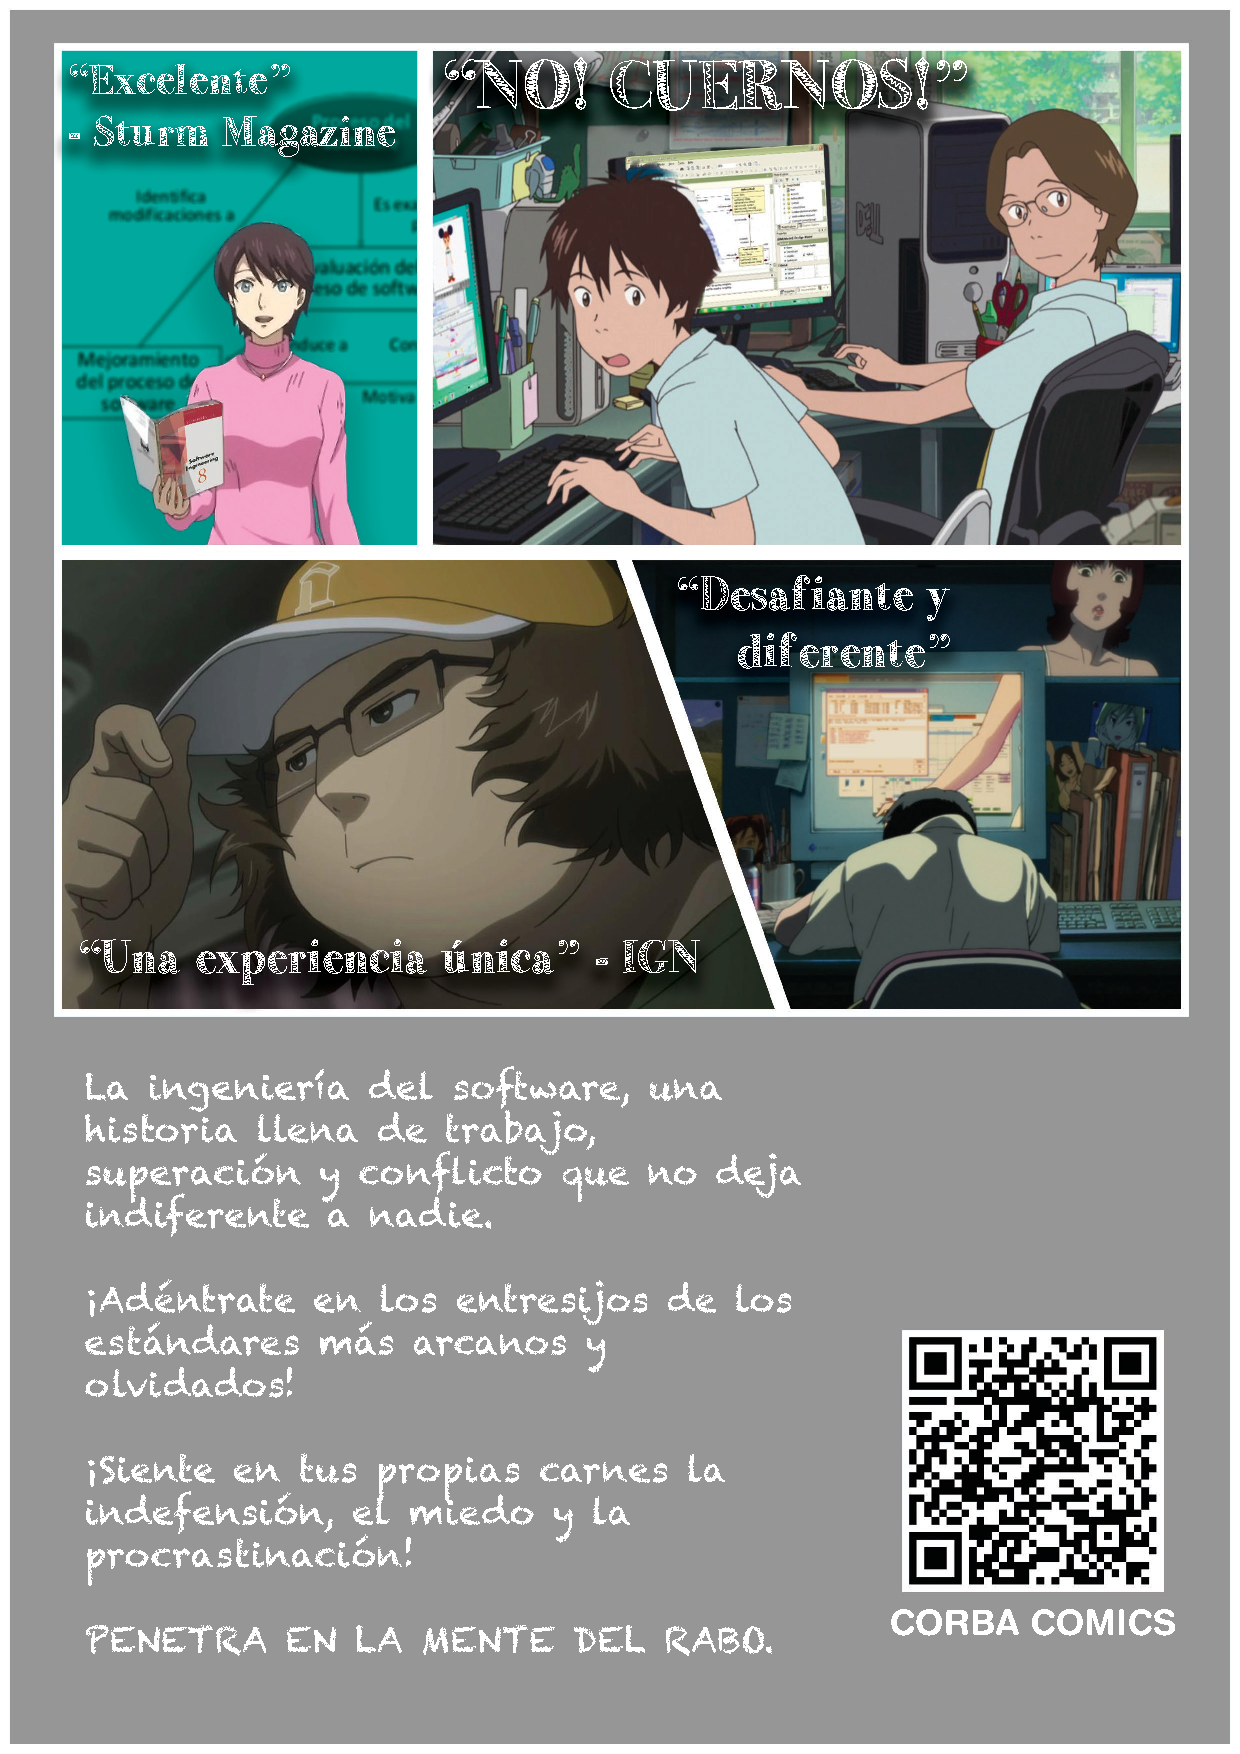
\includepdf{Resources/CONTRAPORTADA}
\end{document}
